\section{Neutron Multiplicities \& Energy}
\label{app:Neutron_Multiplicities}

This appendix includes all the plots not shown in Section~\ref{subsec:N_multiplicities_Energy}. 
For full description of the files, please make reference to that section.
The plots will be put in the same order as before. 

\subsection{$\nu$ Plots}

\subsubsection{CCQE}

\begin{figure}[!htb]
\centering
\begin{subfigure}[b]{0.32\textwidth}
  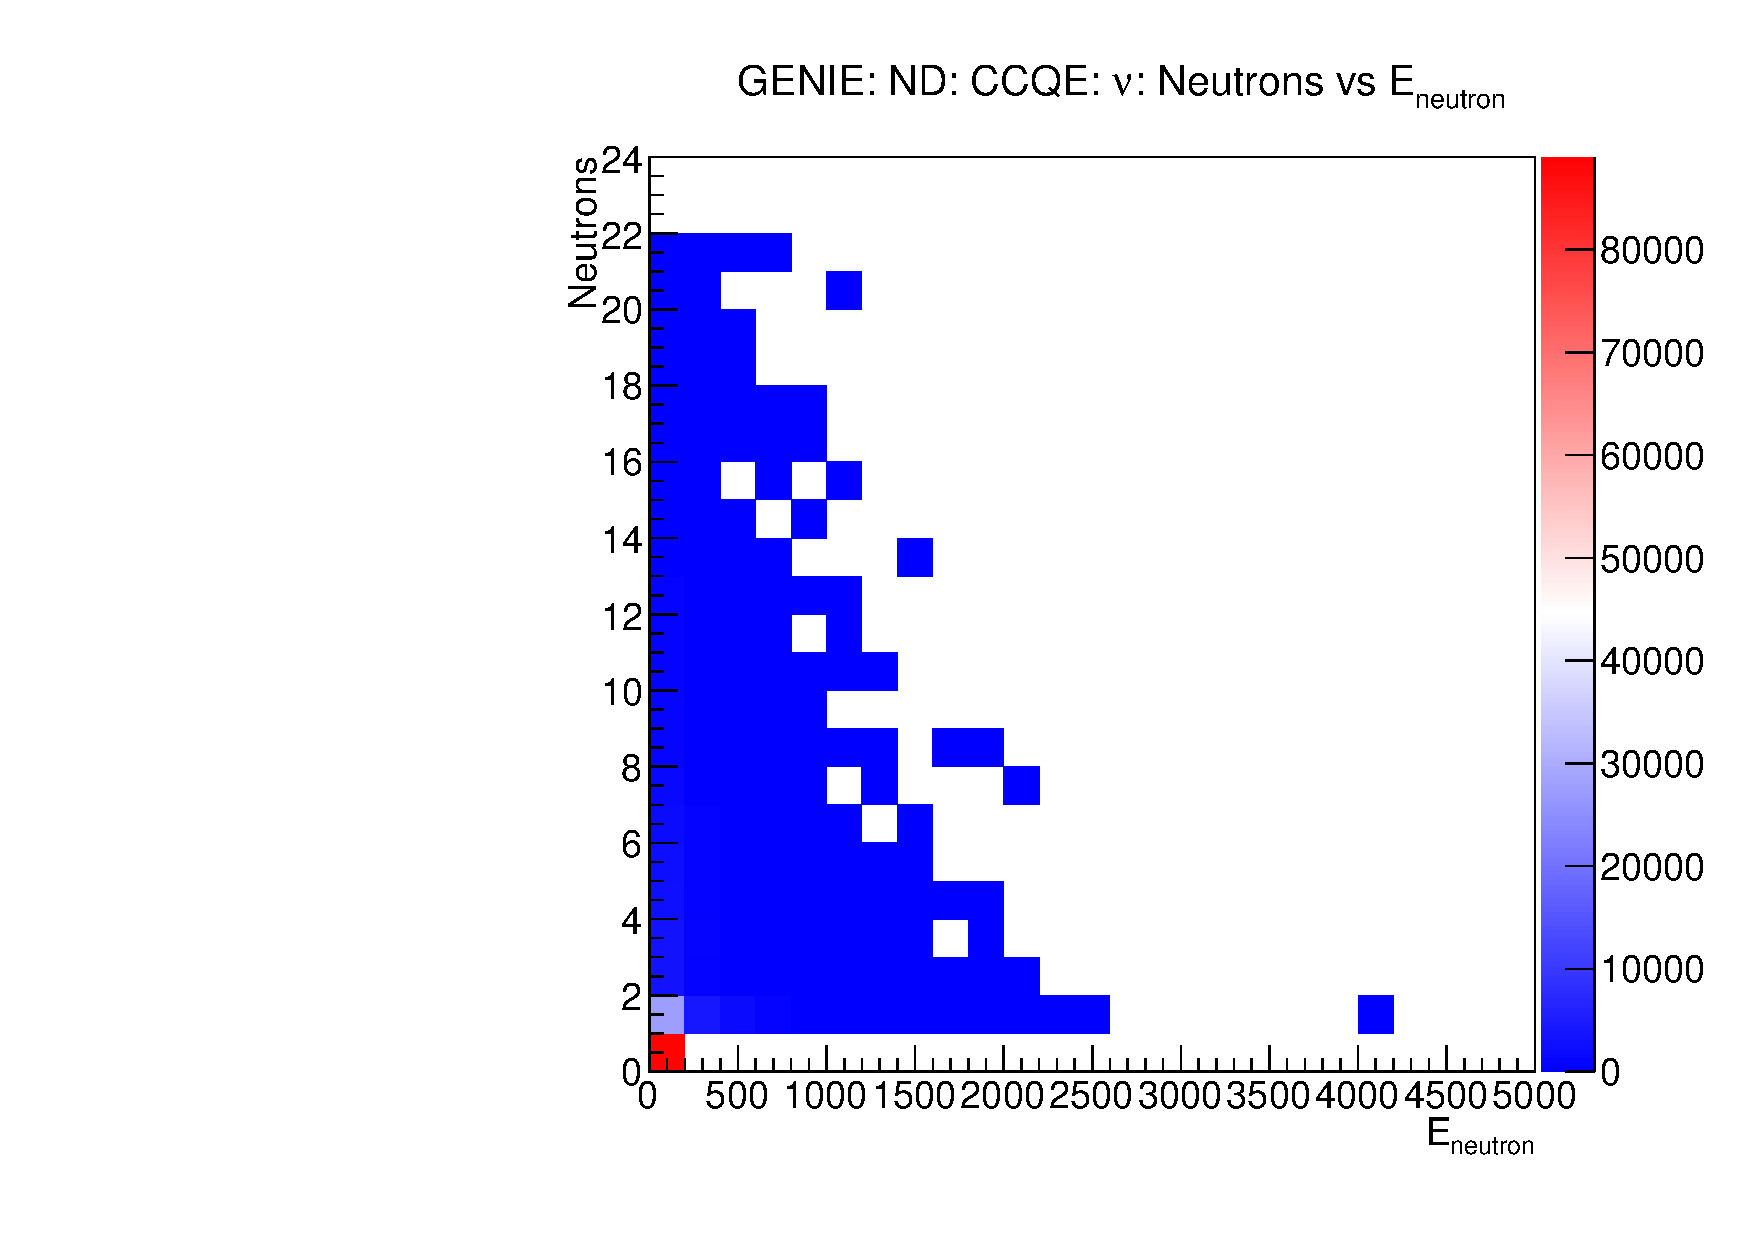
\includegraphics[width=\textwidth]{nneutrons_v_total_ene/Nneutrons_Total_ENe_ccqe_GENIE_ND_numu.pdf}
\end{subfigure}
\begin{subfigure}[b]{0.32\textwidth}
  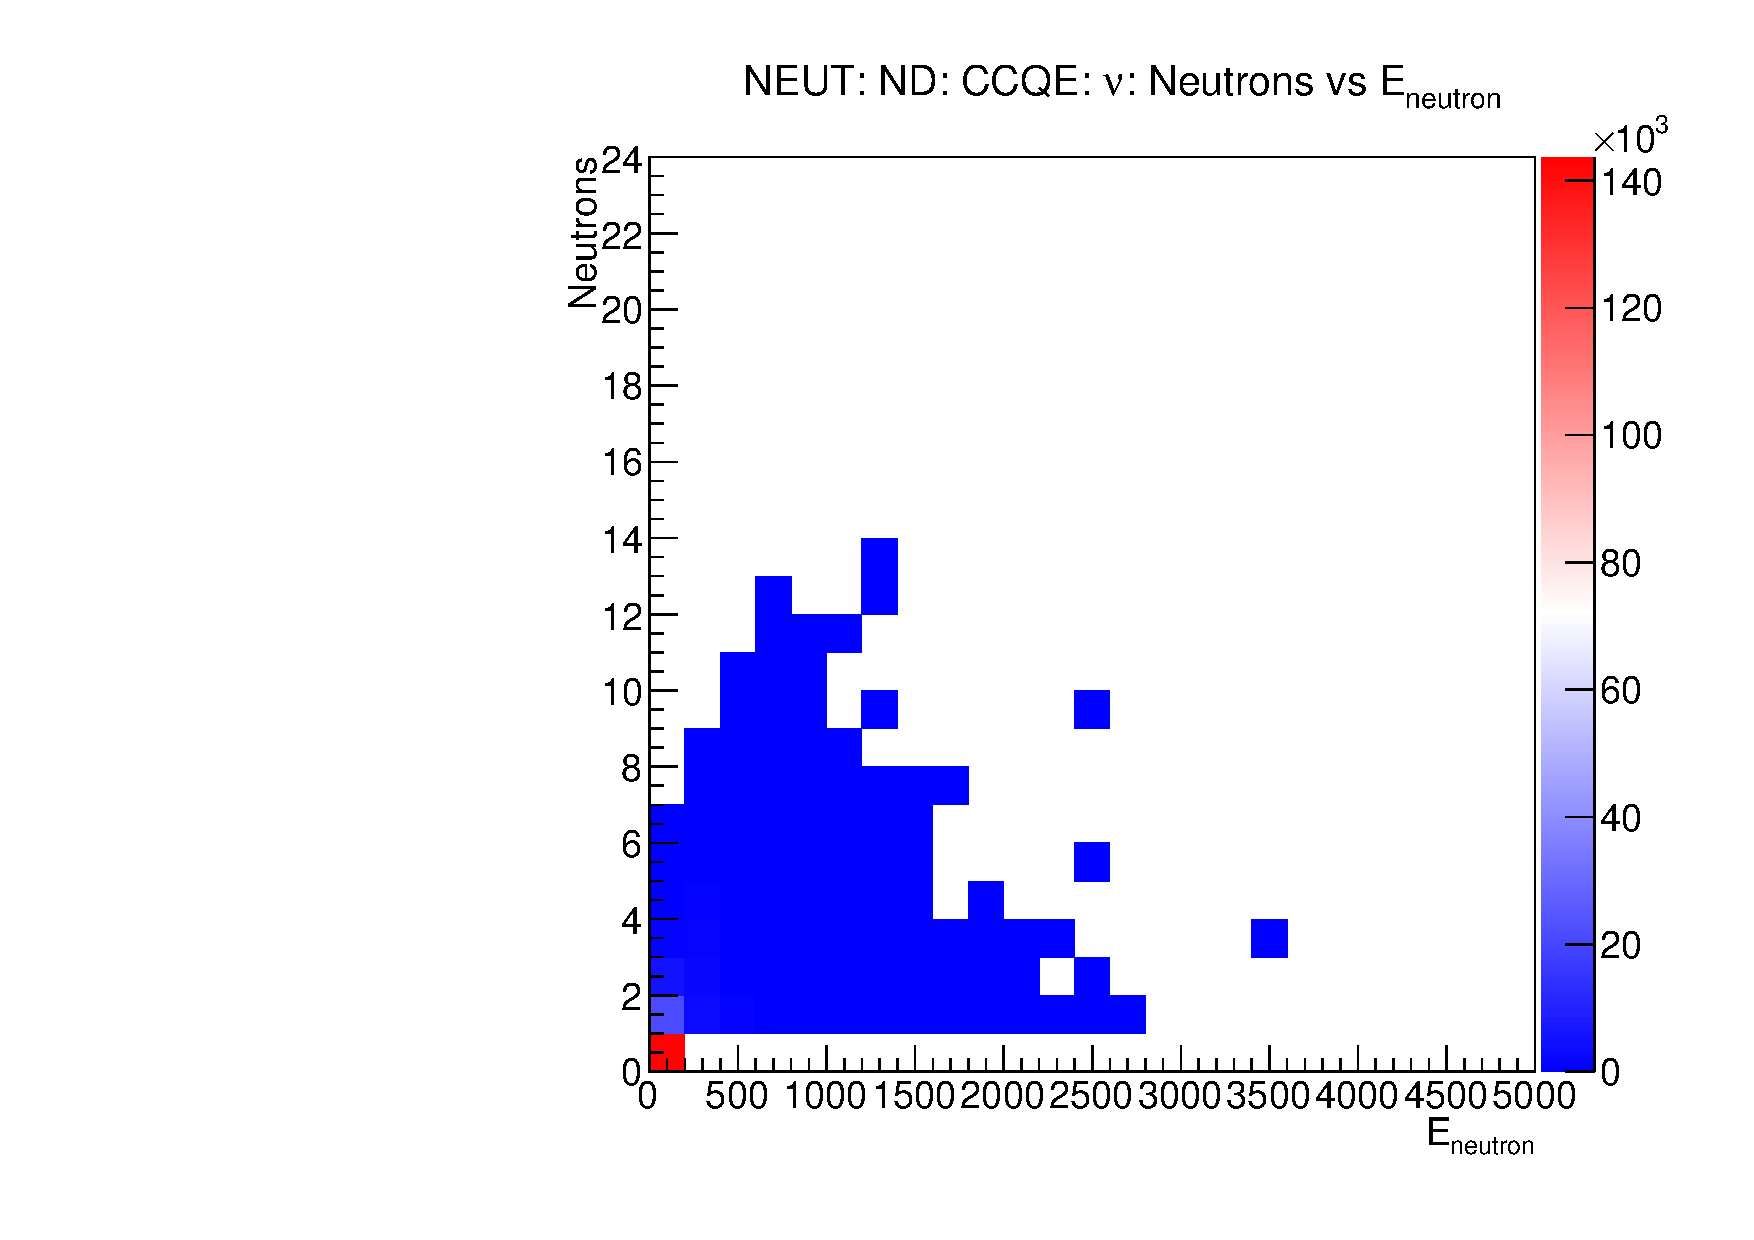
\includegraphics[width=\textwidth]{nneutrons_v_total_ene/Nneutrons_Total_ENe_ccqe_NEUT_ND_numu.pdf}
\end{subfigure}
\begin{subfigure}[b]{0.32\textwidth}
  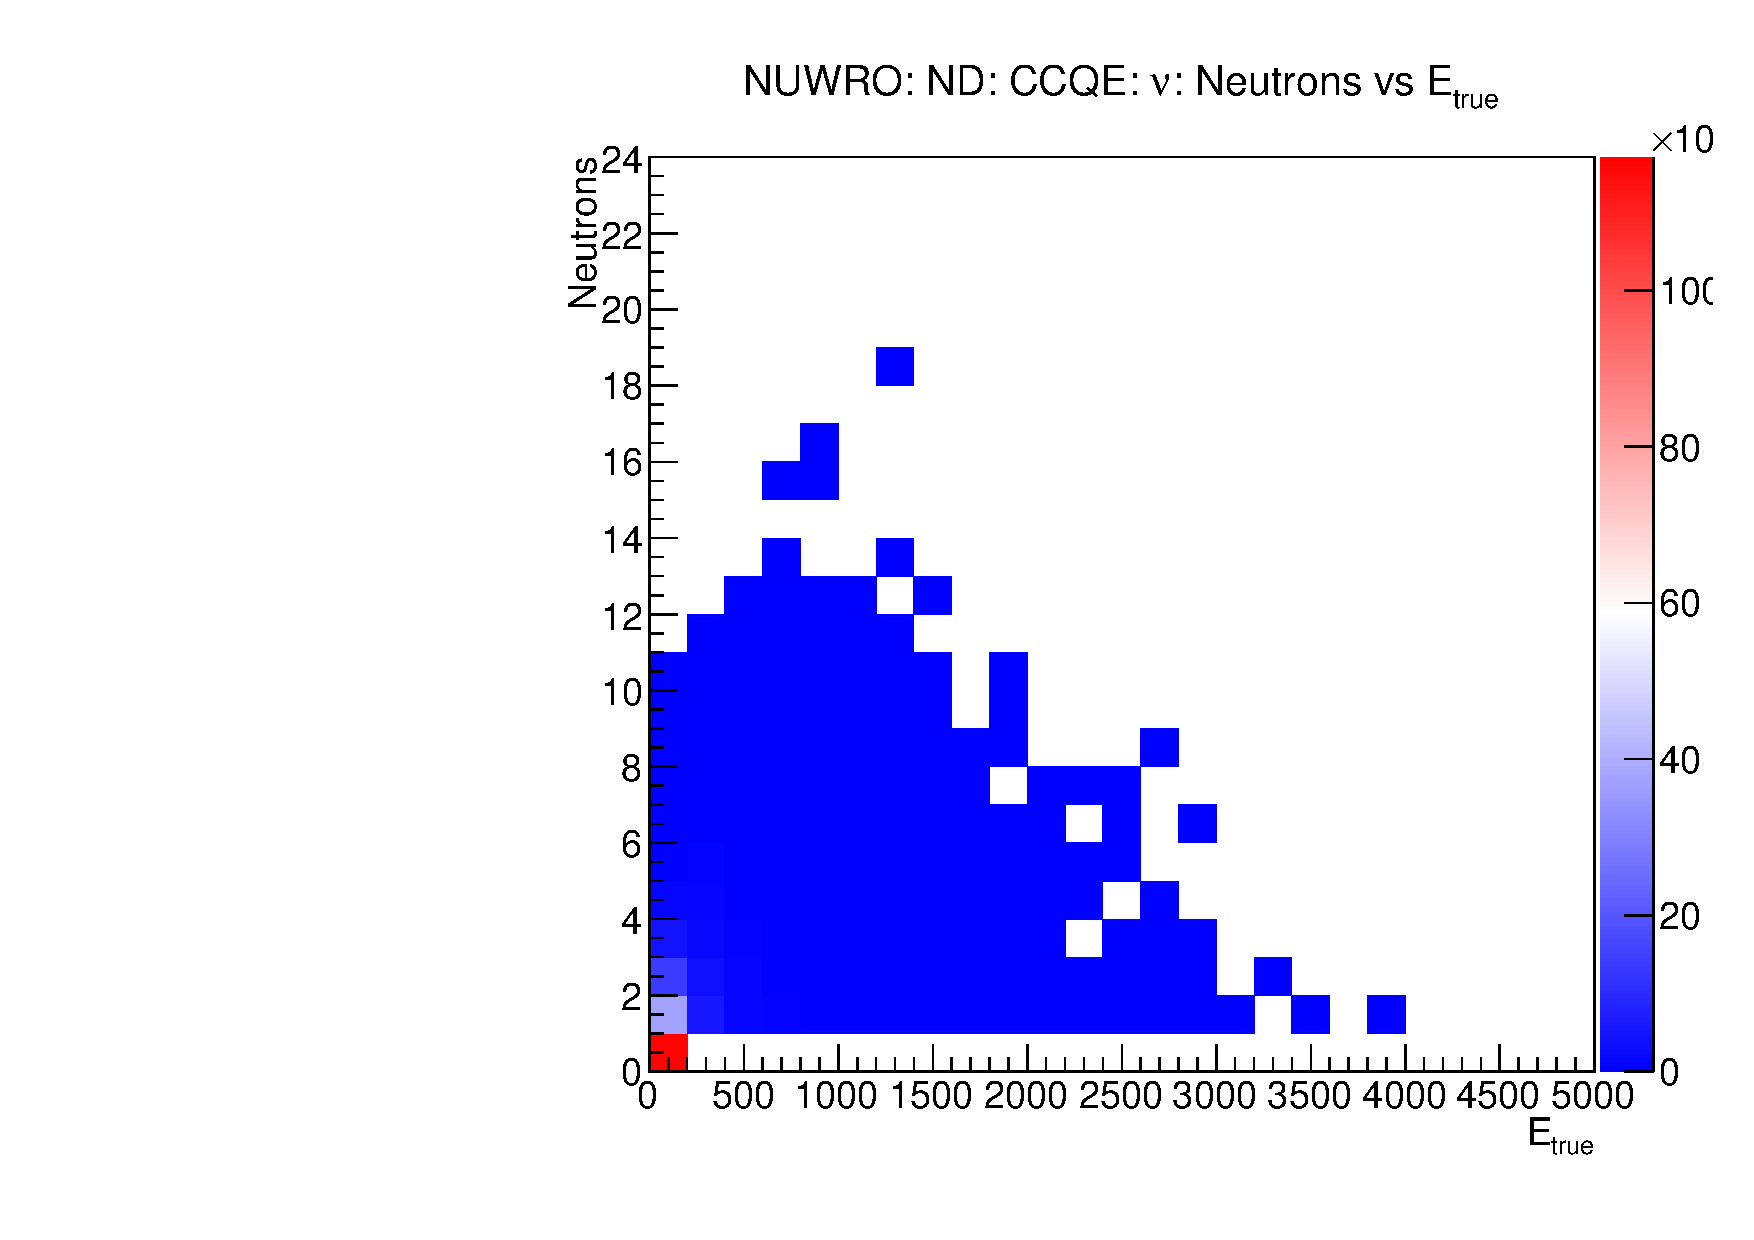
\includegraphics[width=\textwidth]{nneutrons_v_total_ene/Nneutrons_Total_ENe_ccqe_NUWRO_ND_numu.pdf}
\end{subfigure}
\end{figure}

\begin{figure}[!htb]
\centering
\begin{subfigure}[b]{0.32\textwidth}
  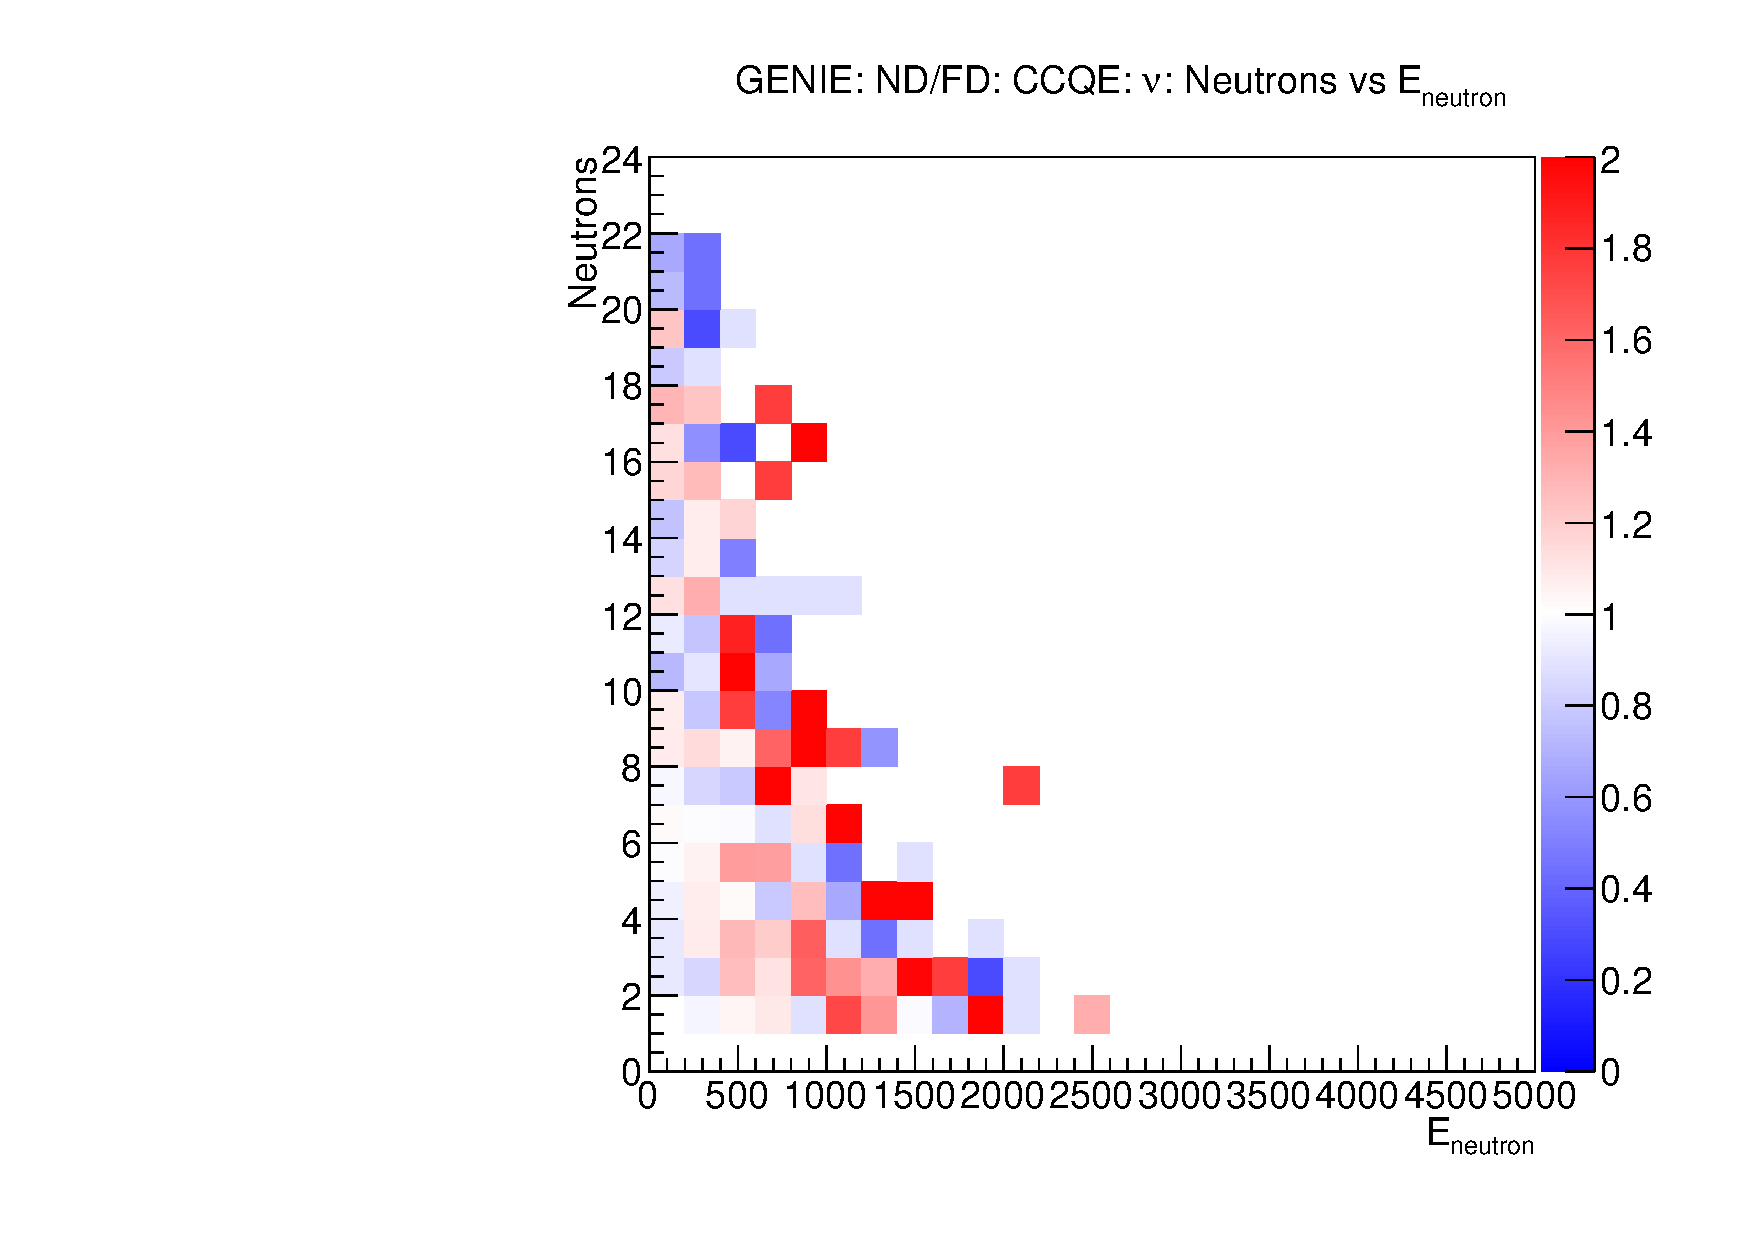
\includegraphics[width=\textwidth]{nneutrons_v_total_ene/Nneutrons_Total_ENe_ccqe_GENIE_ND_FD_numu_norm.pdf}
\end{subfigure}
\begin{subfigure}[b]{0.32\textwidth}
  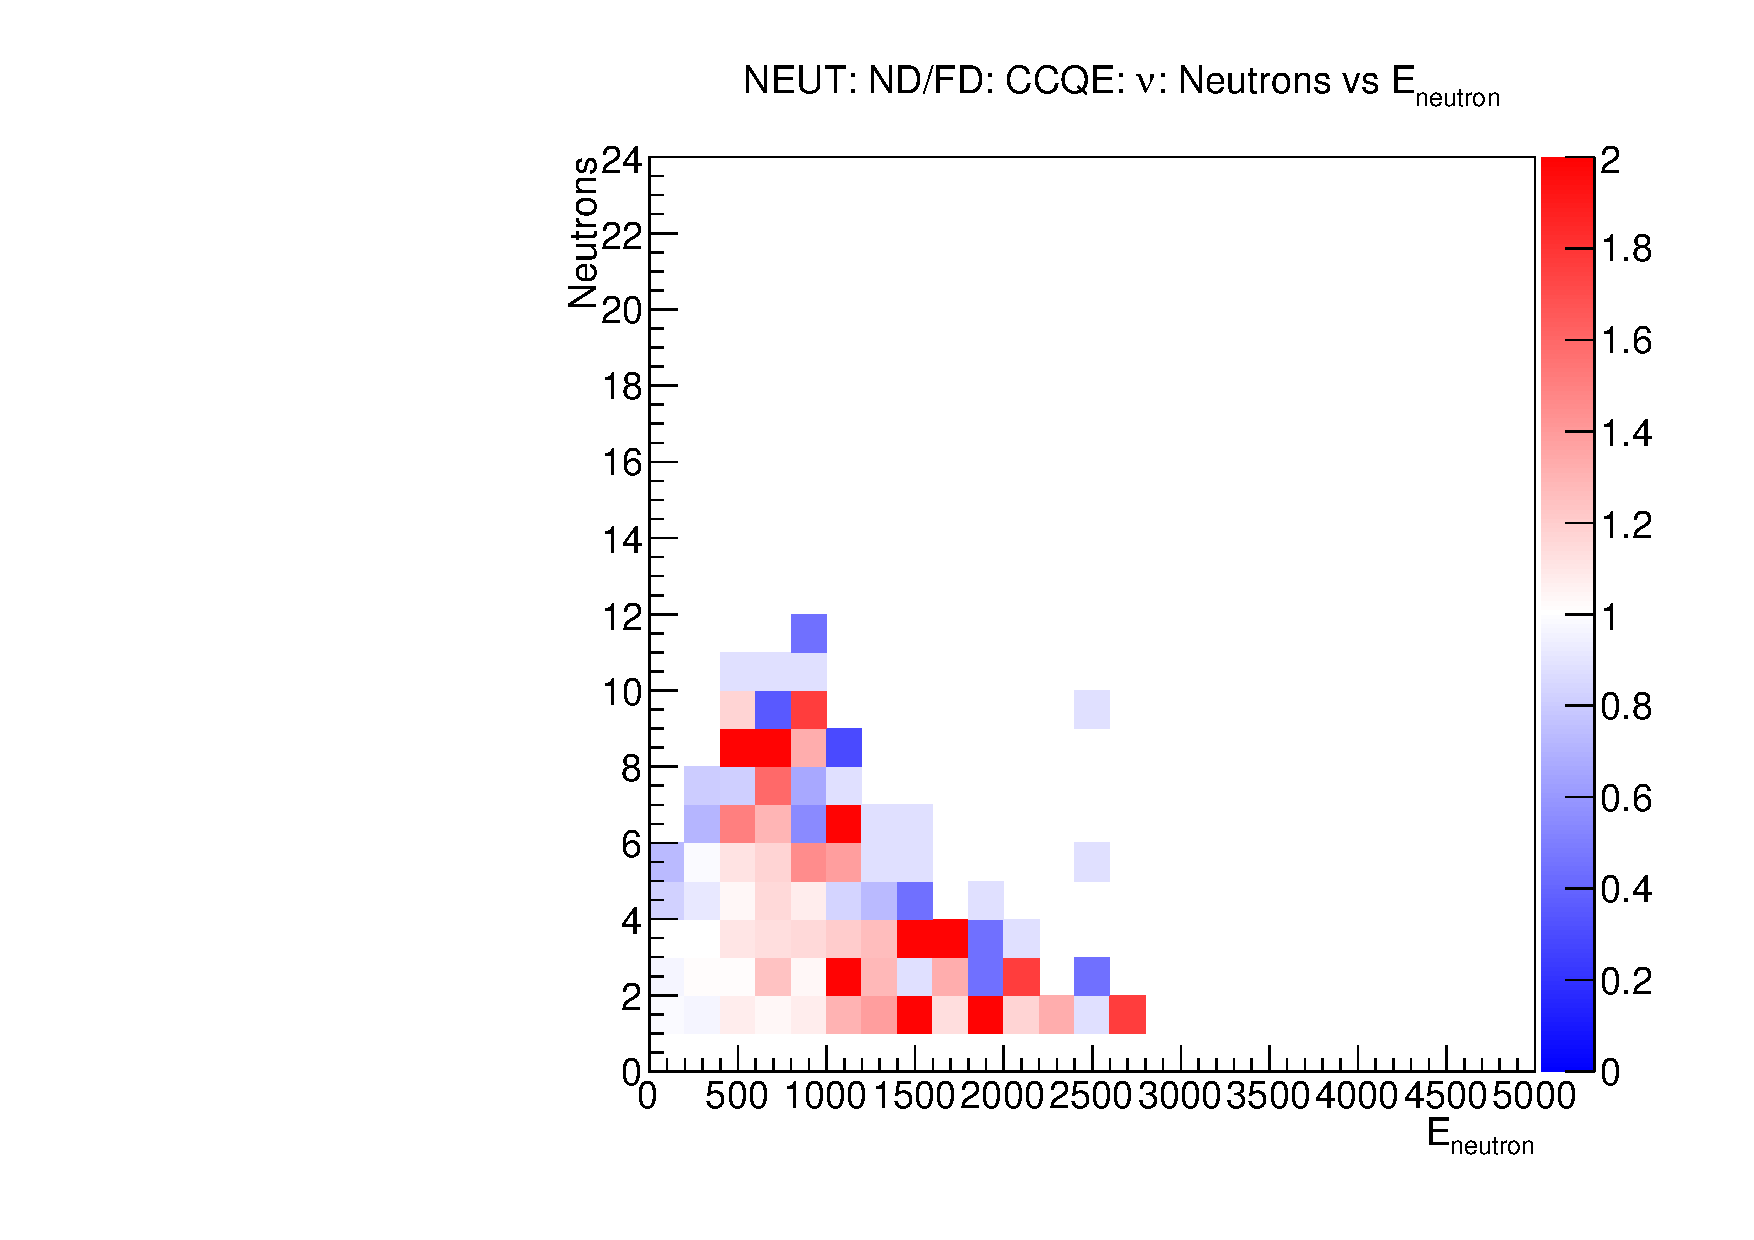
\includegraphics[width=\textwidth]{nneutrons_v_total_ene/Nneutrons_Total_ENe_ccqe_NEUT_ND_FD_numu_norm.pdf}
\end{subfigure}
\begin{subfigure}[b]{0.32\textwidth}
  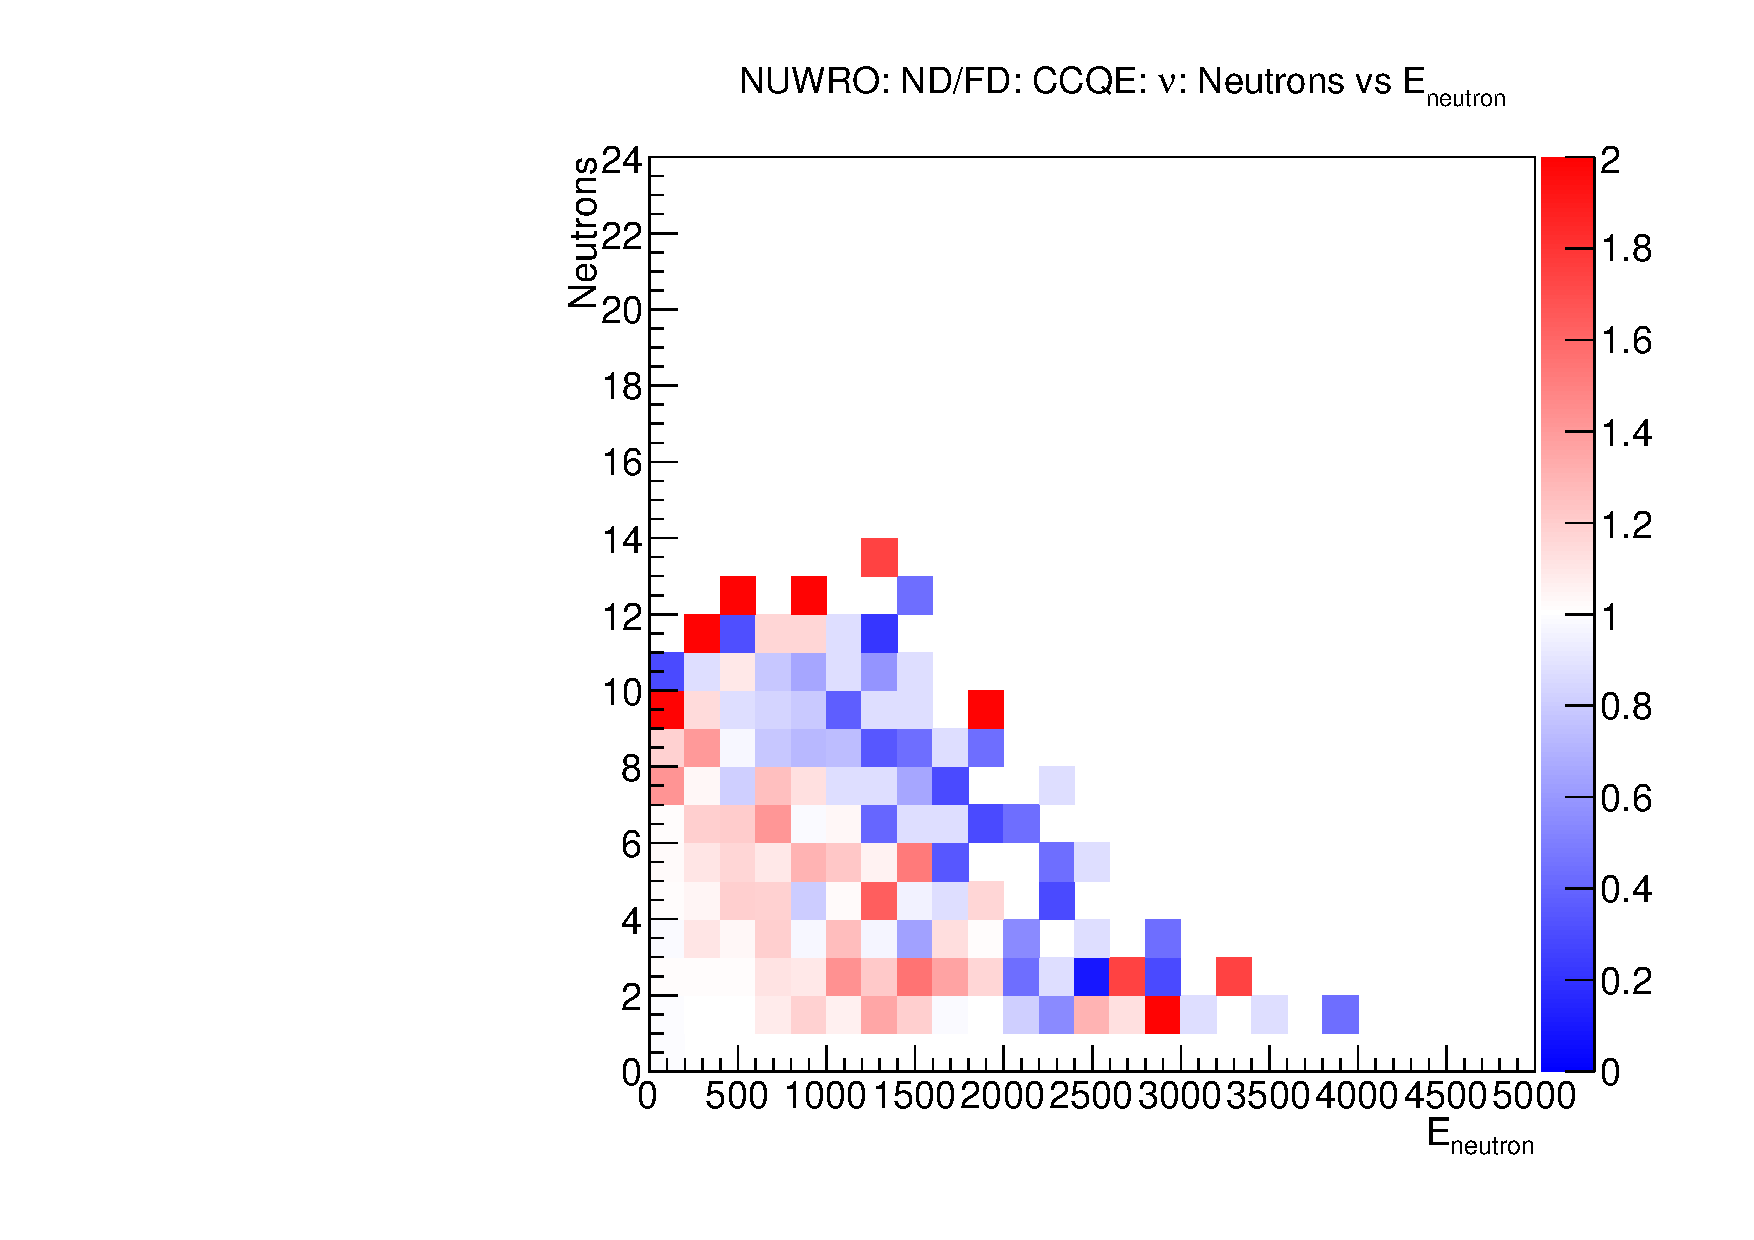
\includegraphics[width=\textwidth]{nneutrons_v_total_ene/Nneutrons_Total_ENe_ccqe_NUWRO_ND_FD_numu_norm.pdf}
\end{subfigure}
\end{figure}

\begin{figure}[!htb]
\centering
\begin{subfigure}[b]{0.32\textwidth}
  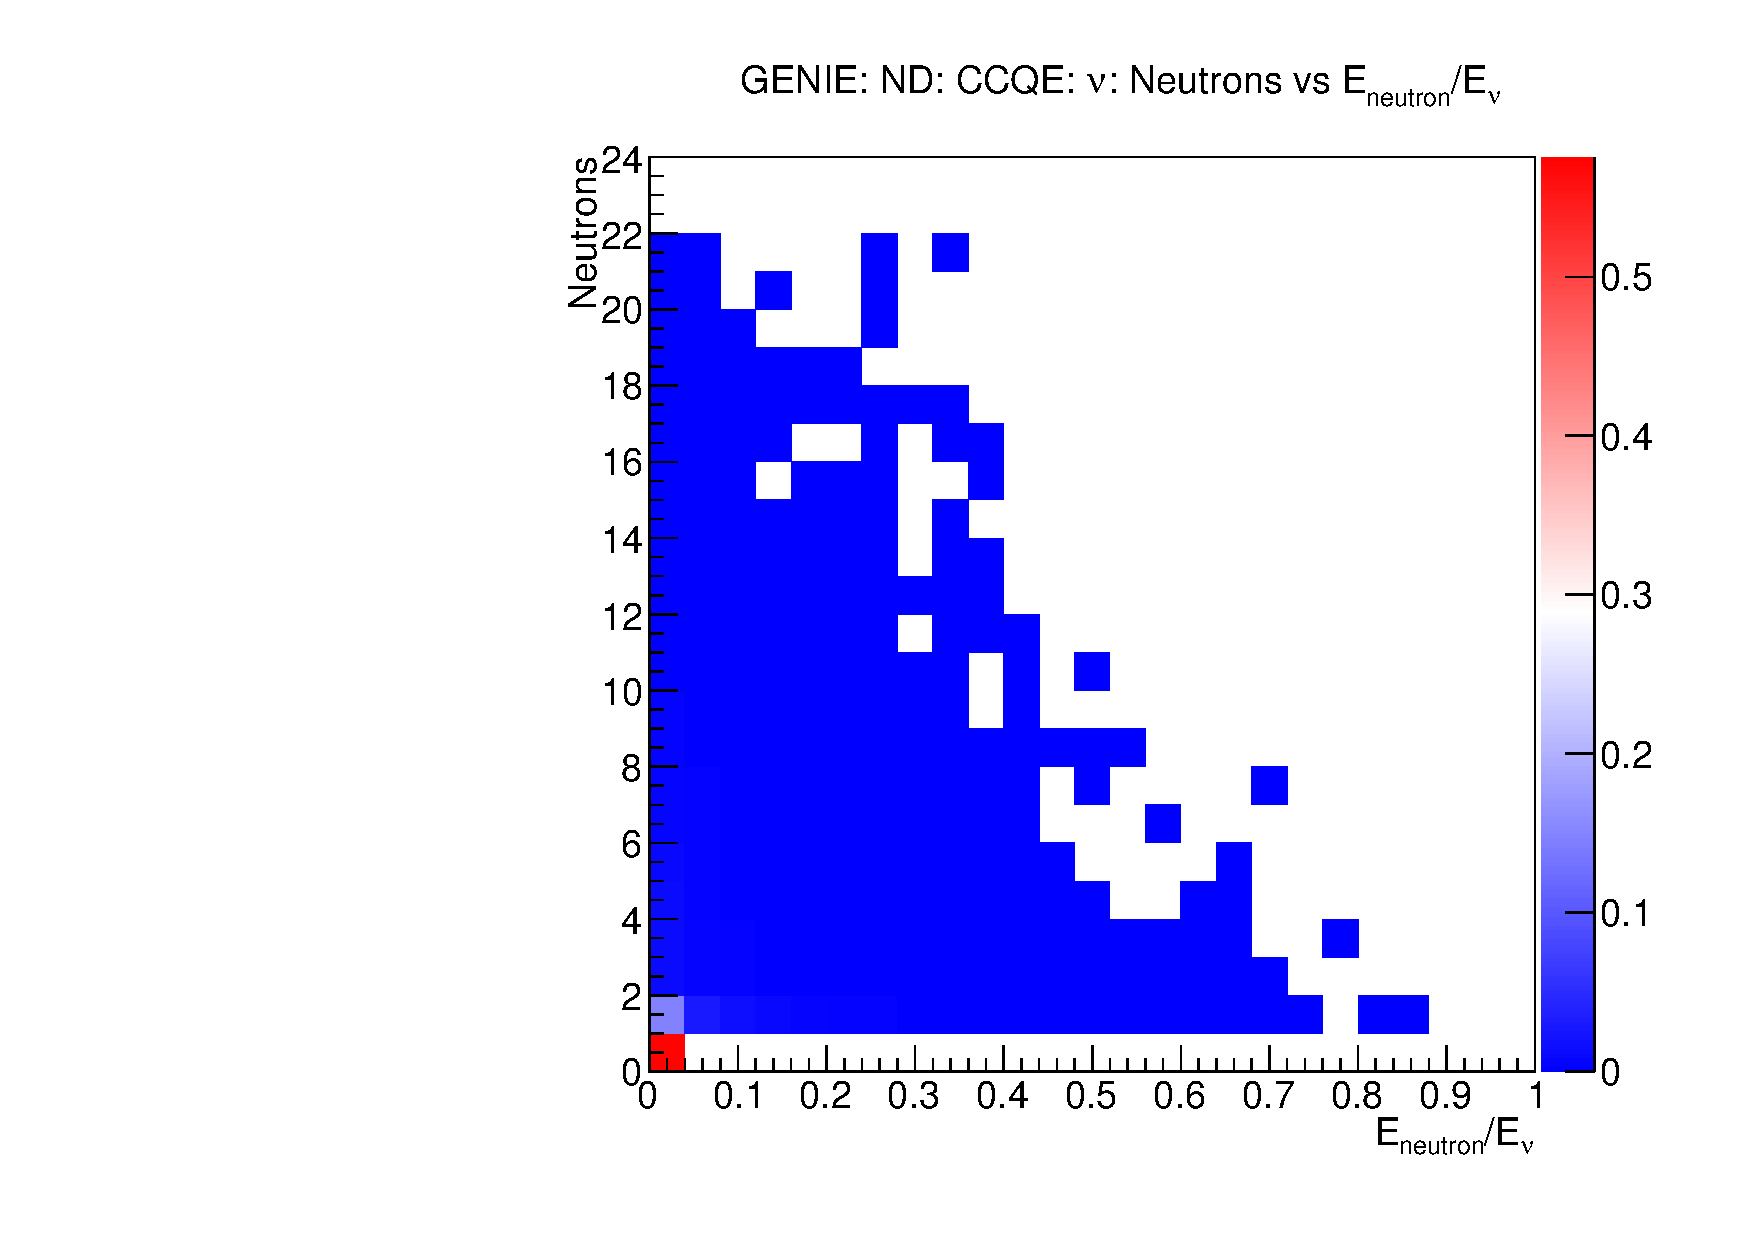
\includegraphics[width=\textwidth]{nneutrons_ene_enu/Nneutrons_Enu_true_ccqe_GENIE_ND_numu_norm.pdf}
\end{subfigure}
\begin{subfigure}[b]{0.32\textwidth}
  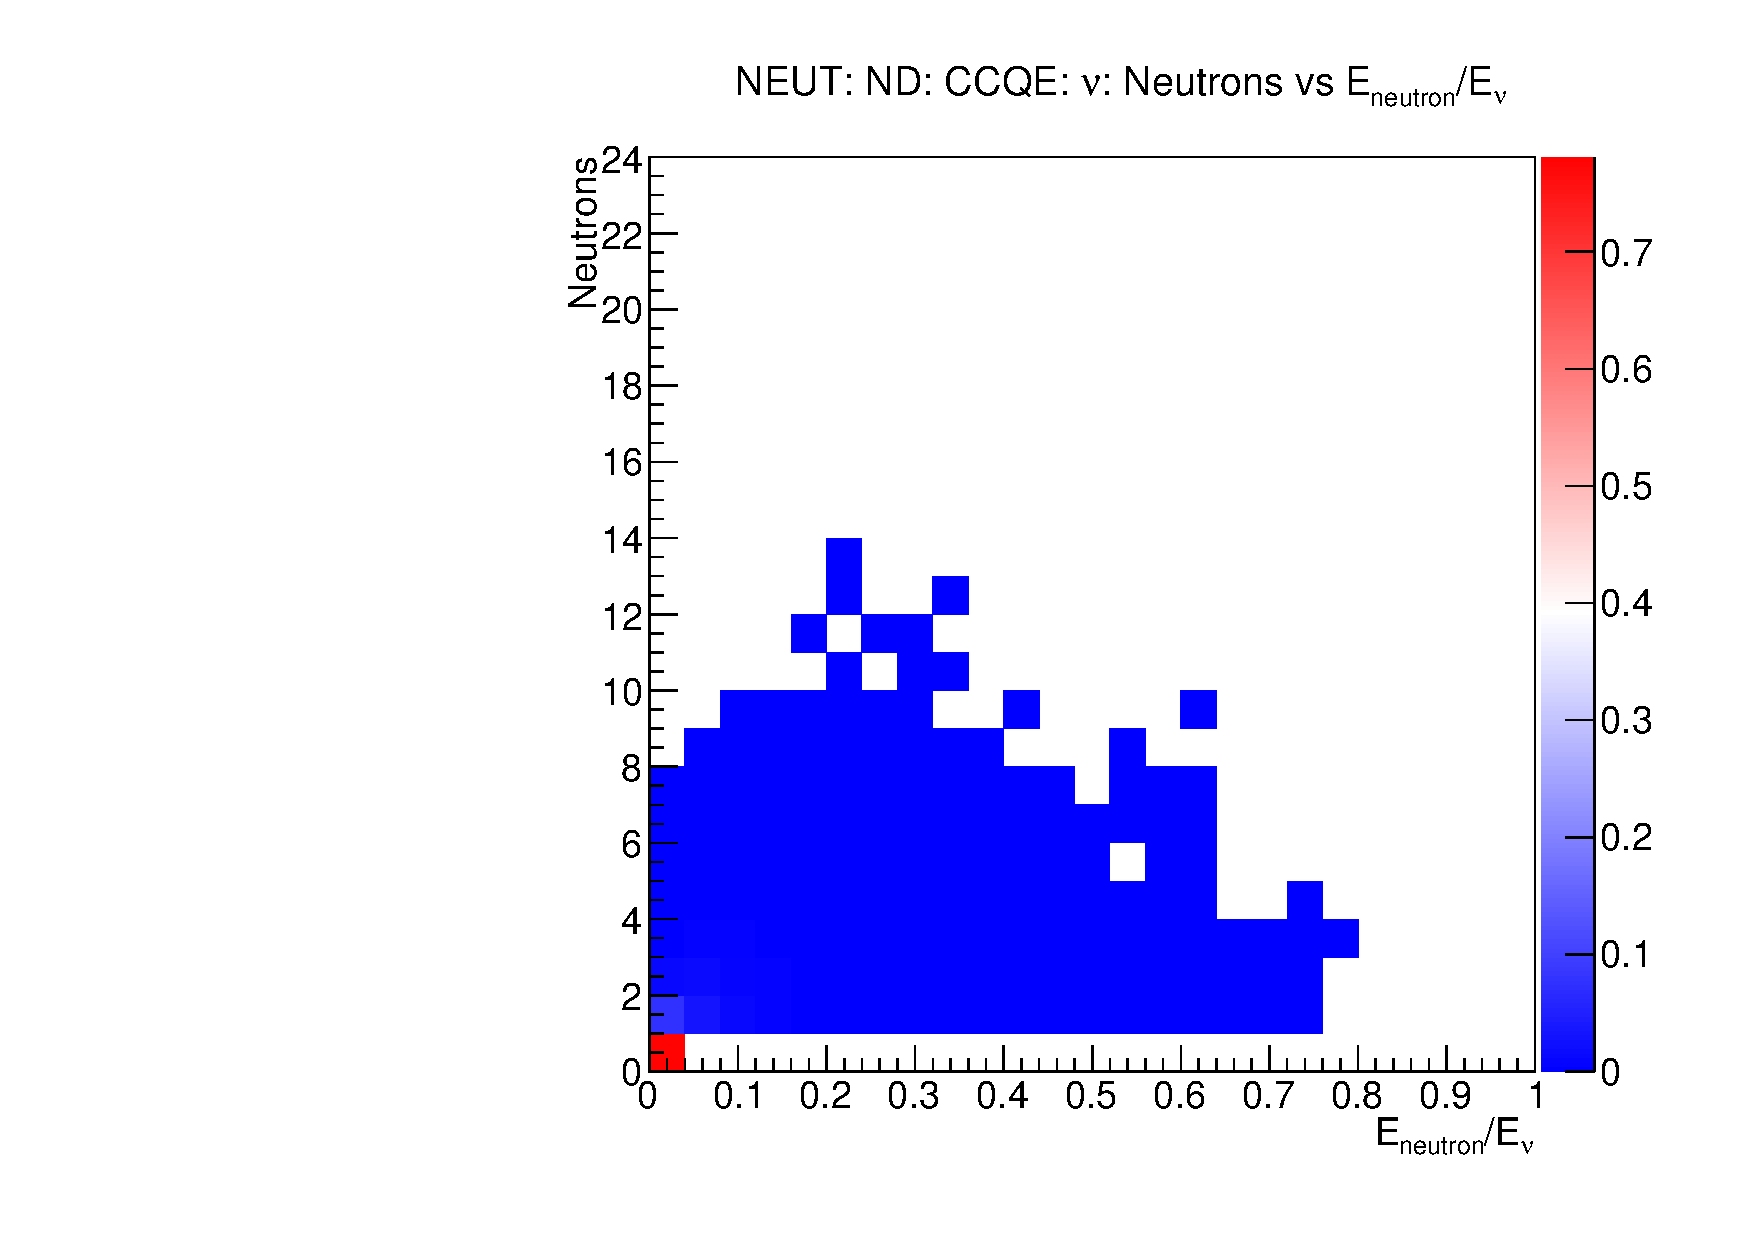
\includegraphics[width=\textwidth]{nneutrons_ene_enu/Nneutrons_Enu_true_ccqe_NEUT_ND_numu_norm.pdf}
\end{subfigure}
\begin{subfigure}[b]{0.32\textwidth}
  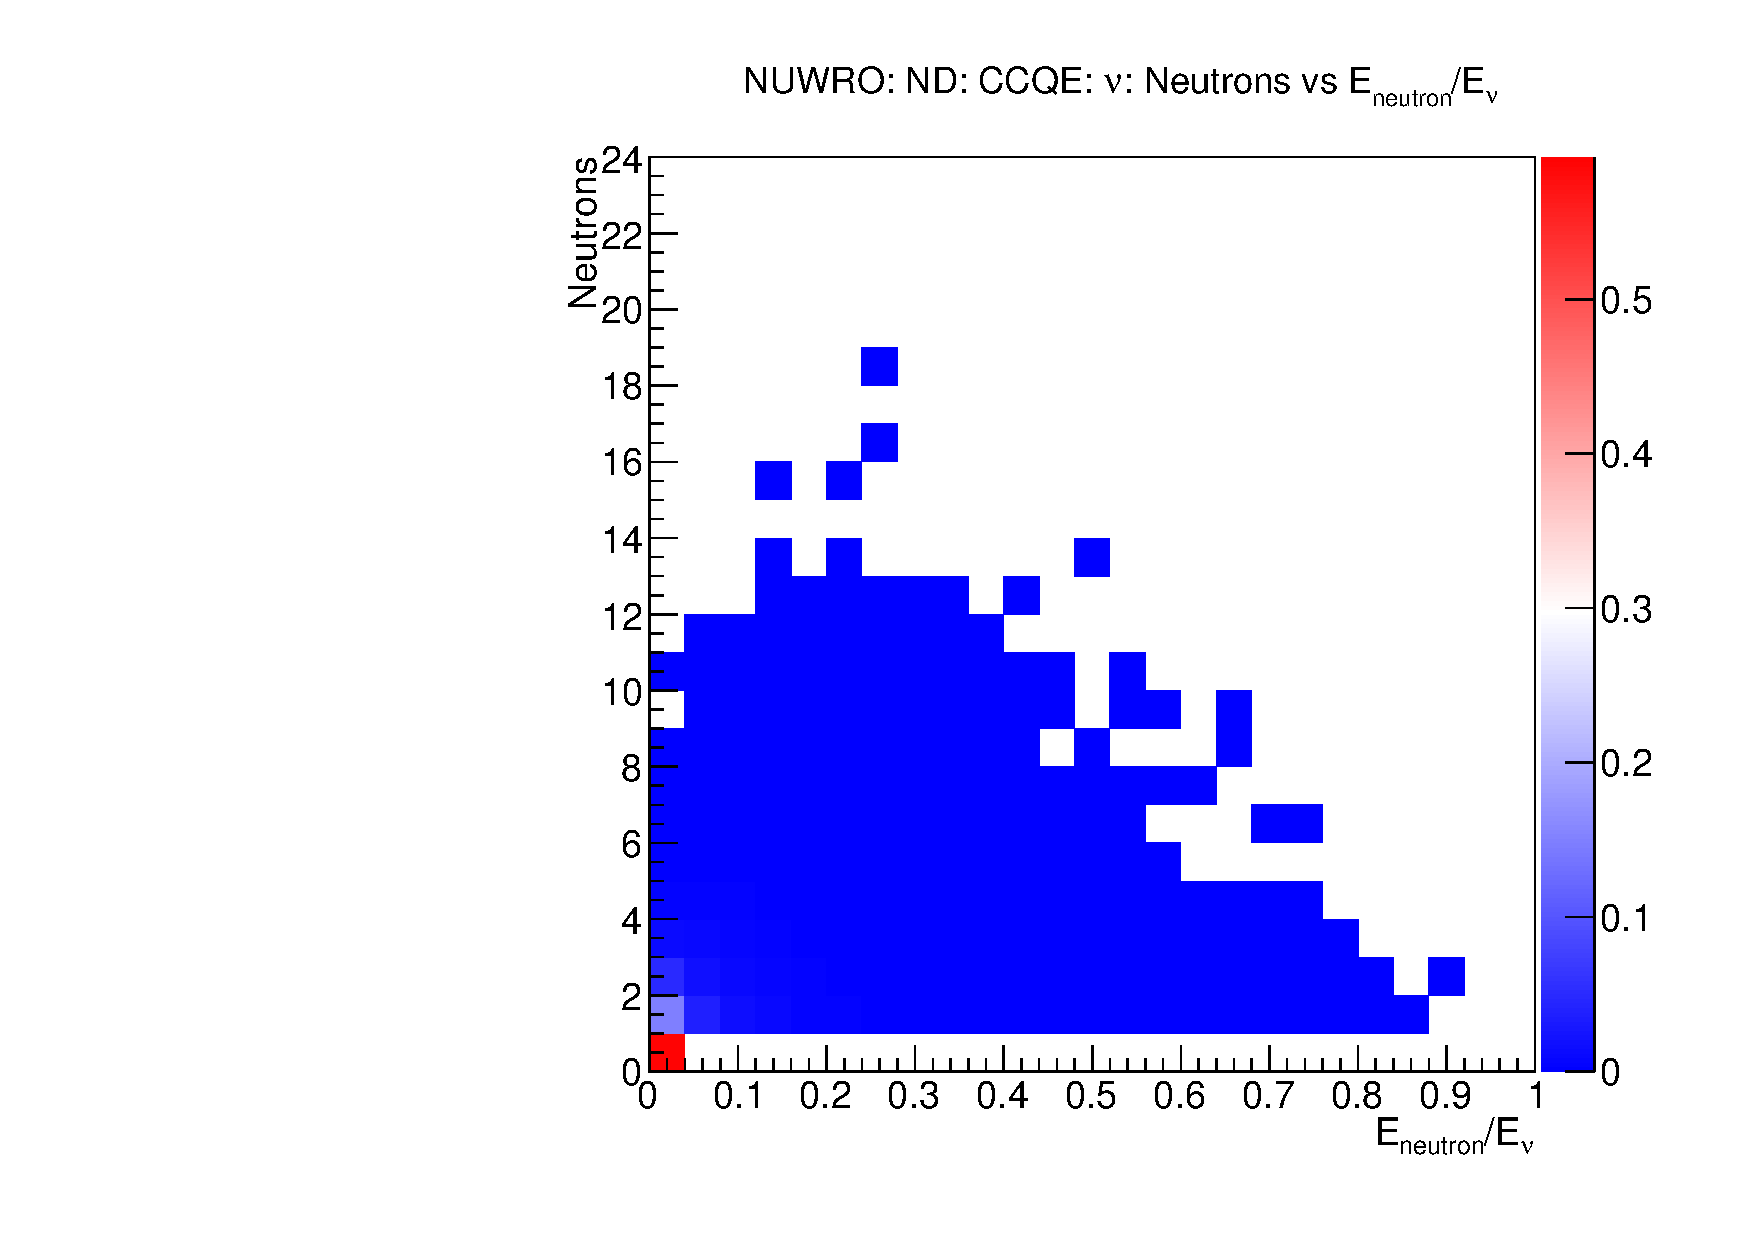
\includegraphics[width=\textwidth]{nneutrons_ene_enu/Nneutrons_Enu_true_ccqe_NUWRO_ND_numu_norm.pdf}
\end{subfigure}
\end{figure}
\FloatBarrier

\subsubsection{2P2H}

These are the same as shown in Section~\ref{subsec:N_multiplicities_Energy}. 

\begin{figure}[!htb]
\centering
\begin{subfigure}[b]{0.32\textwidth}
  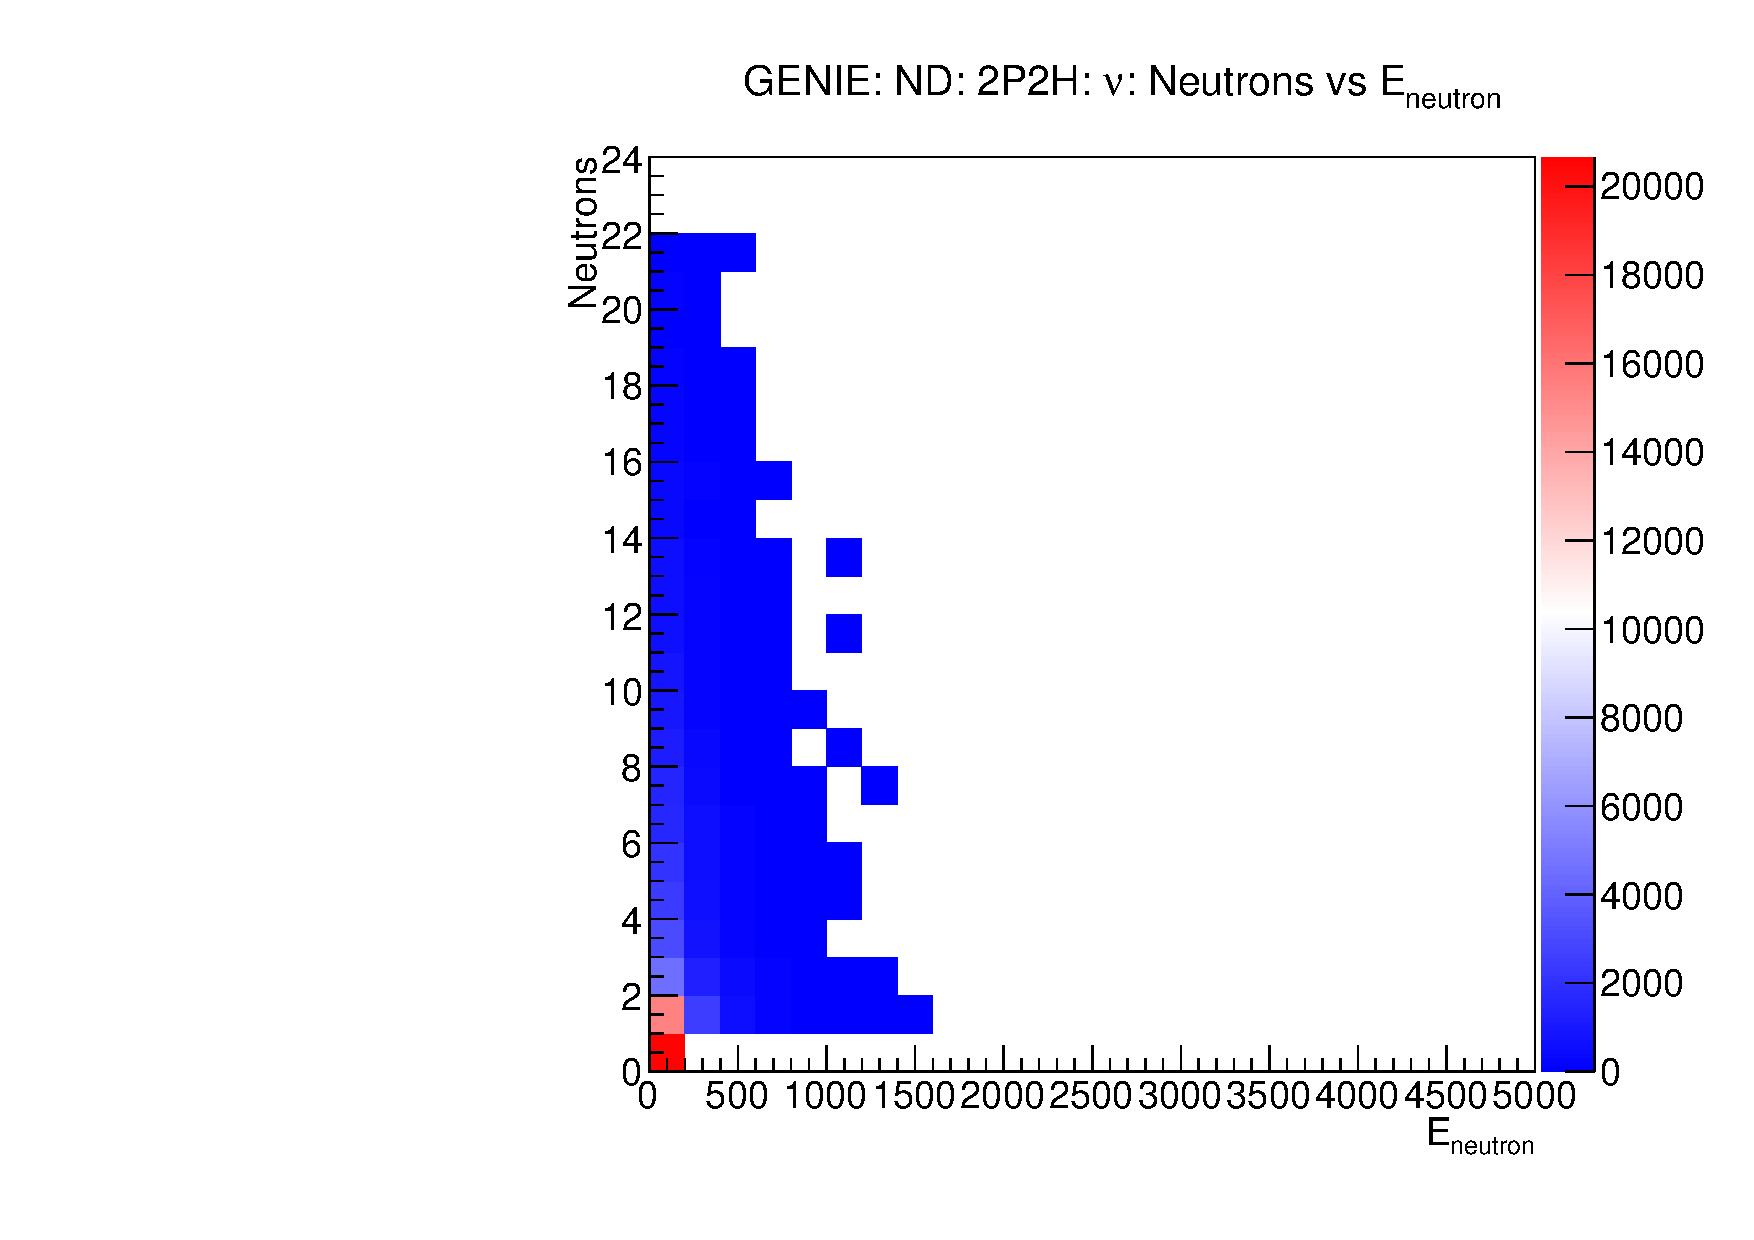
\includegraphics[width=\textwidth]{nneutrons_v_total_ene/Nneutrons_Total_ENe_2p2h_GENIE_ND_numu.pdf}
\end{subfigure}
\begin{subfigure}[b]{0.32\textwidth}
  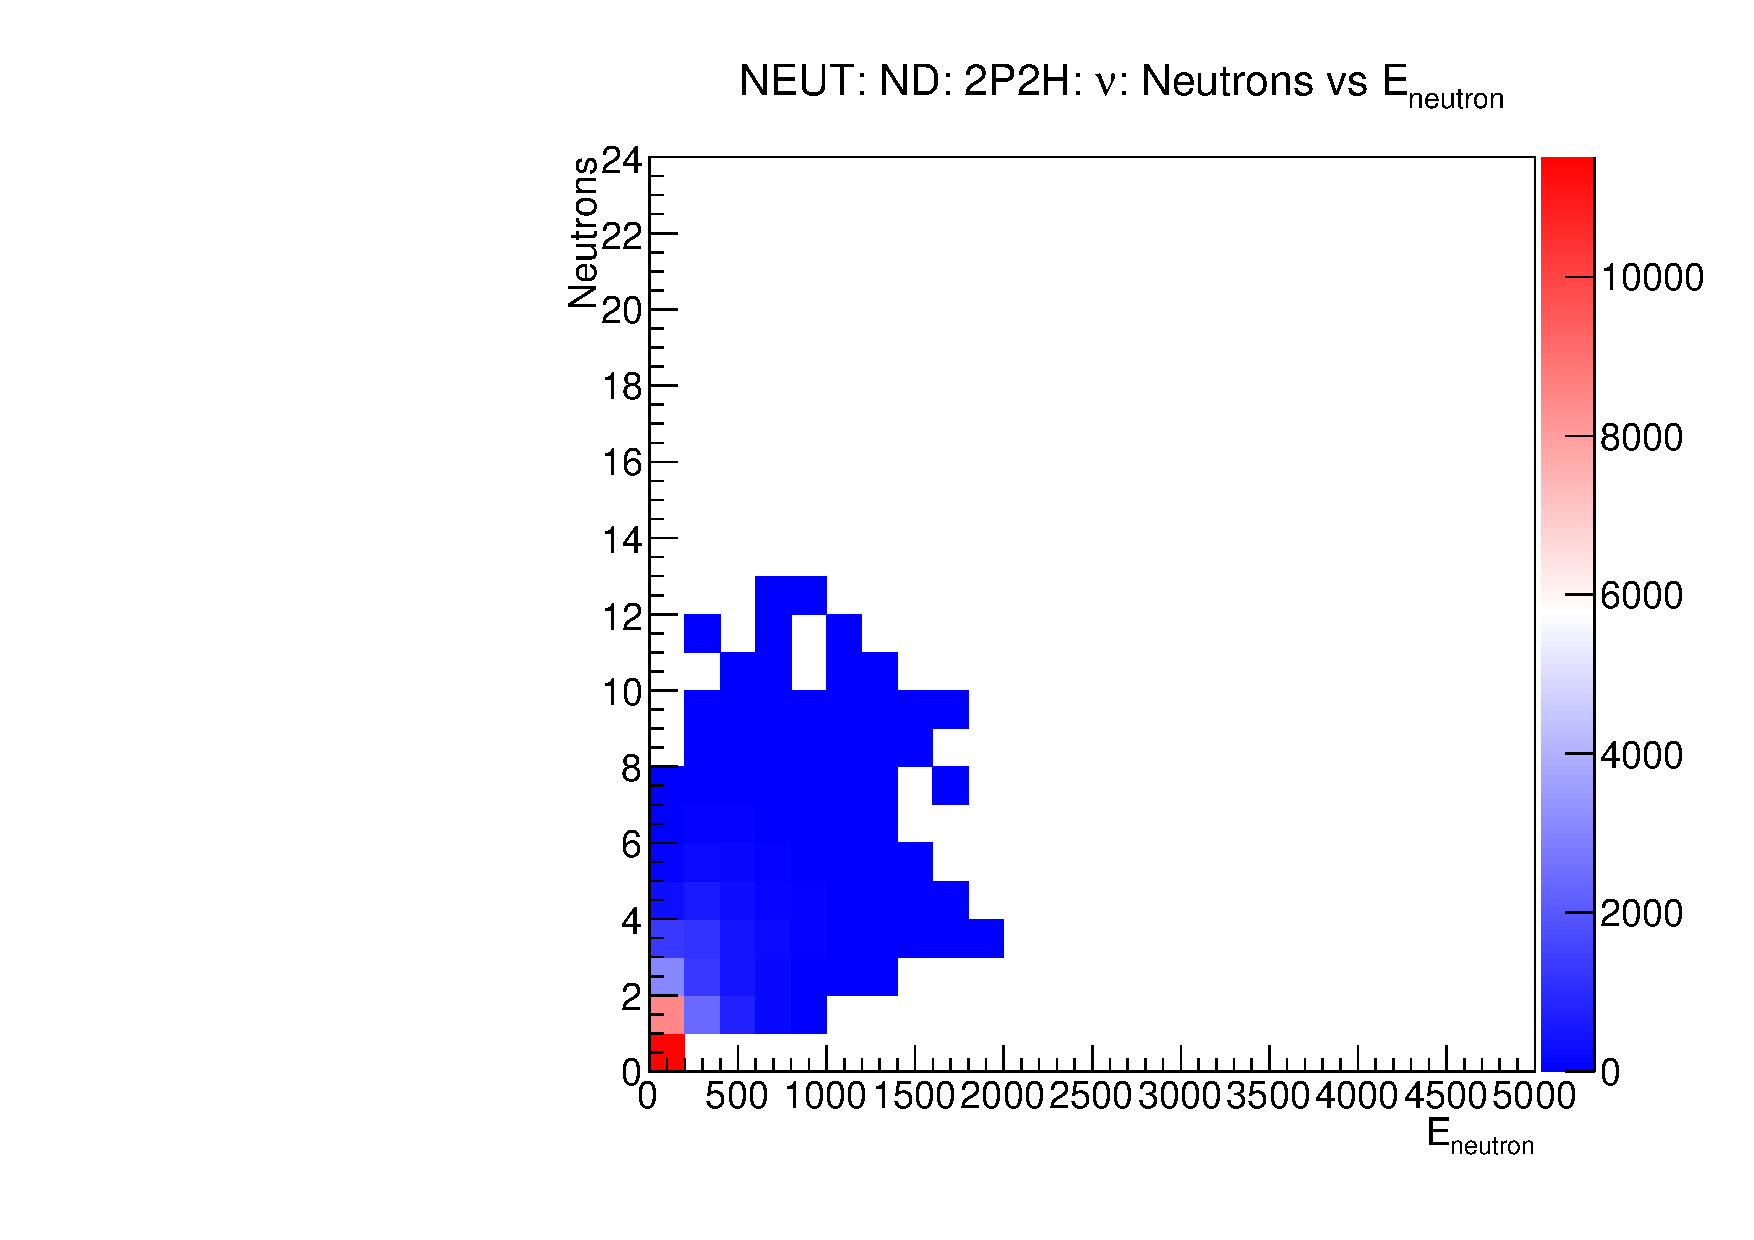
\includegraphics[width=\textwidth]{nneutrons_v_total_ene/Nneutrons_Total_ENe_2p2h_NEUT_ND_numu.pdf}
\end{subfigure}
\begin{subfigure}[b]{0.32\textwidth}
  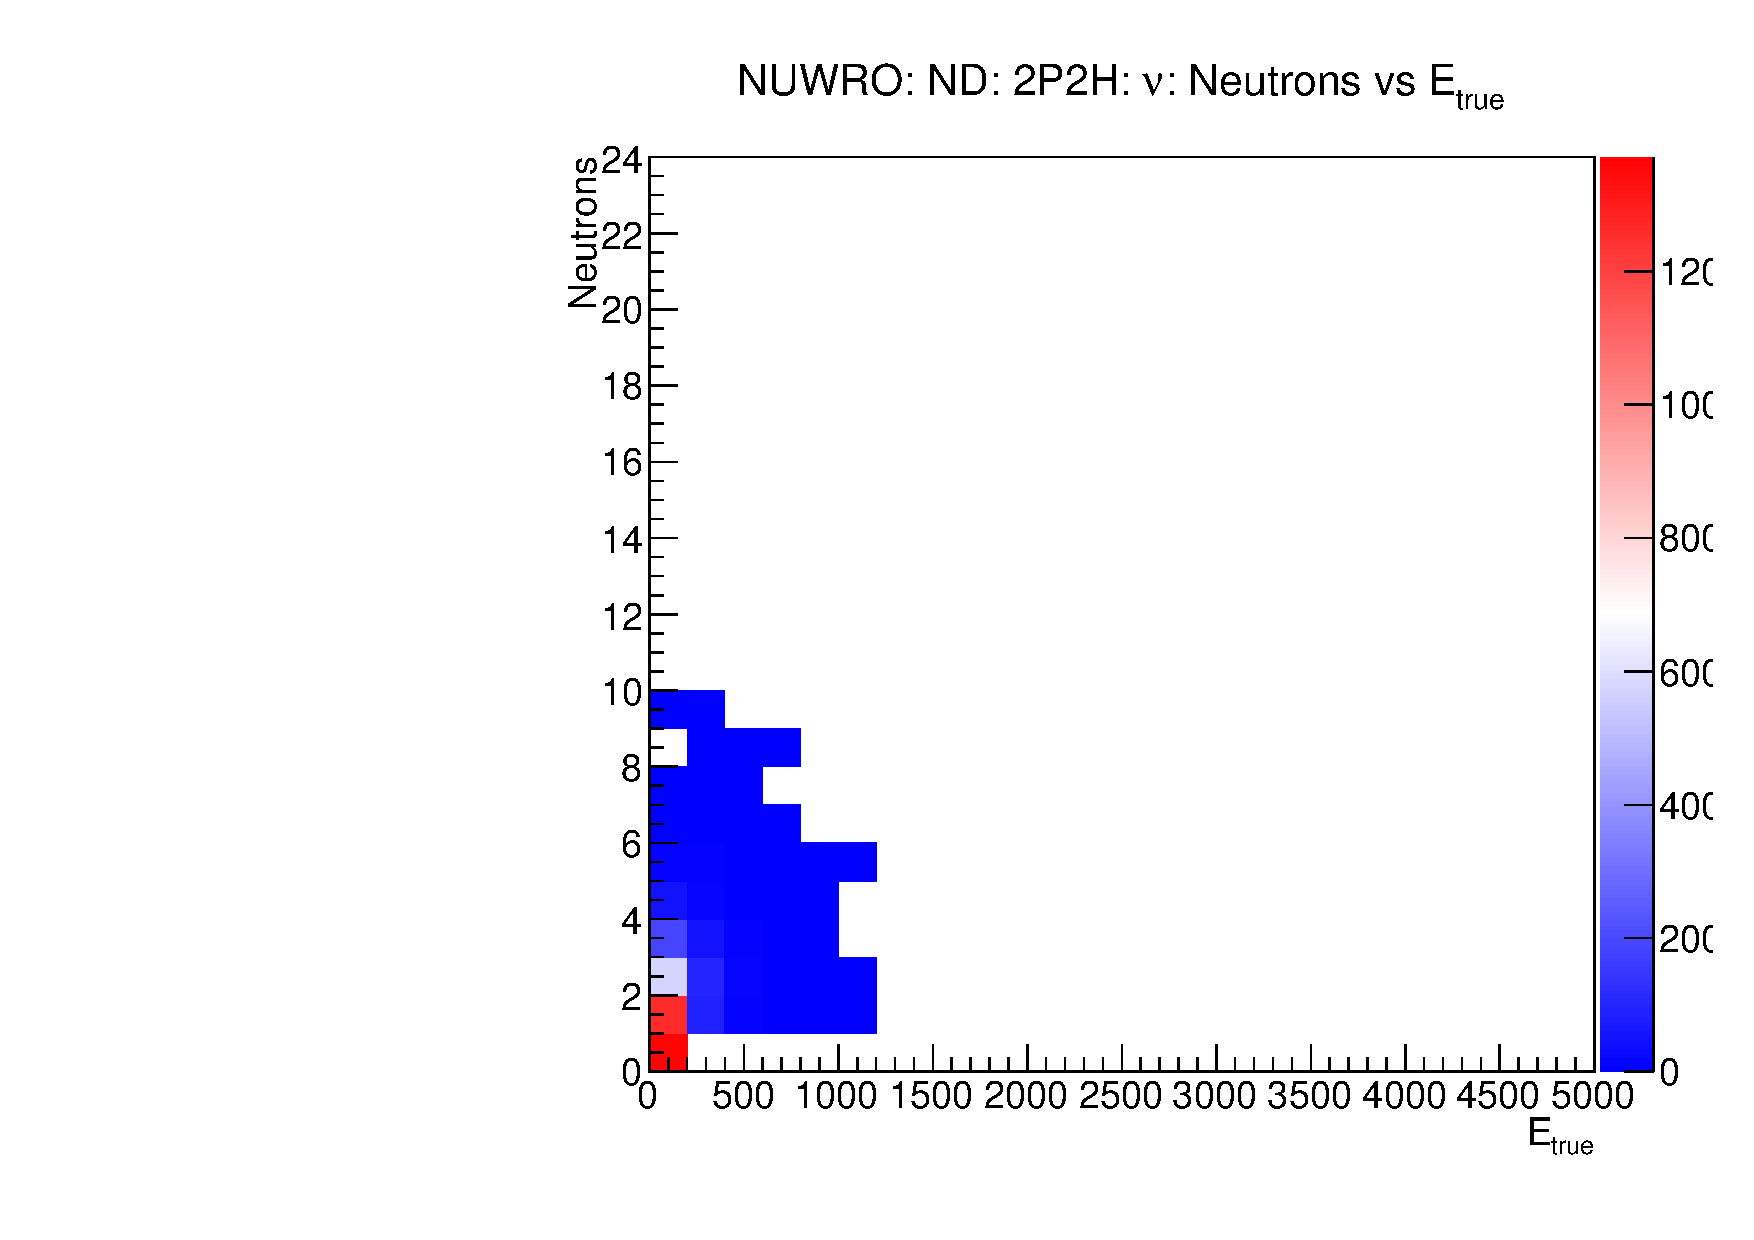
\includegraphics[width=\textwidth]{nneutrons_v_total_ene/Nneutrons_Total_ENe_2p2h_NUWRO_ND_numu.pdf}
\end{subfigure}
\end{figure}

\begin{figure}[!htb]
\centering
\begin{subfigure}[b]{0.32\textwidth}
  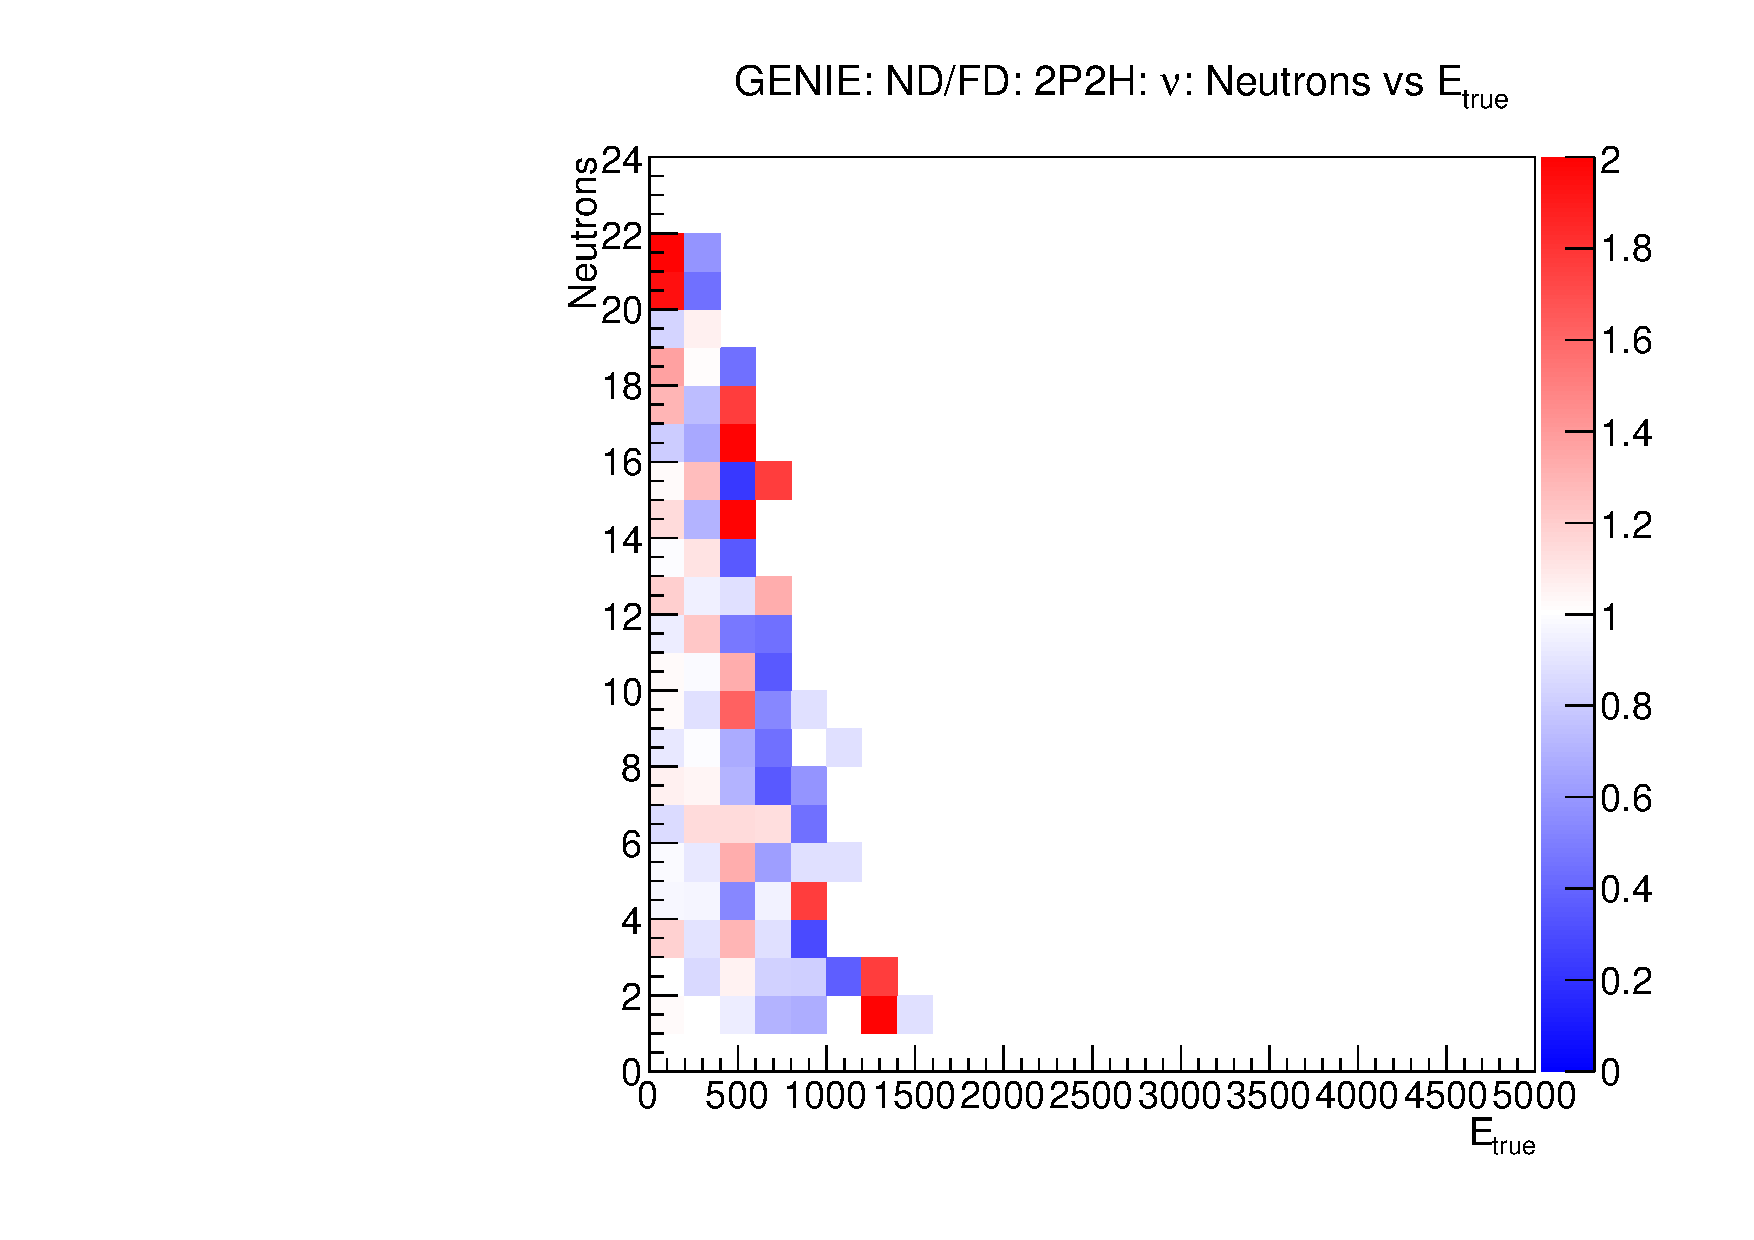
\includegraphics[width=\textwidth]{nneutrons_v_total_ene/Nneutrons_Total_ENe_2p2h_GENIE_ND_FD_numu_norm.pdf}
\end{subfigure}
\begin{subfigure}[b]{0.32\textwidth}
  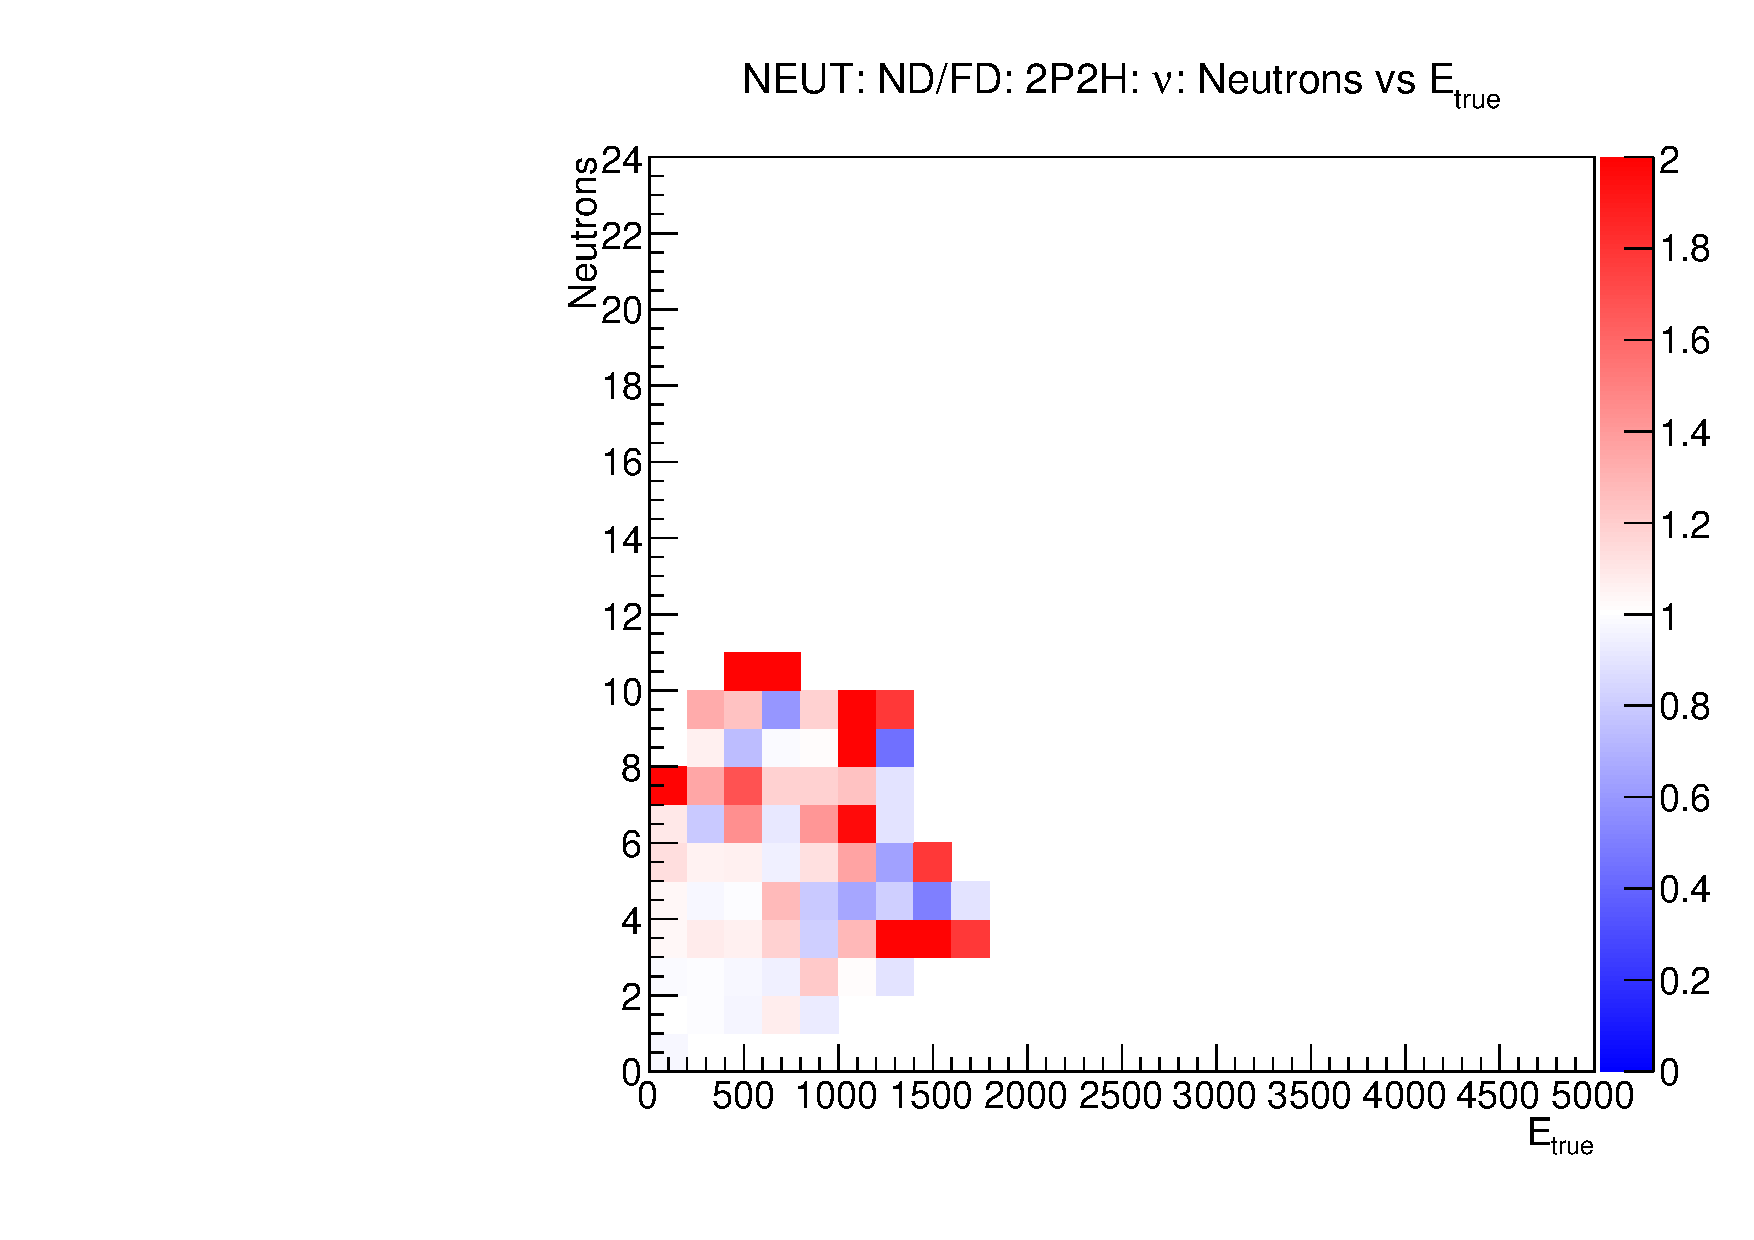
\includegraphics[width=\textwidth]{nneutrons_v_total_ene/Nneutrons_Total_ENe_2p2h_NEUT_ND_FD_numu_norm.pdf}
\end{subfigure}
\begin{subfigure}[b]{0.32\textwidth}
  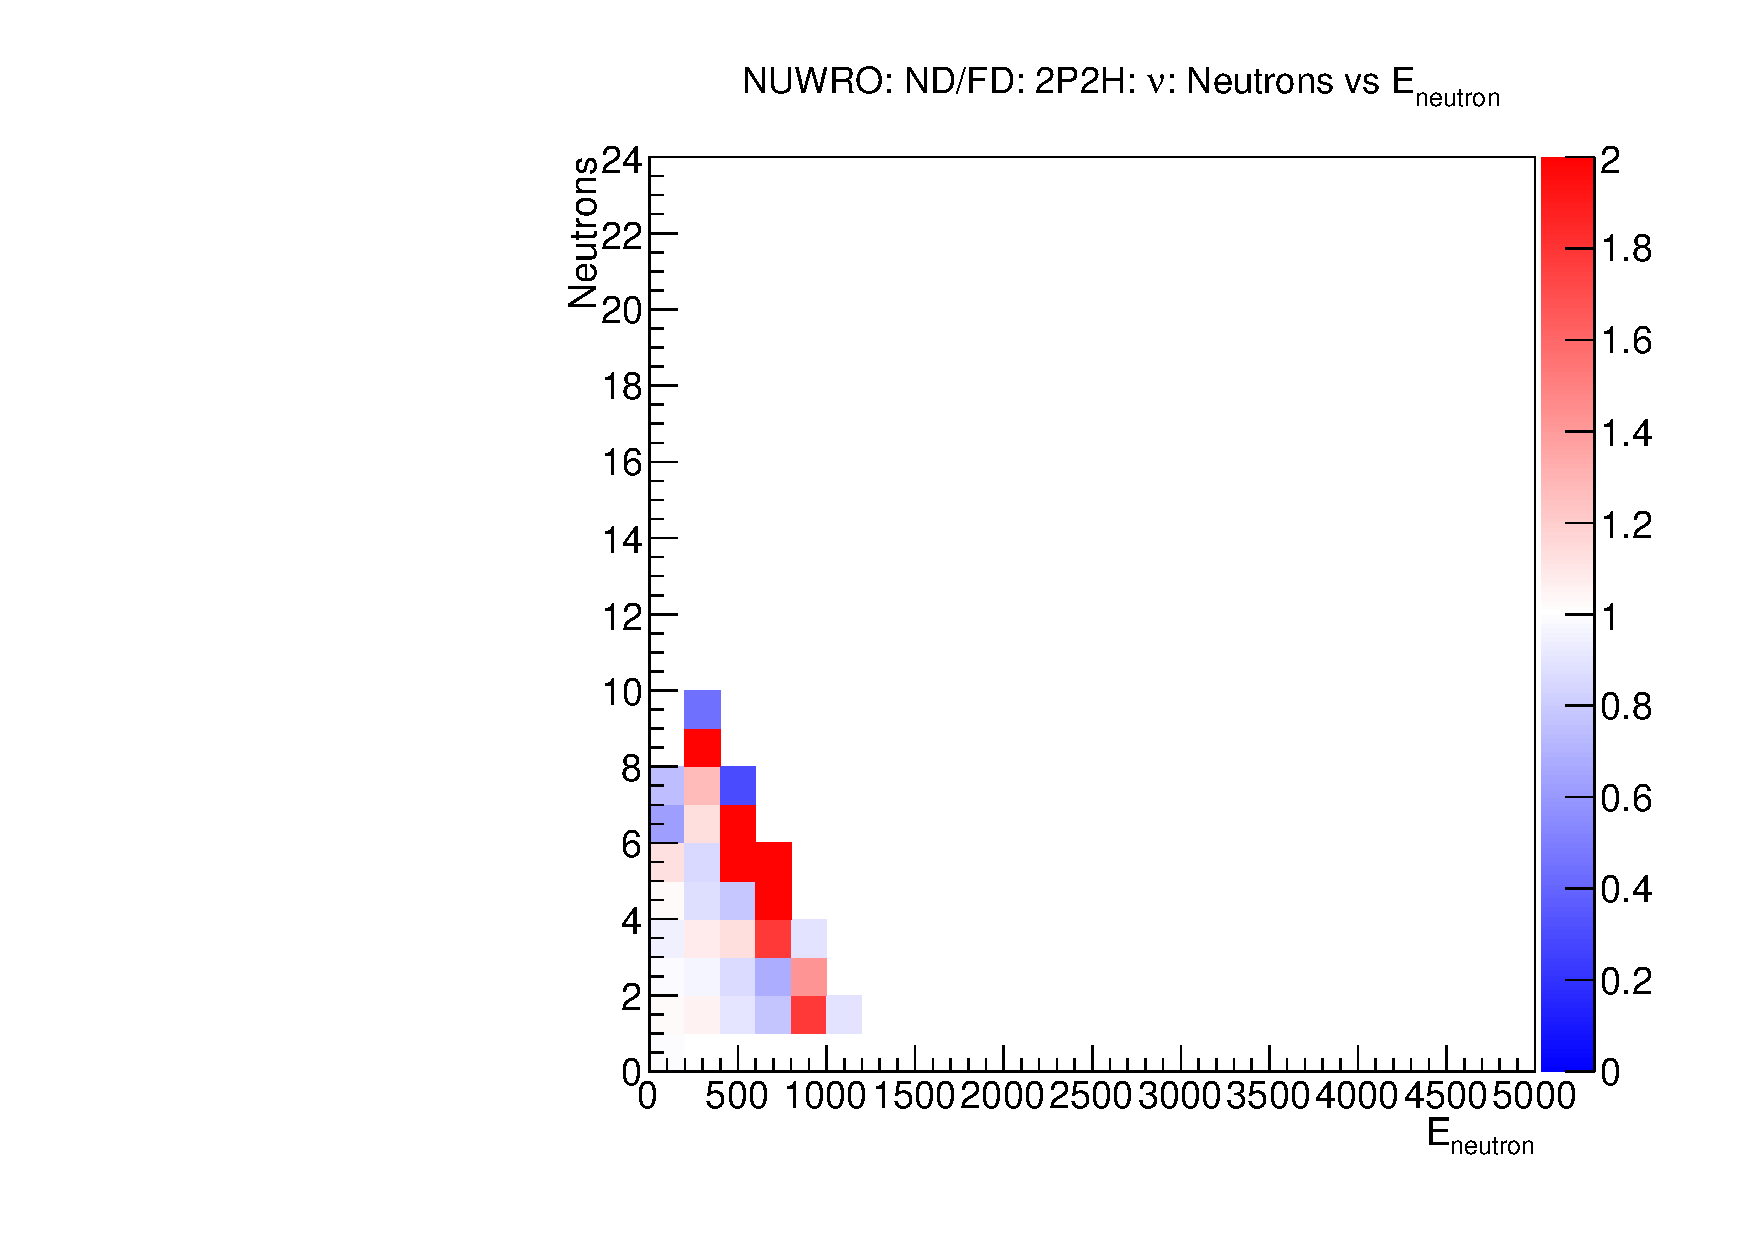
\includegraphics[width=\textwidth]{nneutrons_v_total_ene/Nneutrons_Total_ENe_2p2h_NUWRO_ND_FD_numu_norm.pdf}
\end{subfigure}
\end{figure}

\begin{figure}[!htb]
\centering
\begin{subfigure}[b]{0.32\textwidth}
  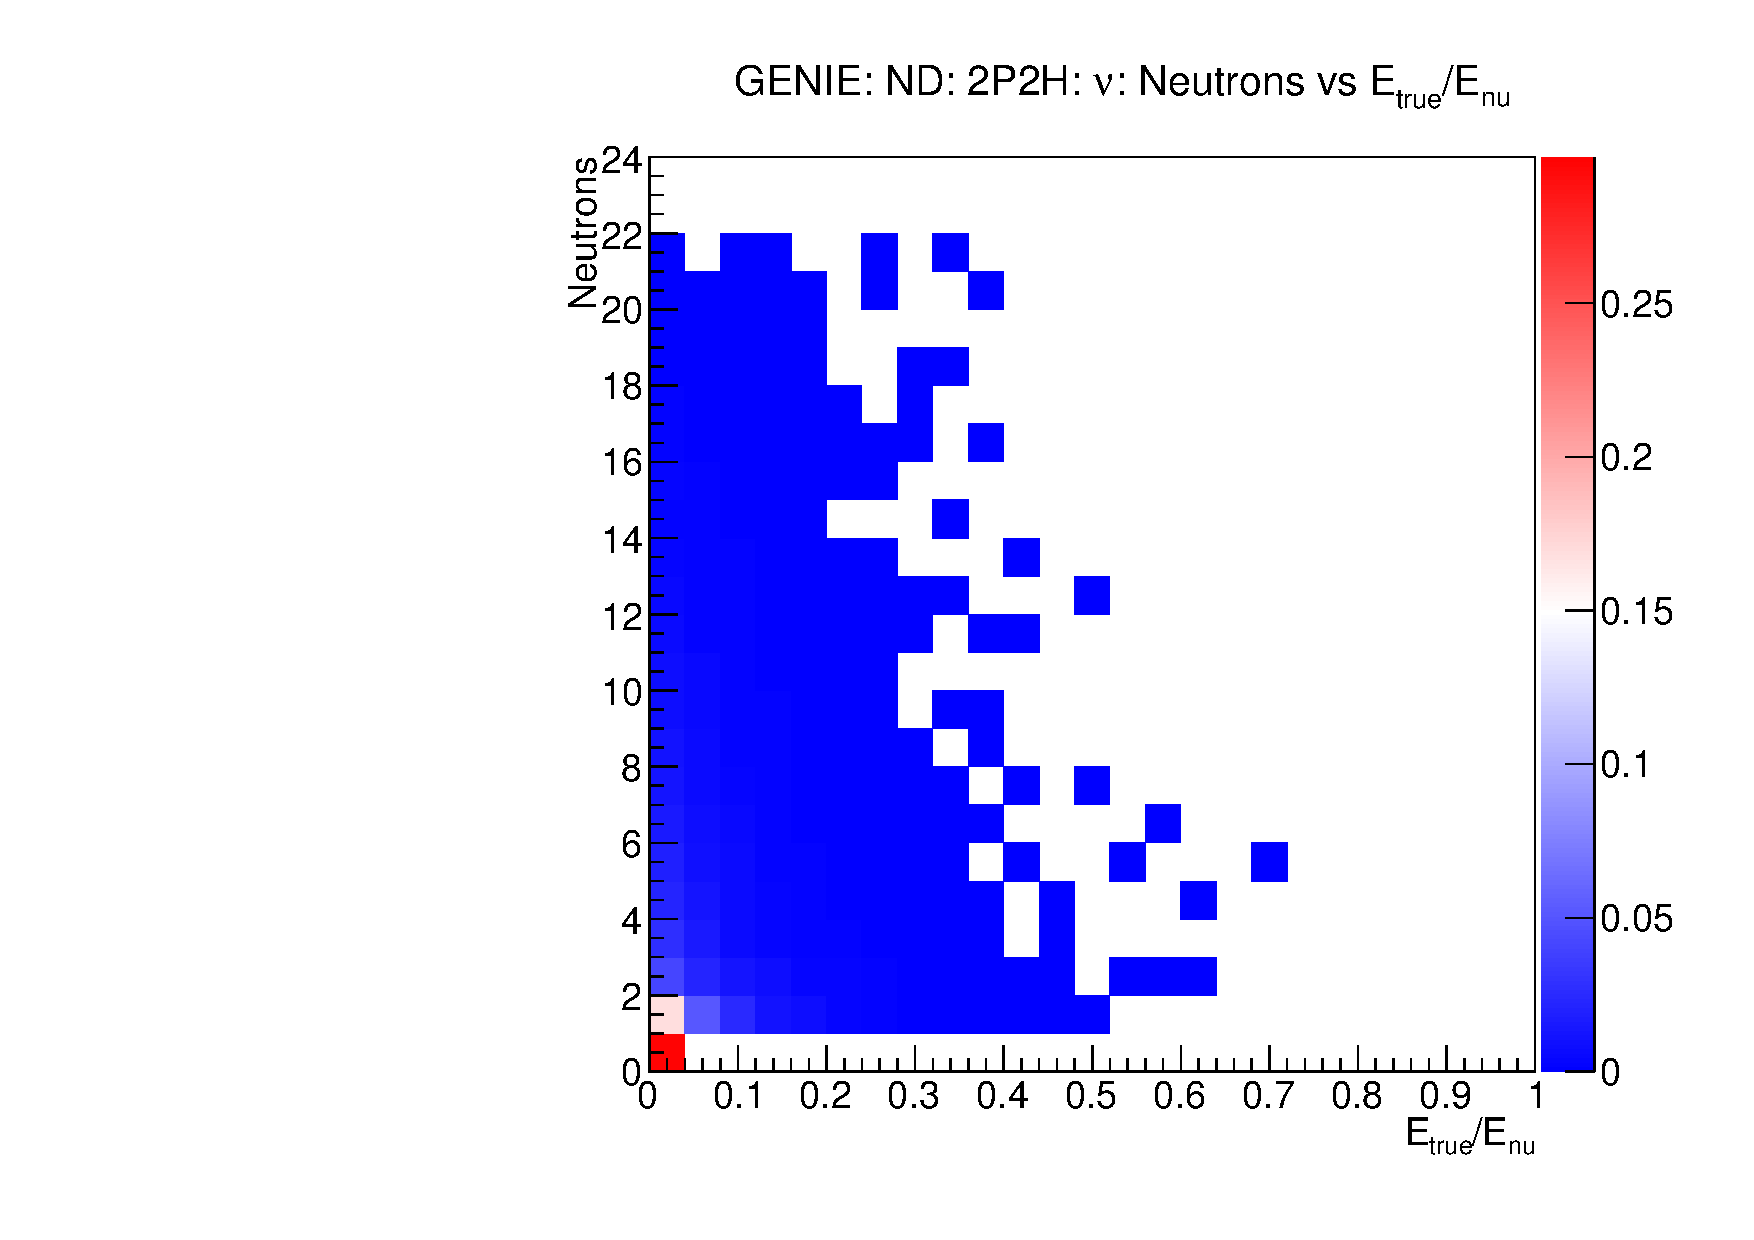
\includegraphics[width=\textwidth]{nneutrons_ene_enu/Nneutrons_Enu_true_2p2h_GENIE_ND_numu_norm.pdf}
\end{subfigure}
\begin{subfigure}[b]{0.32\textwidth}
  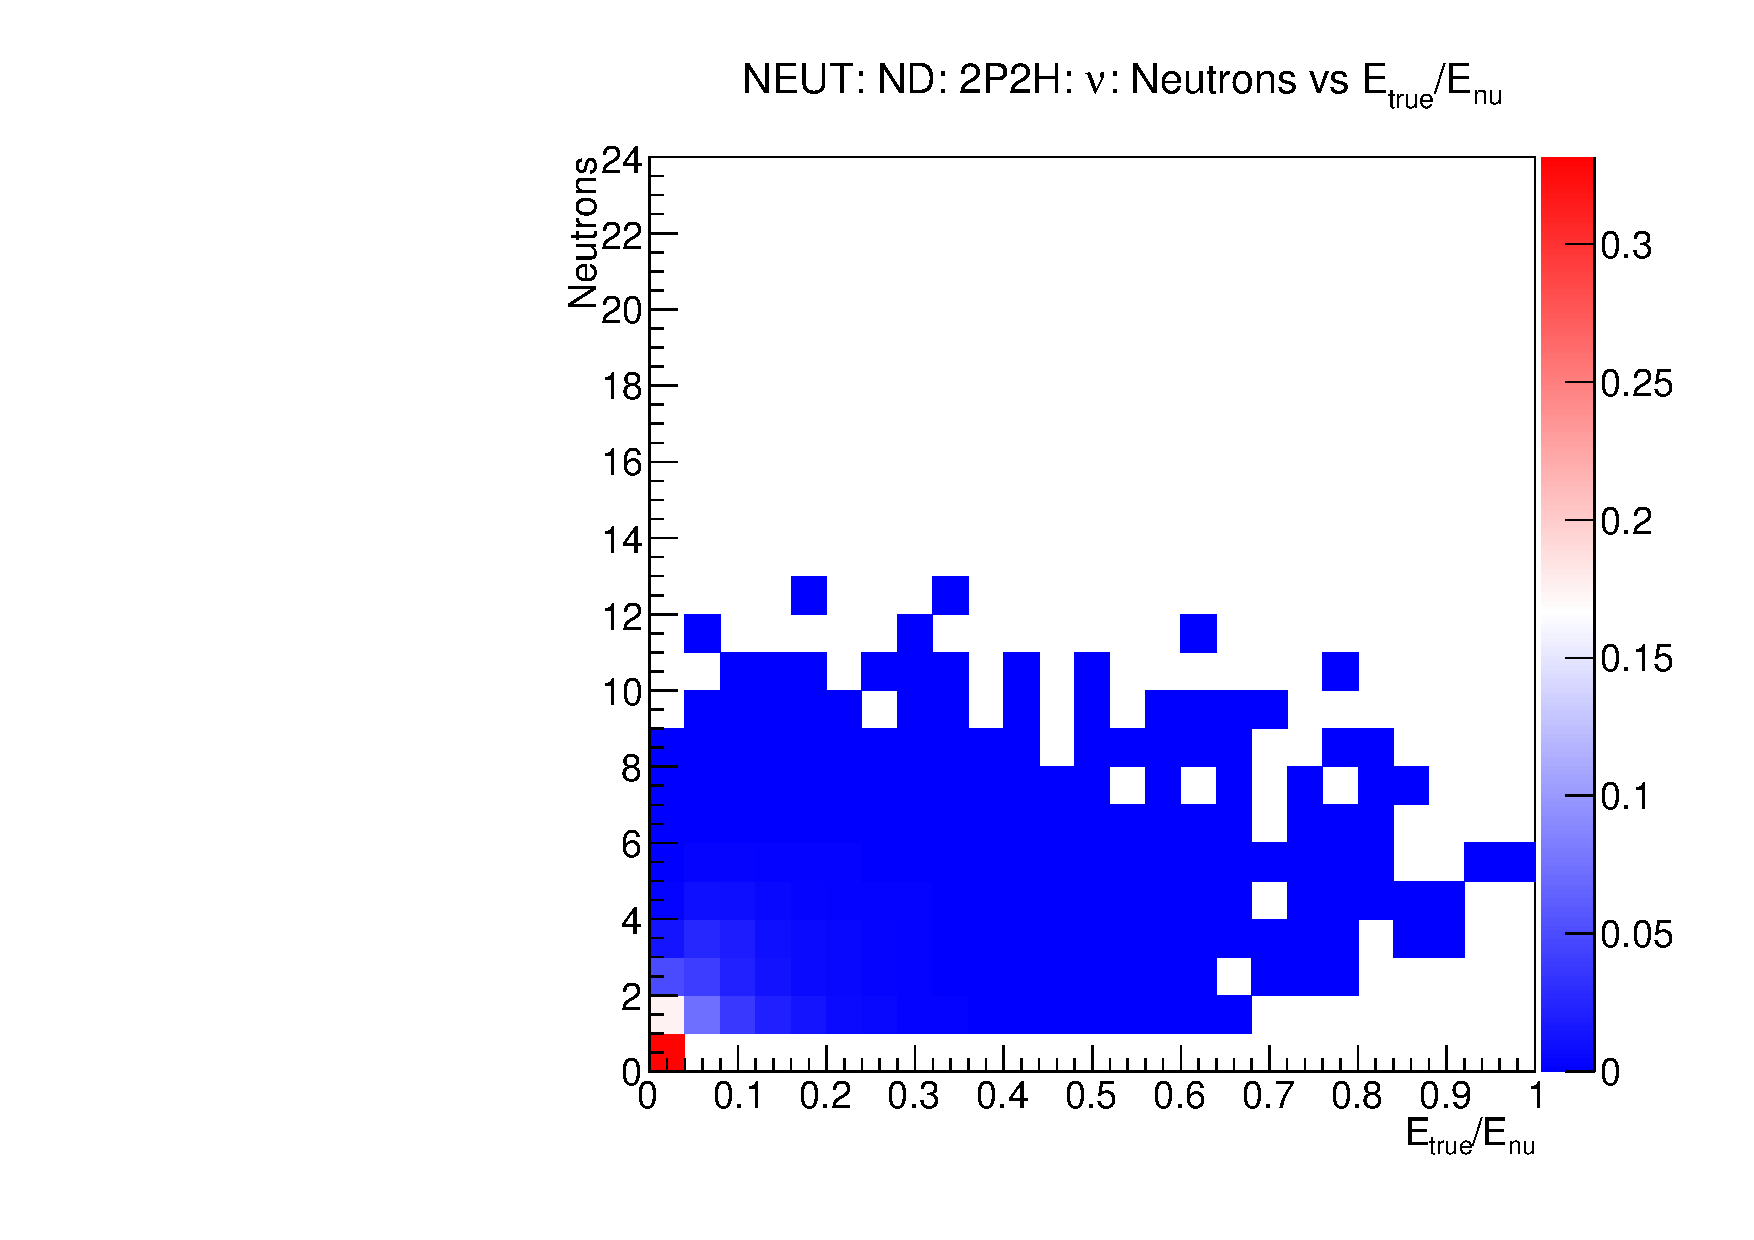
\includegraphics[width=\textwidth]{nneutrons_ene_enu/Nneutrons_Enu_true_2p2h_NEUT_ND_numu_norm.pdf}
\end{subfigure}
\begin{subfigure}[b]{0.32\textwidth}
  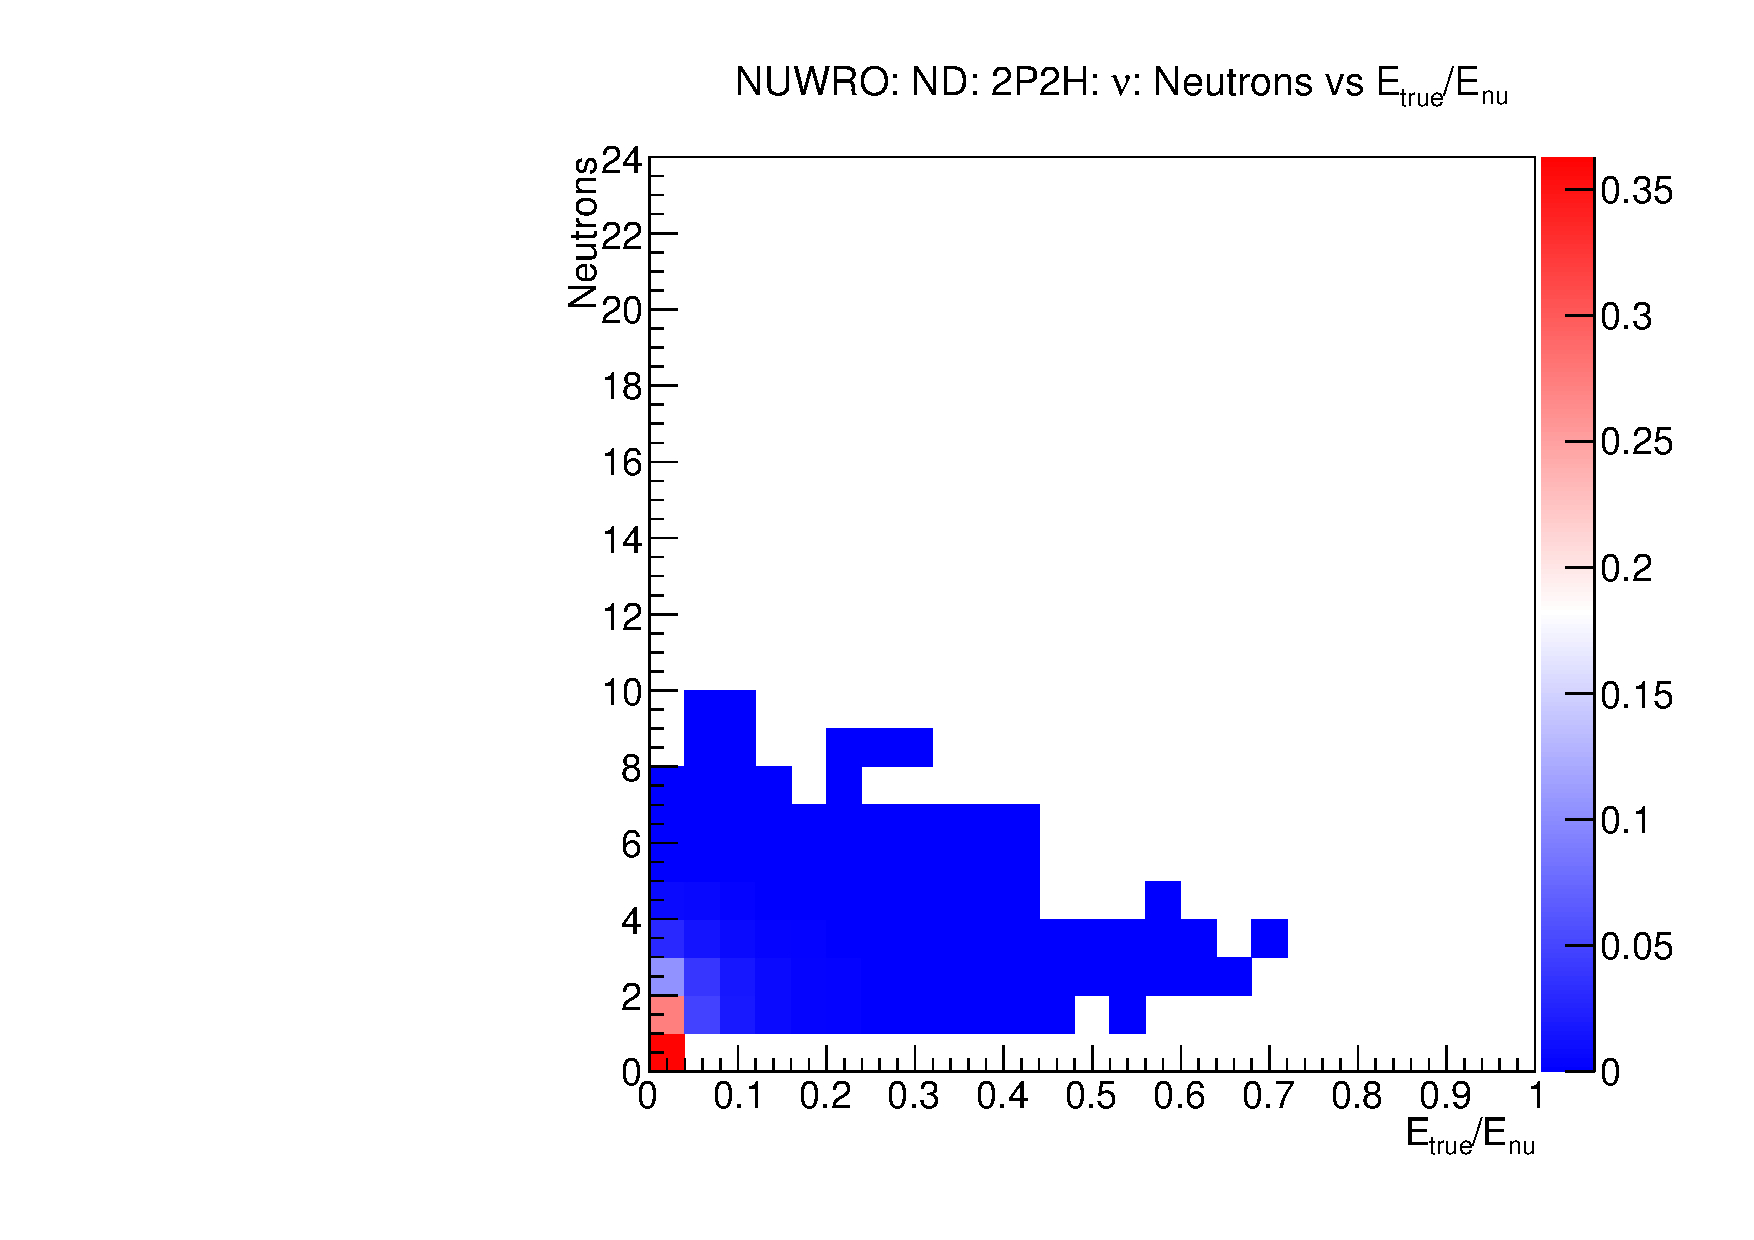
\includegraphics[width=\textwidth]{nneutrons_ene_enu/Nneutrons_Enu_true_2p2h_NUWRO_ND_numu_norm.pdf}
\end{subfigure}
\end{figure}
\FloatBarrier

\subsubsection{CC1$\pi$}

\begin{figure}[!htb]
\centering
\begin{subfigure}[b]{0.32\textwidth}
  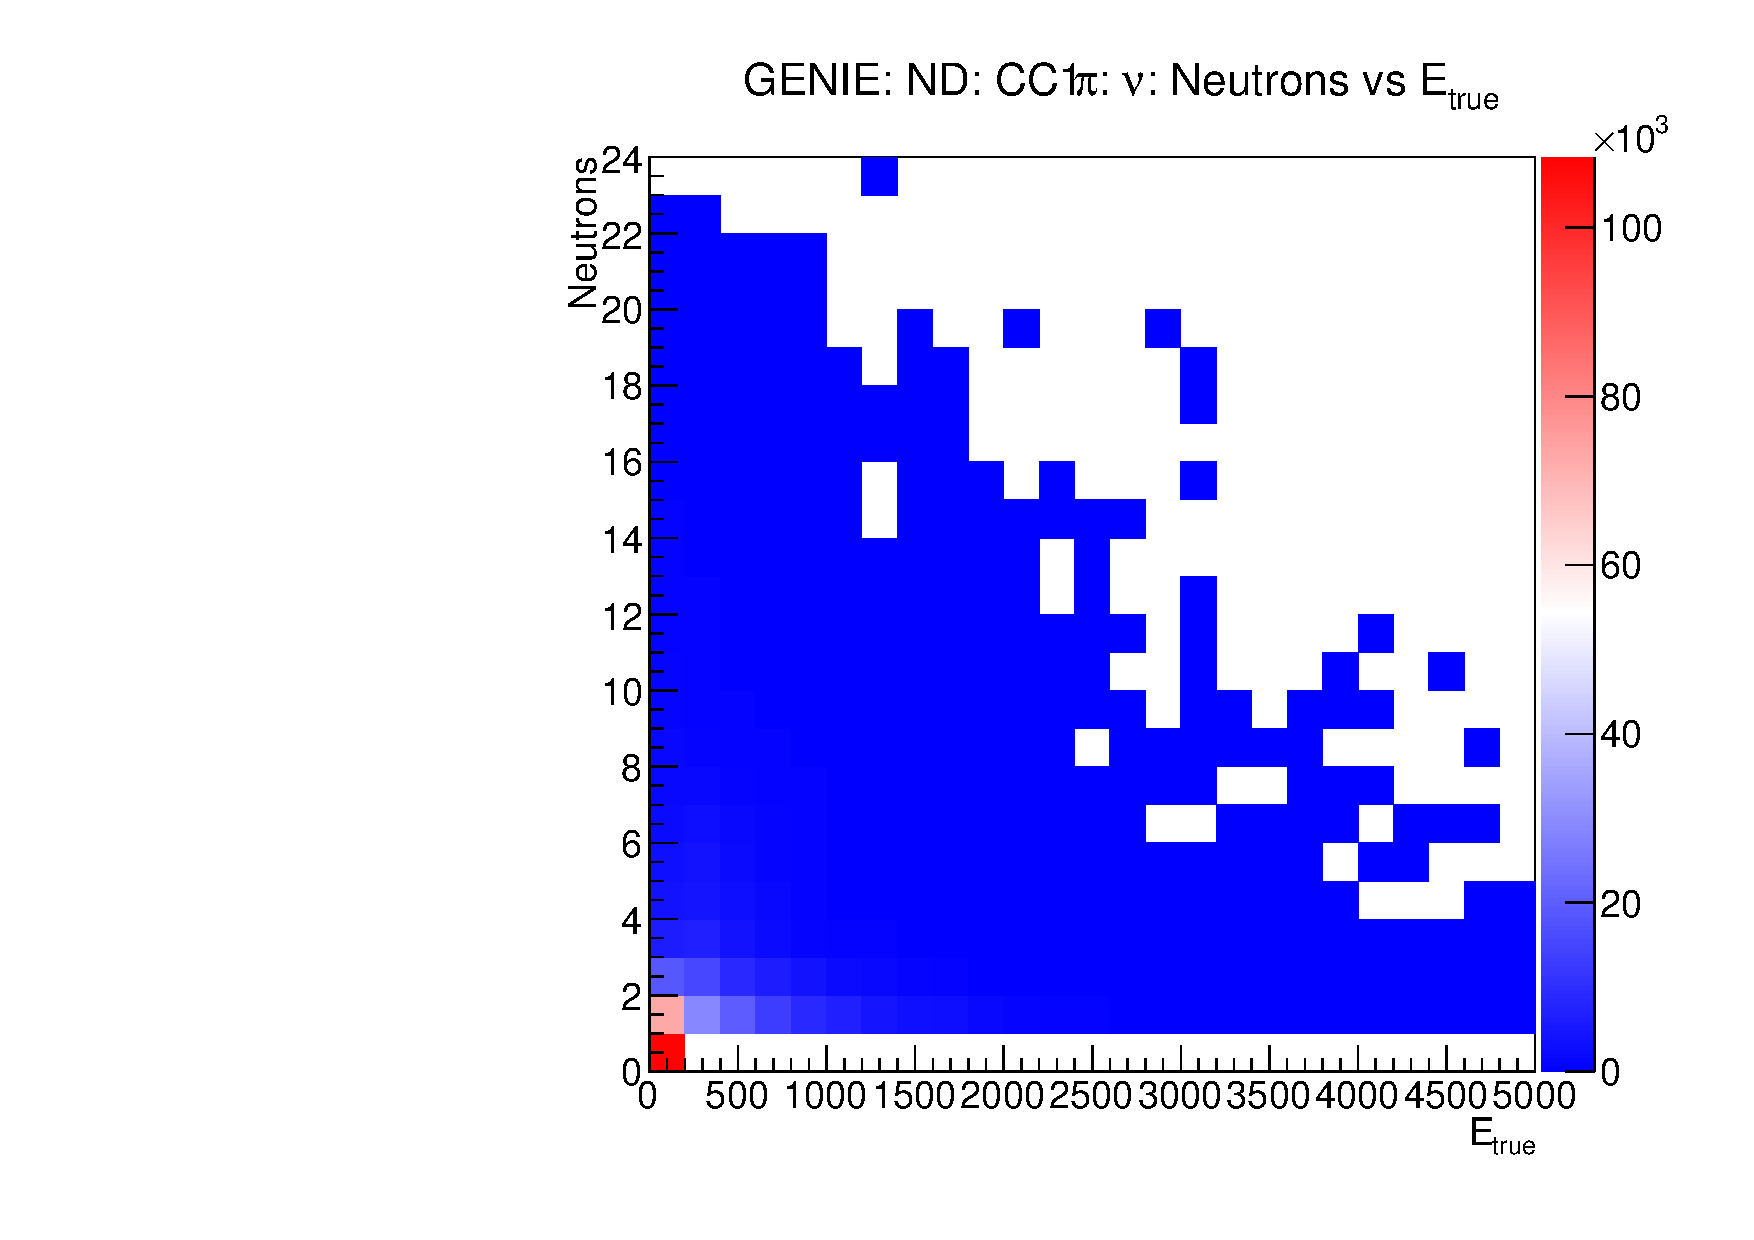
\includegraphics[width=\textwidth]{nneutrons_v_total_ene/Nneutrons_Total_ENe_res_GENIE_ND_numu.pdf}
\end{subfigure}
\begin{subfigure}[b]{0.32\textwidth}
  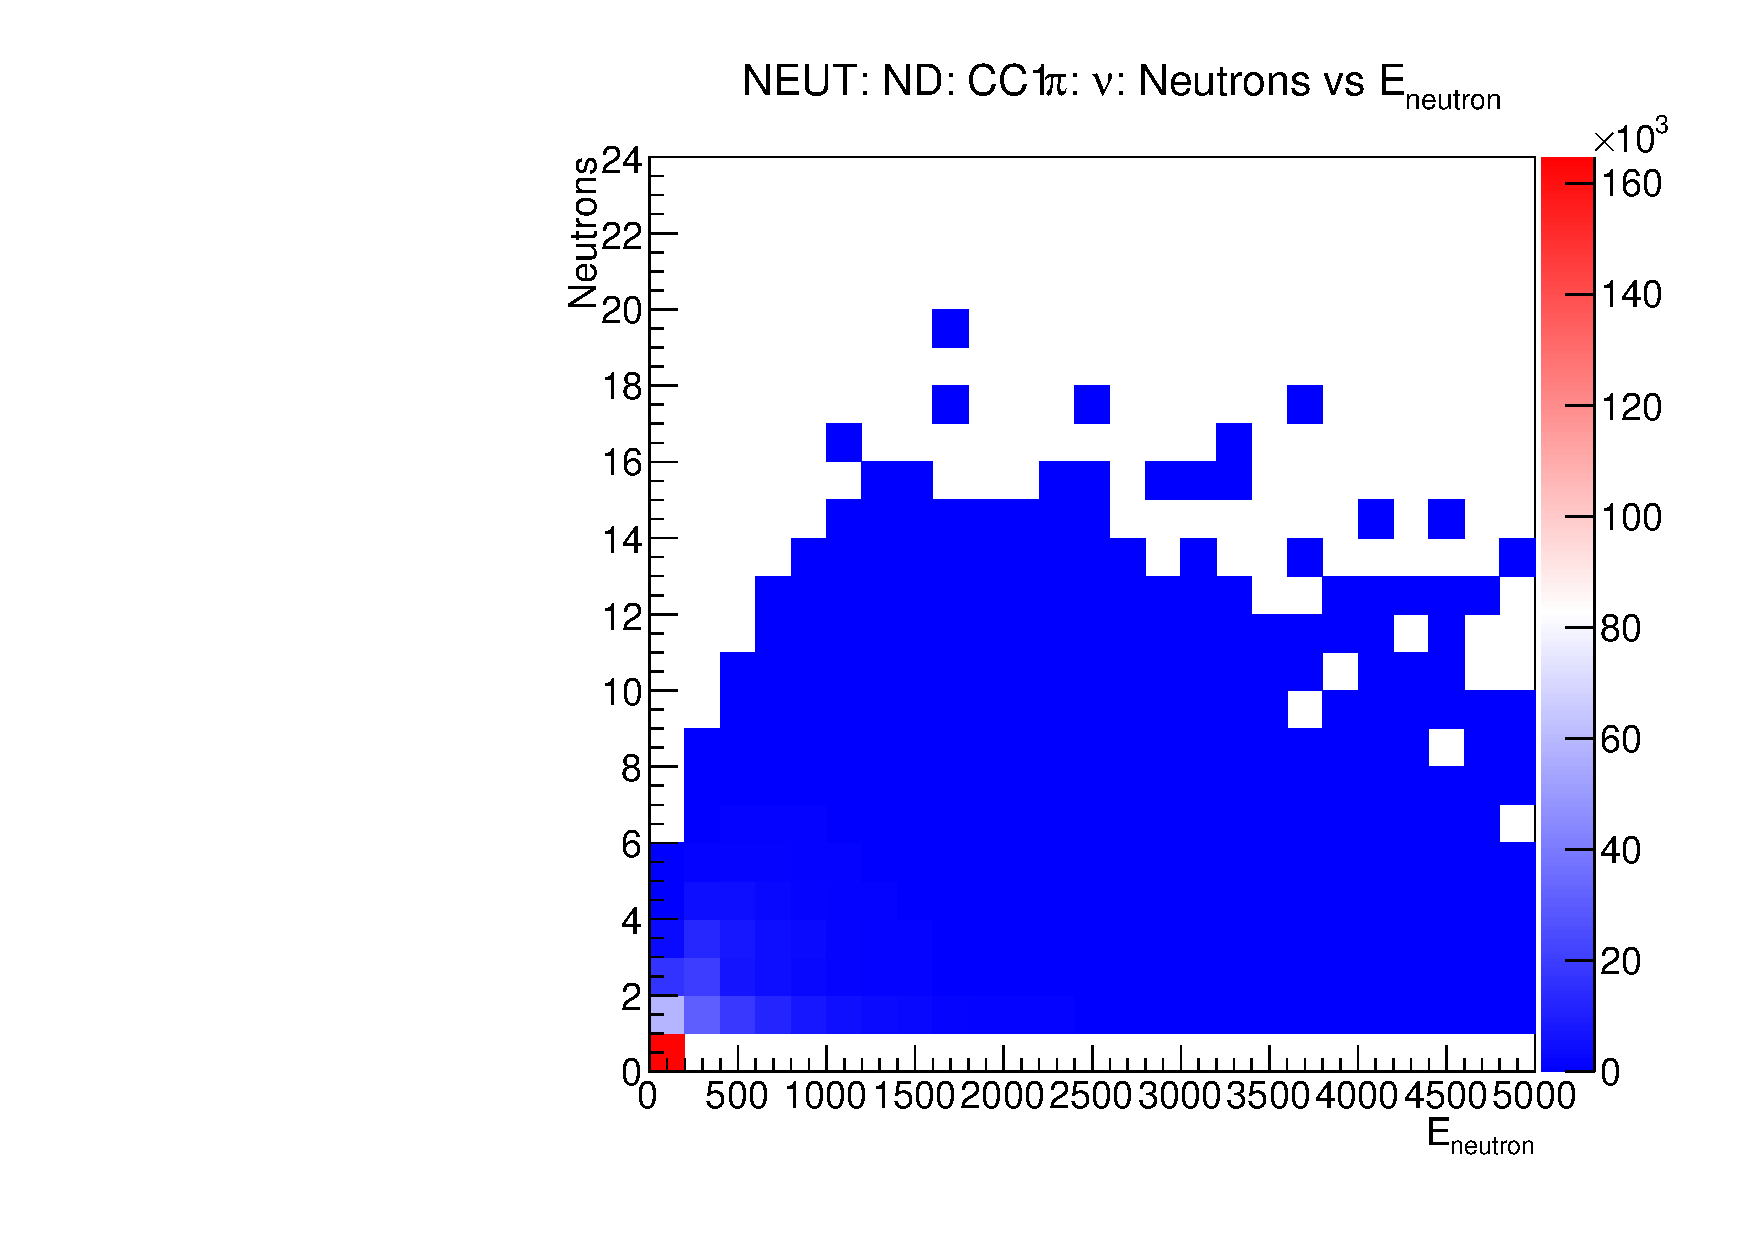
\includegraphics[width=\textwidth]{nneutrons_v_total_ene/Nneutrons_Total_ENe_res_NEUT_ND_numu.pdf}
\end{subfigure}
\begin{subfigure}[b]{0.32\textwidth}
  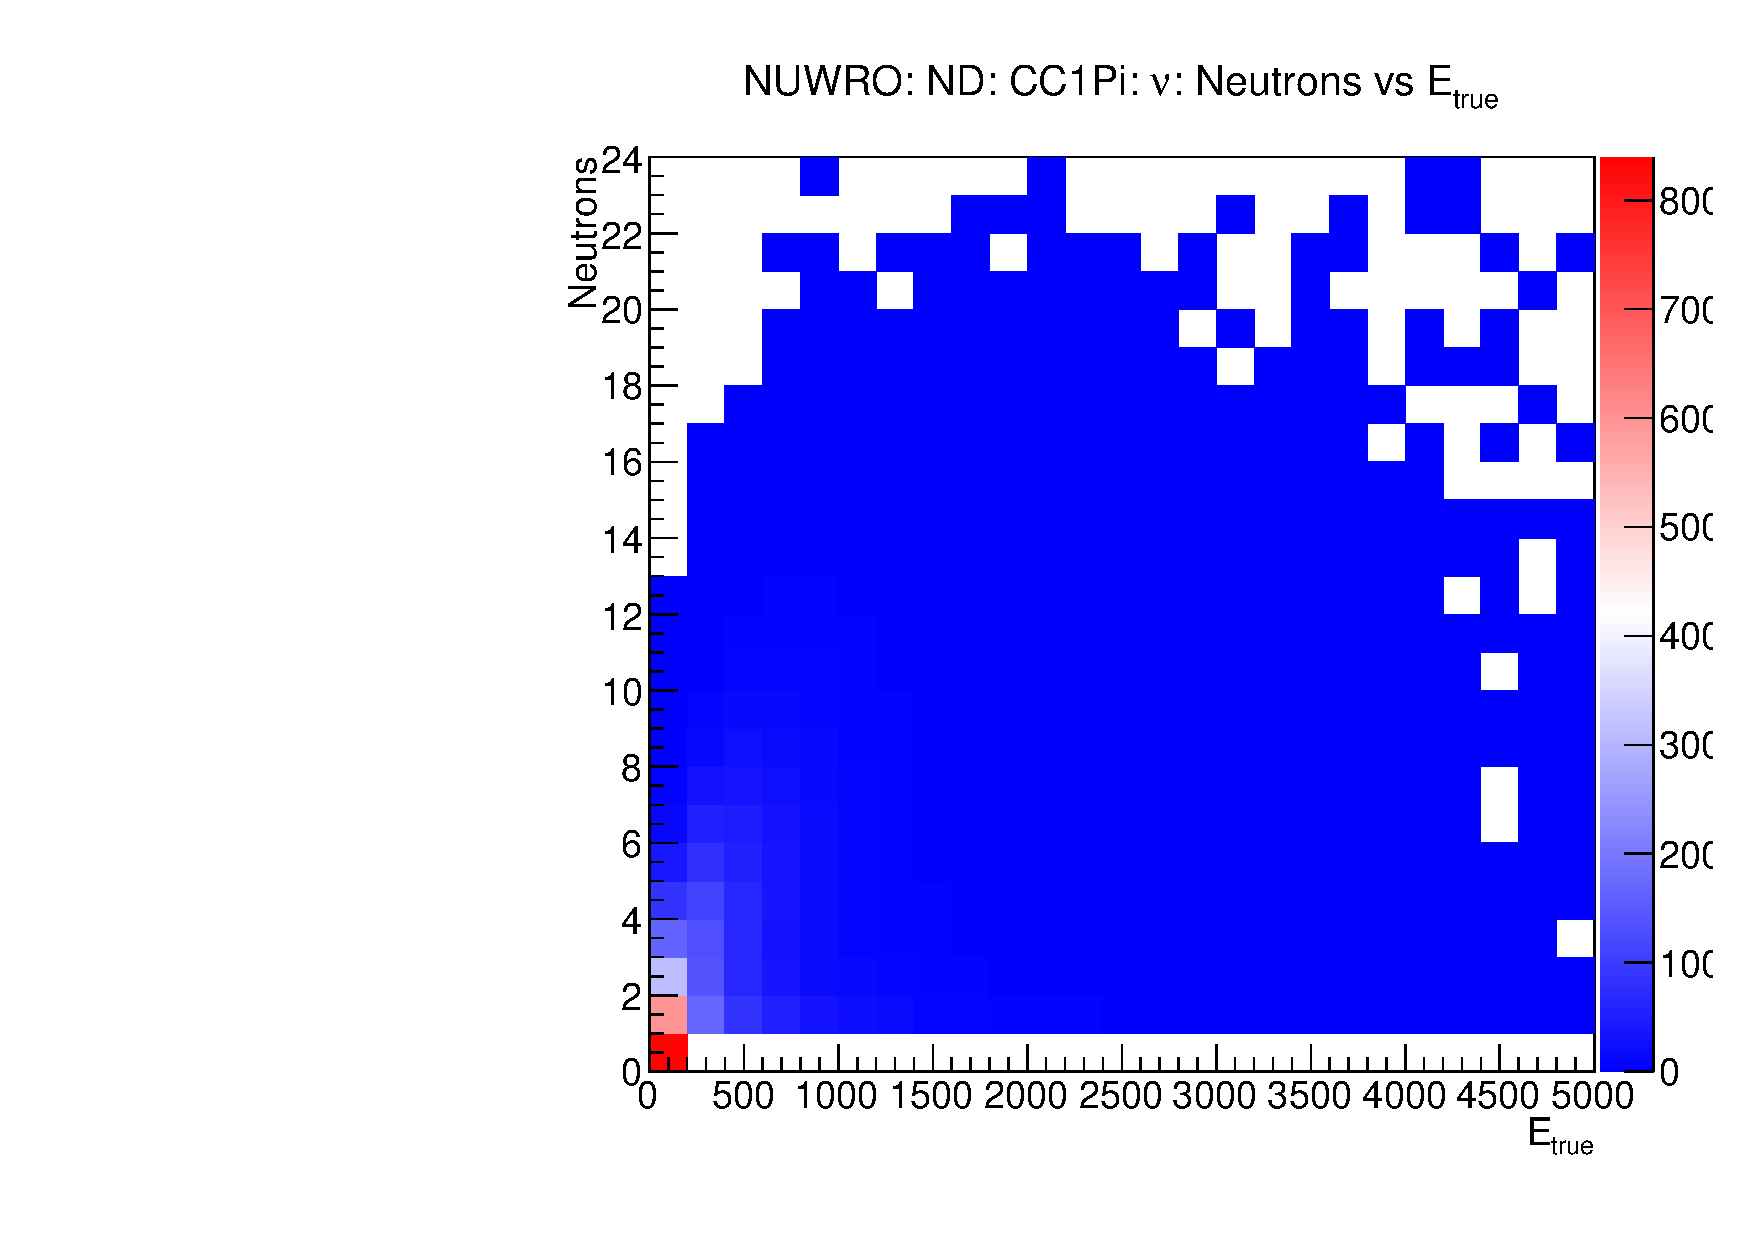
\includegraphics[width=\textwidth]{nneutrons_v_total_ene/Nneutrons_Total_ENe_res_NUWRO_ND_numu.pdf}
\end{subfigure}
\end{figure}

\begin{figure}[!htb]
\centering
\begin{subfigure}[b]{0.32\textwidth}
  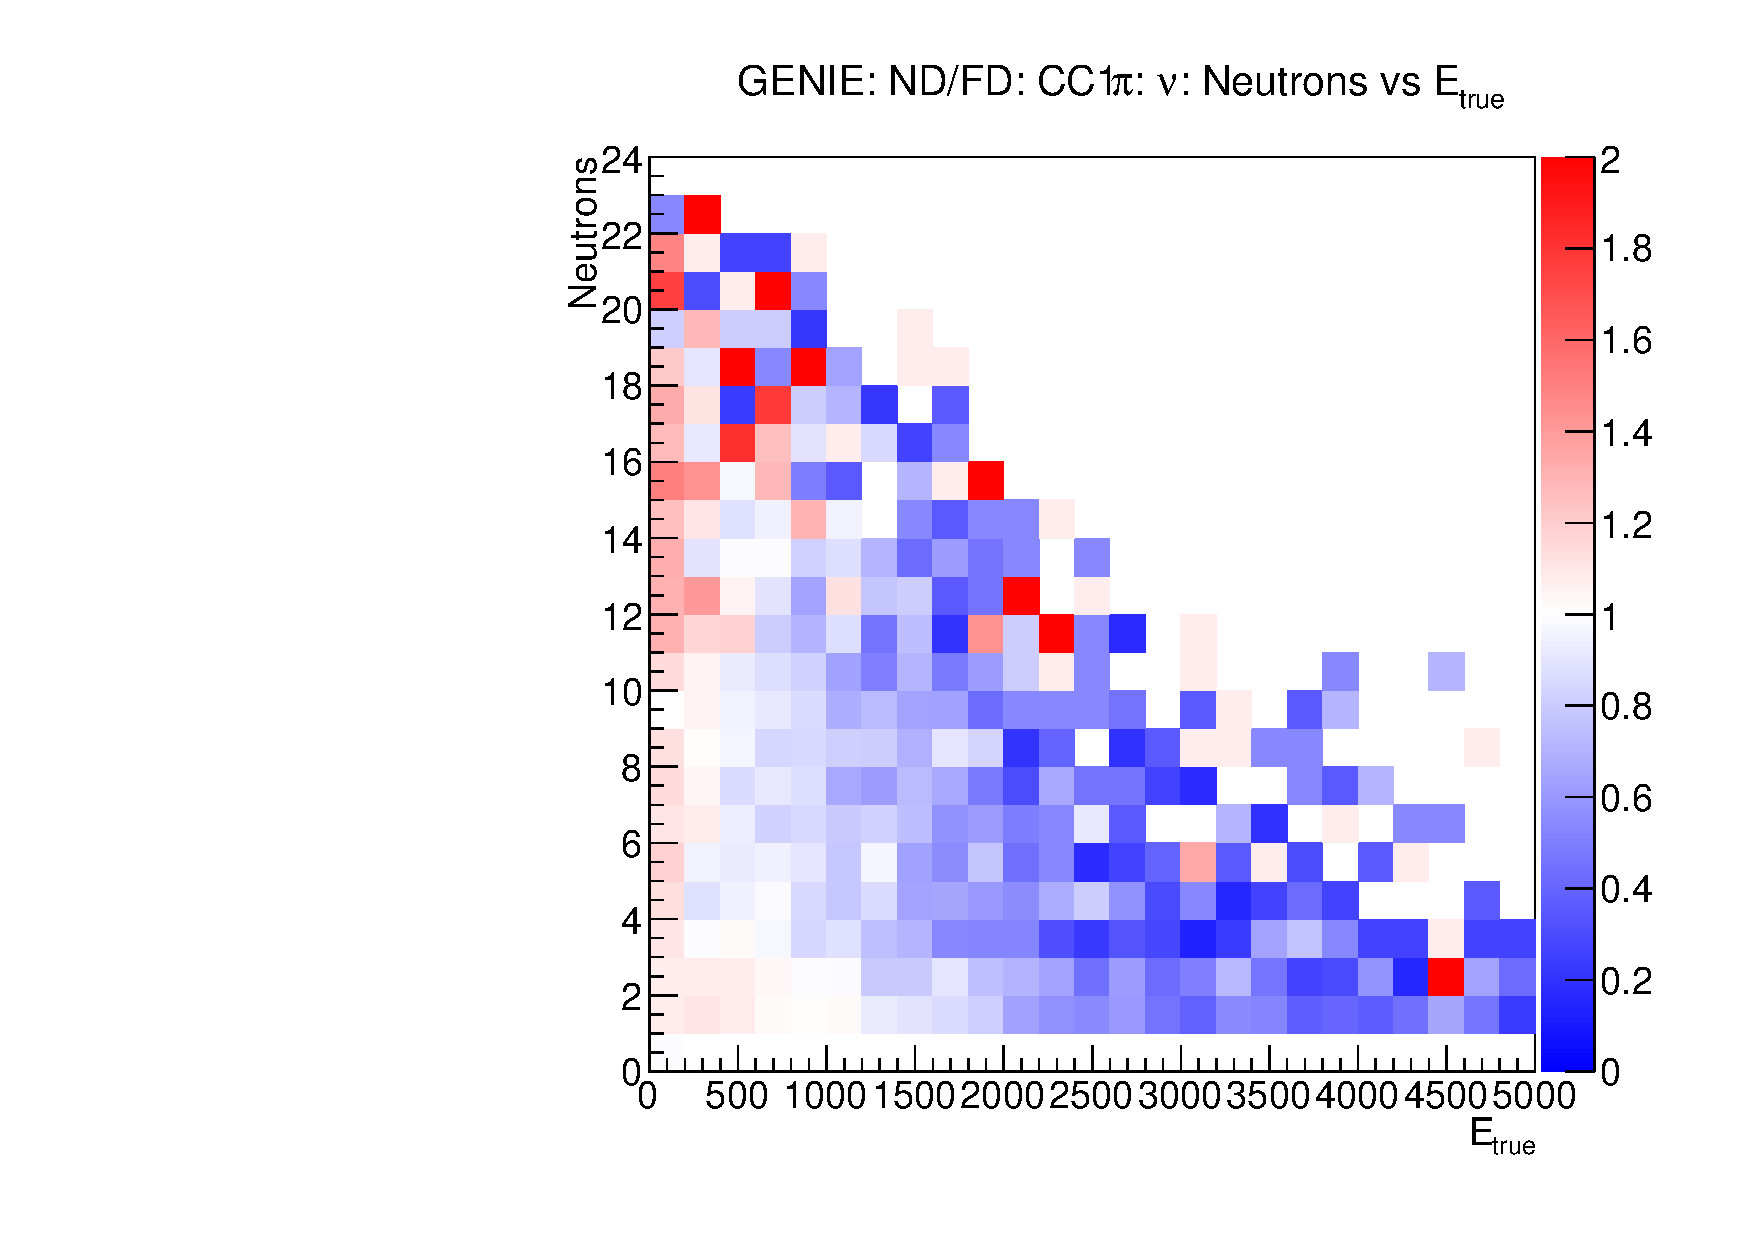
\includegraphics[width=\textwidth]{nneutrons_v_total_ene/Nneutrons_Total_ENe_res_GENIE_ND_FD_numu_norm.pdf}
\end{subfigure}
\begin{subfigure}[b]{0.32\textwidth}
  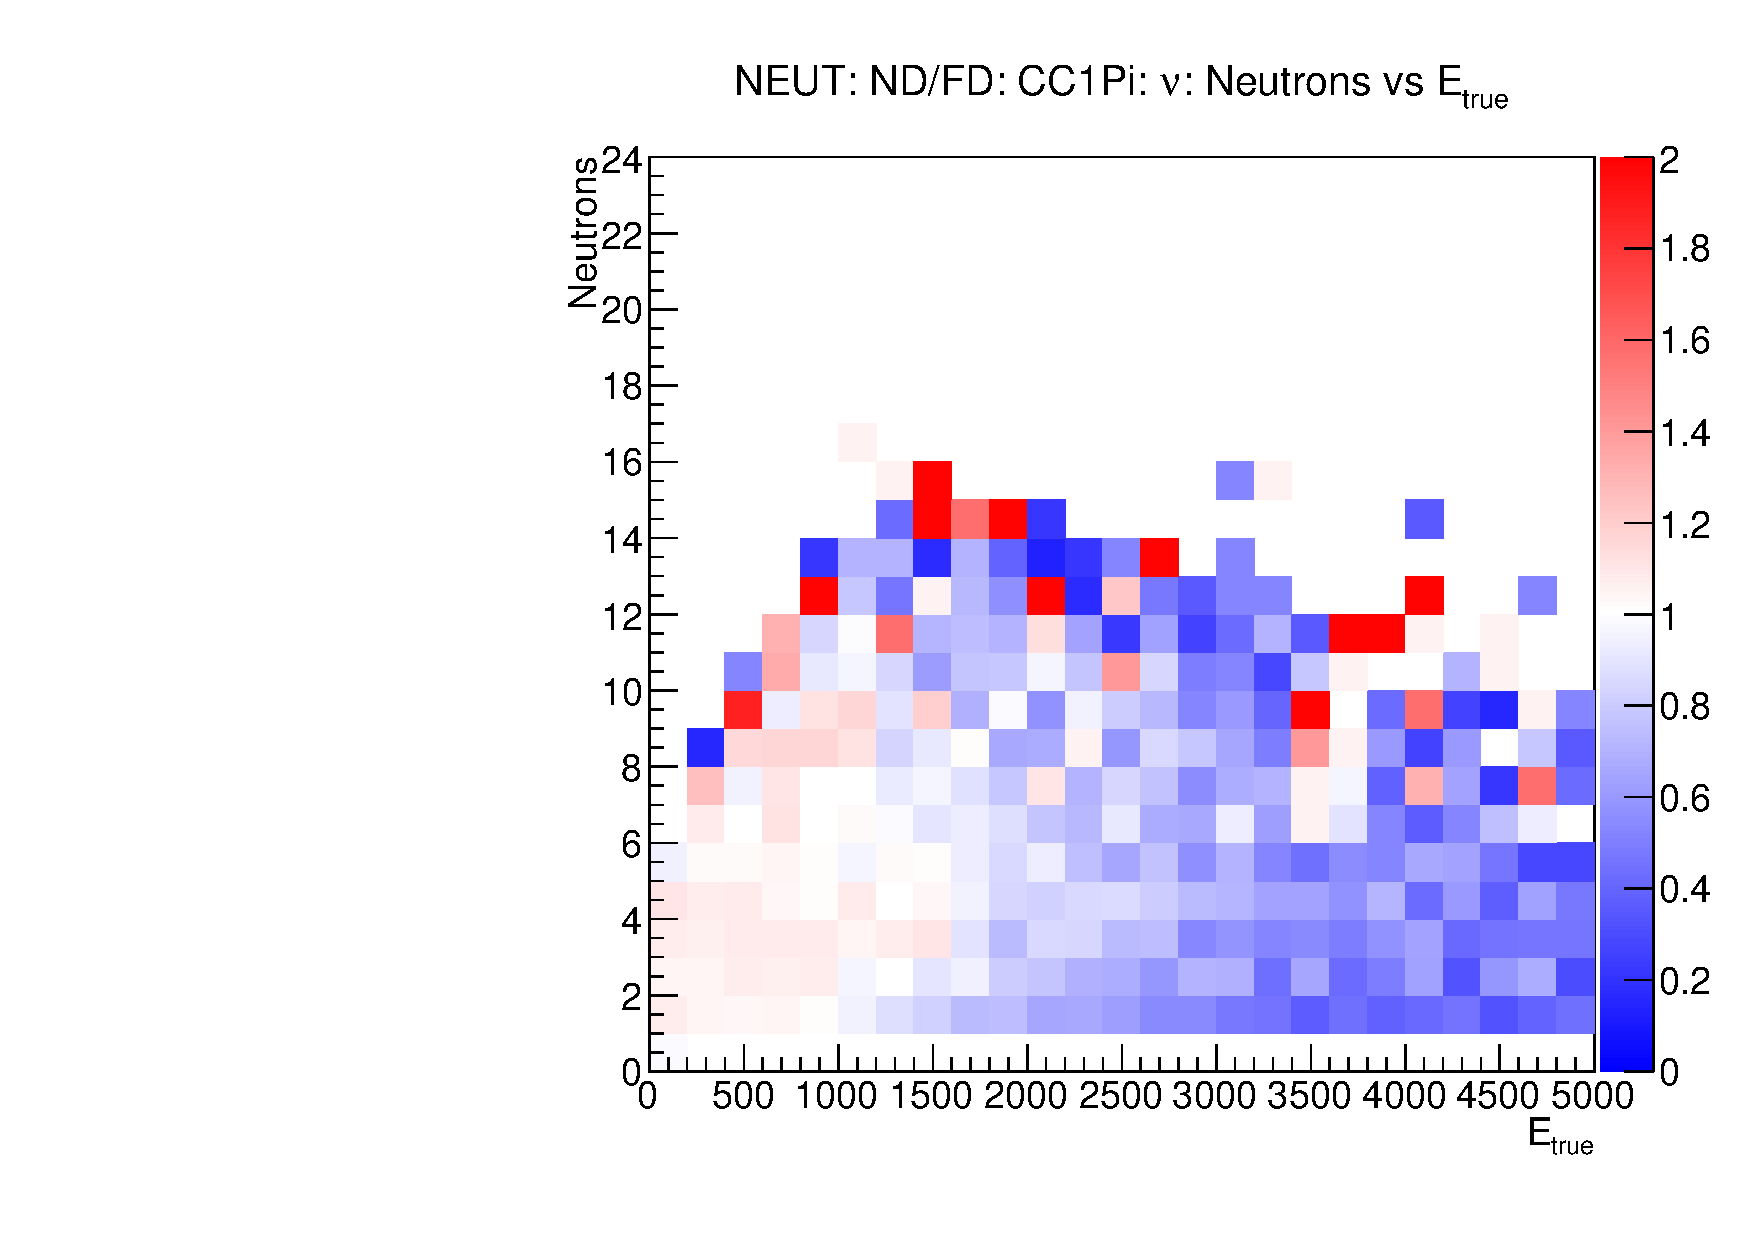
\includegraphics[width=\textwidth]{nneutrons_v_total_ene/Nneutrons_Total_ENe_res_NEUT_ND_FD_numu_norm.pdf}
\end{subfigure}
\begin{subfigure}[b]{0.32\textwidth}
  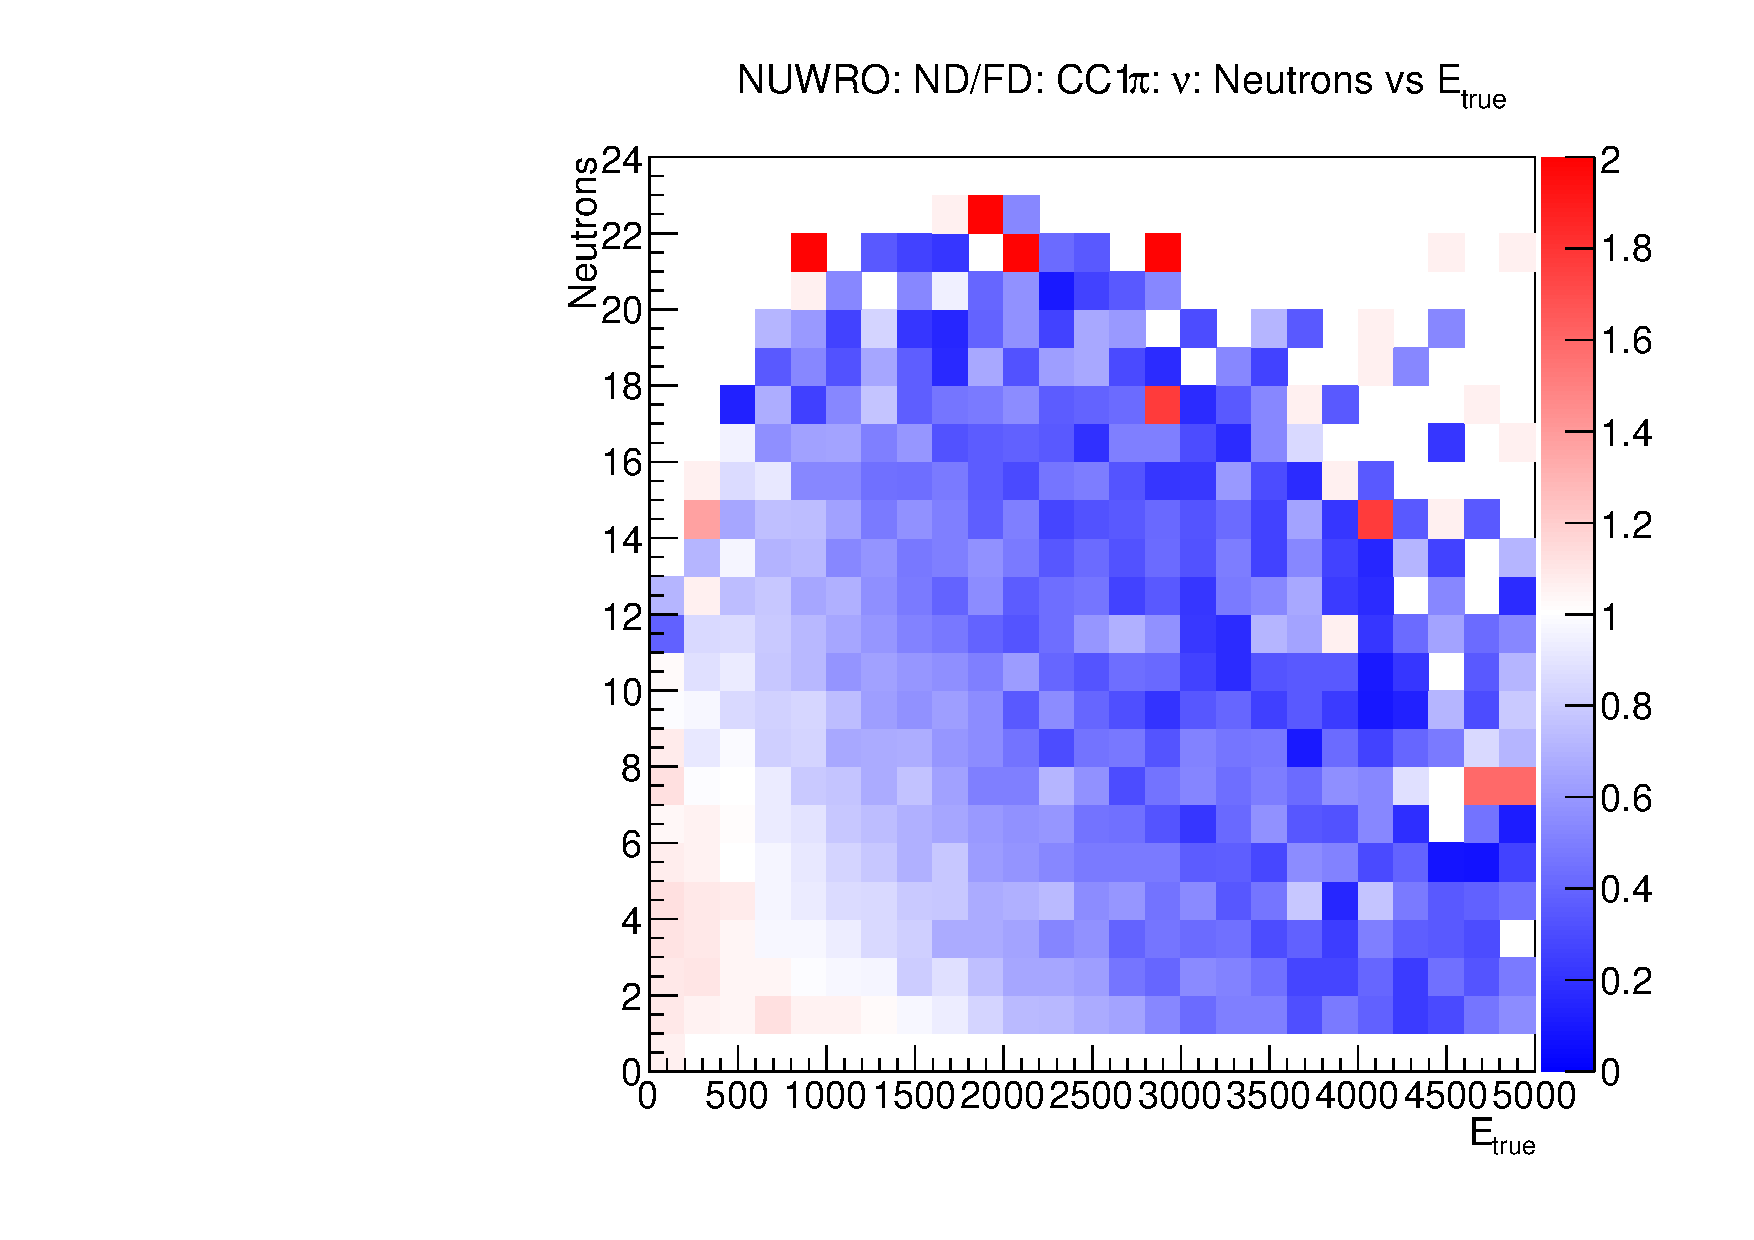
\includegraphics[width=\textwidth]{nneutrons_v_total_ene/Nneutrons_Total_ENe_res_NUWRO_ND_FD_numu_norm.pdf}
\end{subfigure}
\end{figure}

\begin{figure}[!htb]
\centering
\begin{subfigure}[b]{0.32\textwidth}
  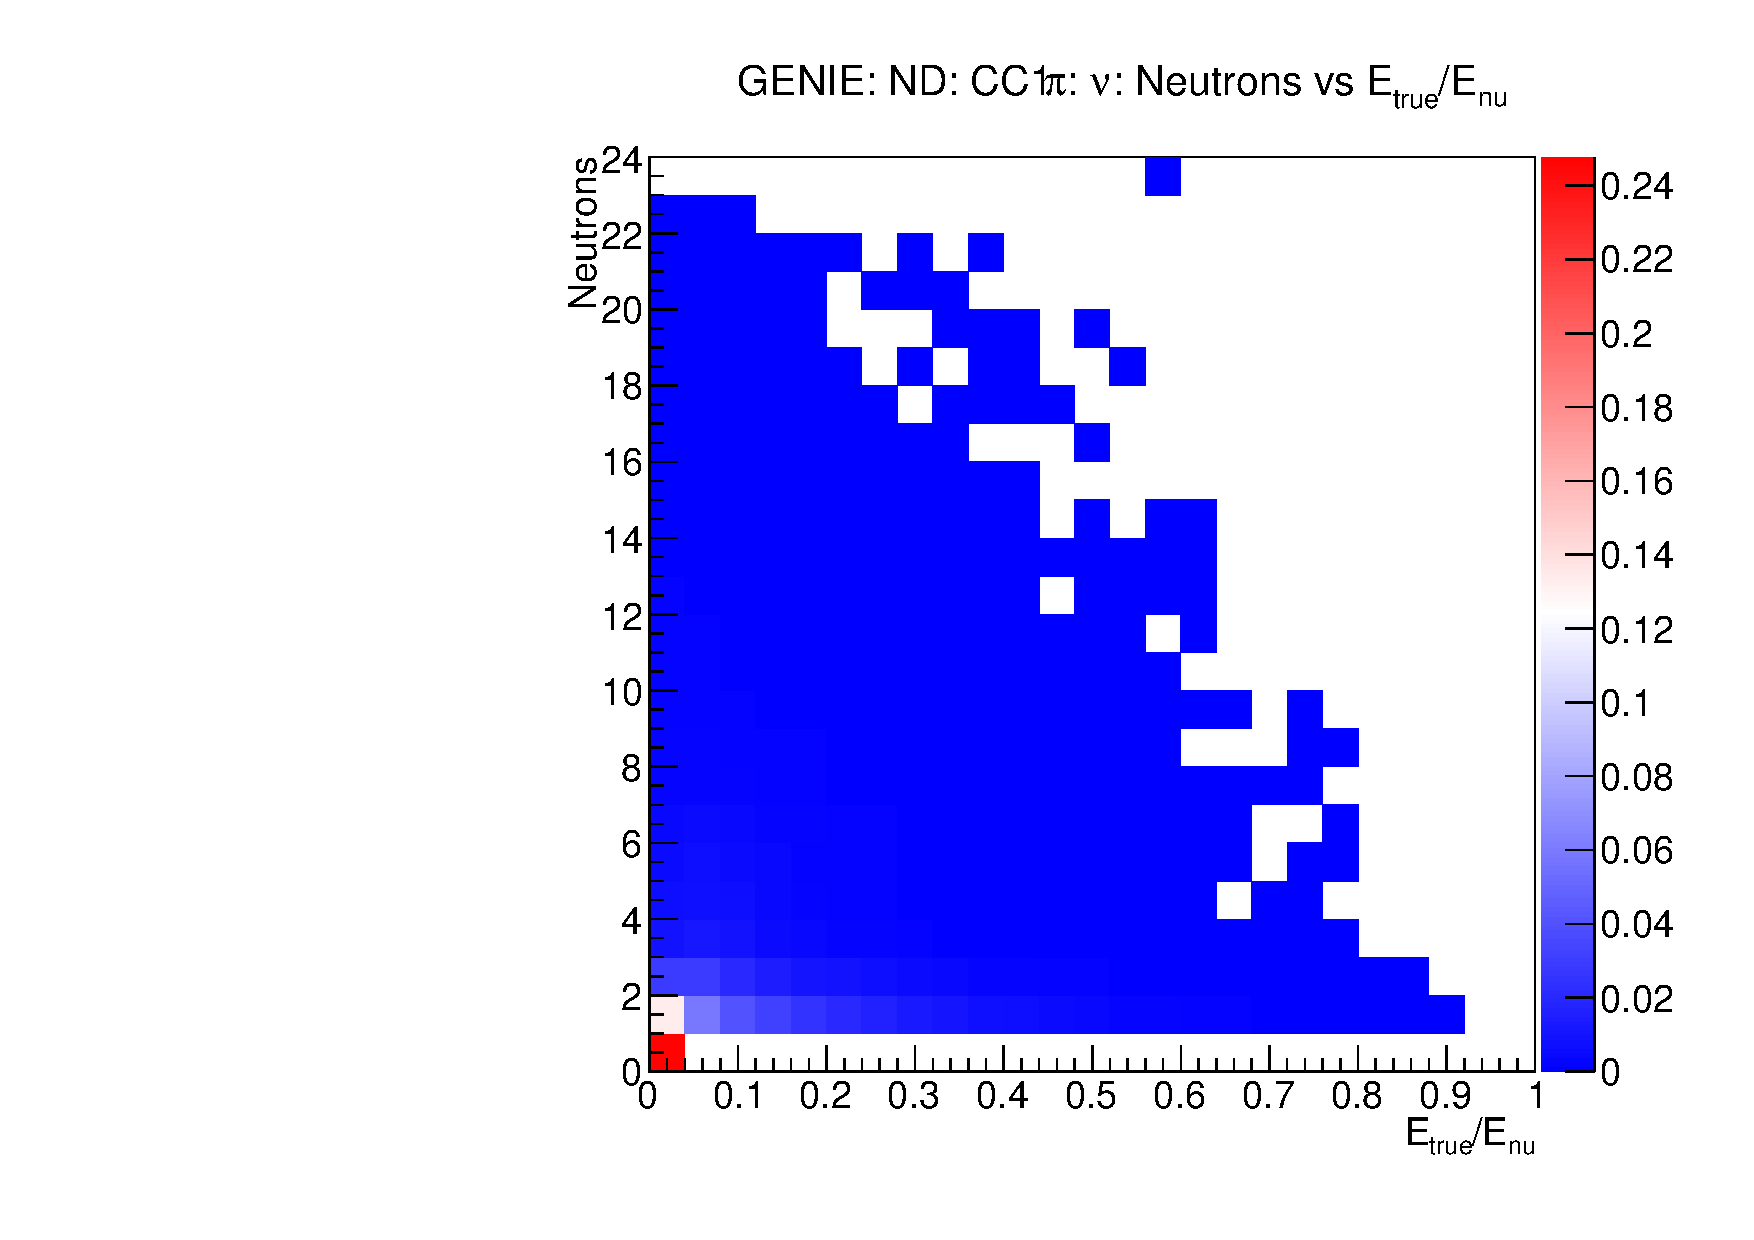
\includegraphics[width=\textwidth]{nneutrons_ene_enu/Nneutrons_Enu_true_res_GENIE_ND_numu_norm.pdf}
\end{subfigure}
\begin{subfigure}[b]{0.32\textwidth}
  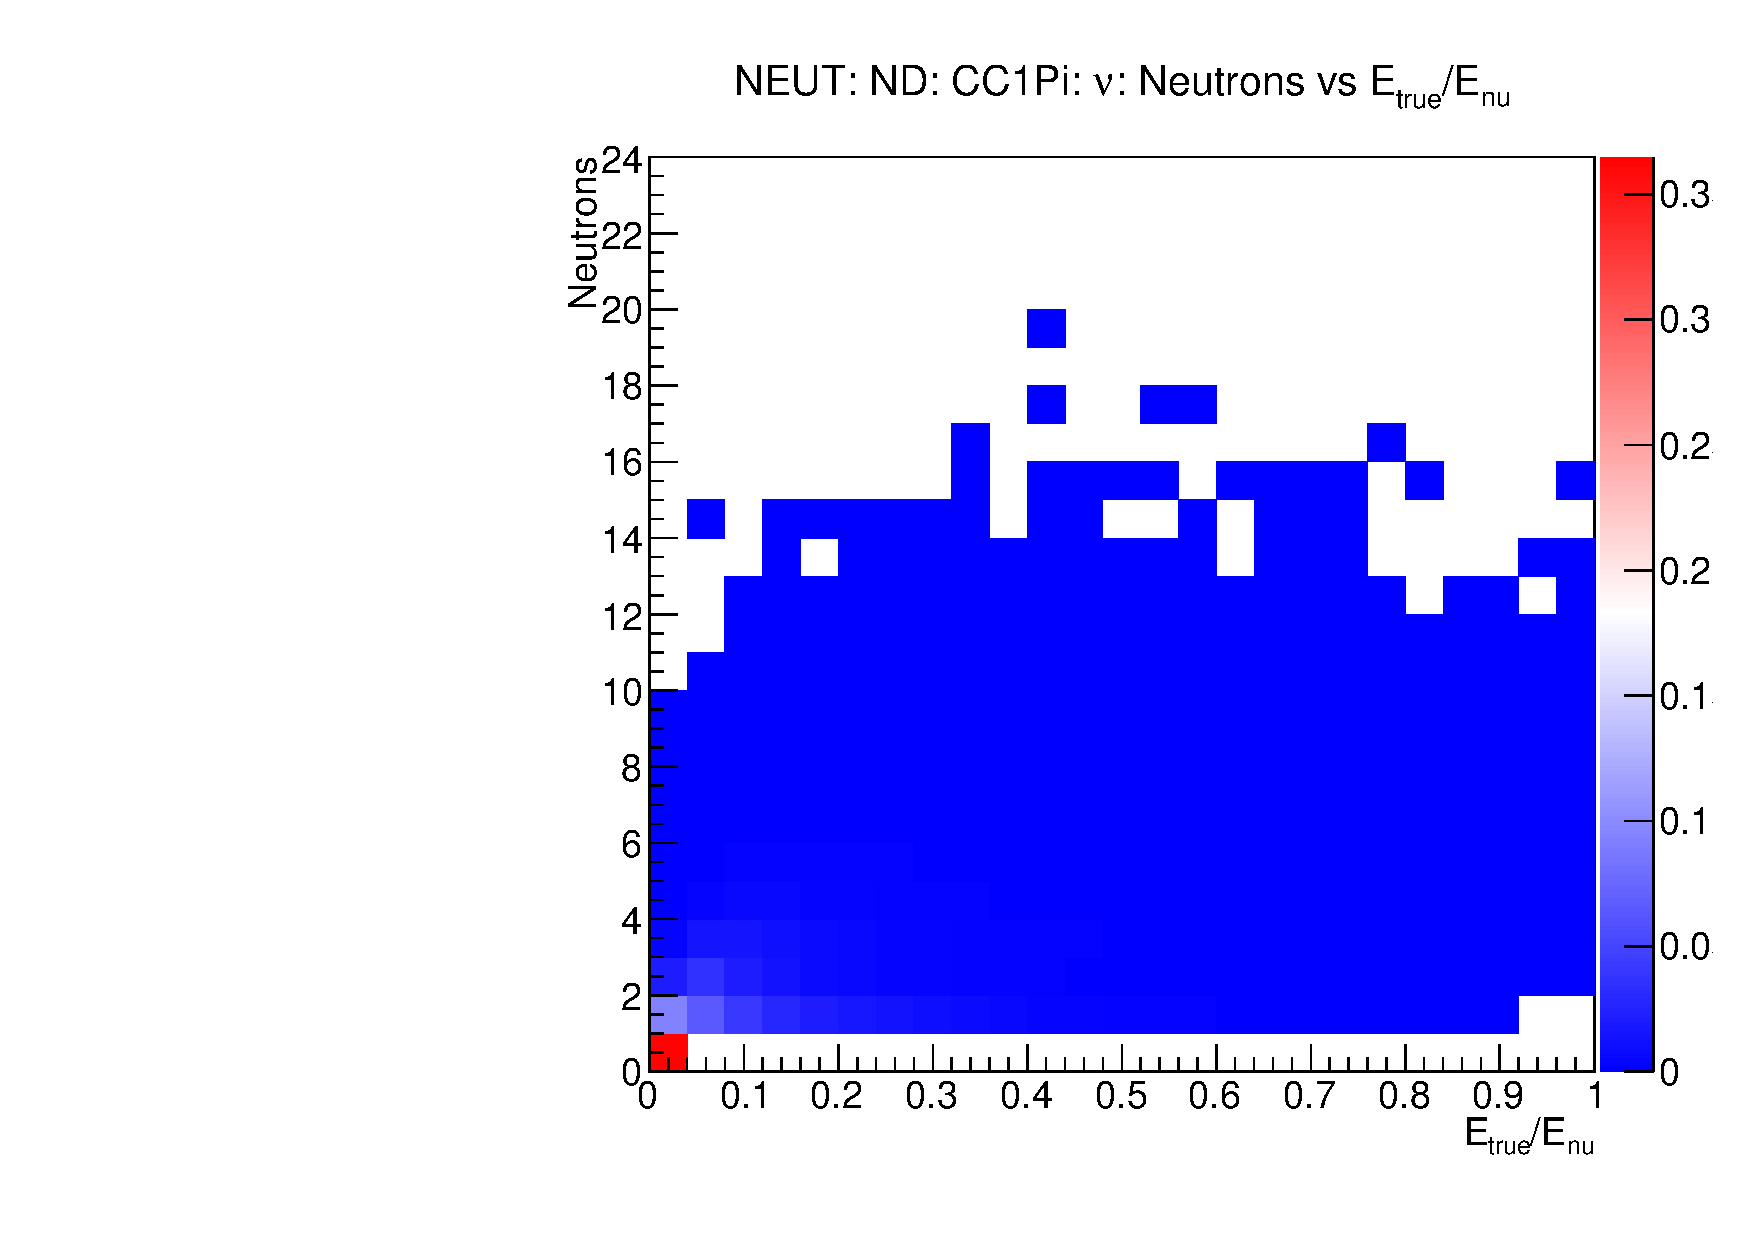
\includegraphics[width=\textwidth]{nneutrons_ene_enu/Nneutrons_Enu_true_res_NEUT_ND_numu_norm.pdf}
\end{subfigure}
\begin{subfigure}[b]{0.32\textwidth}
  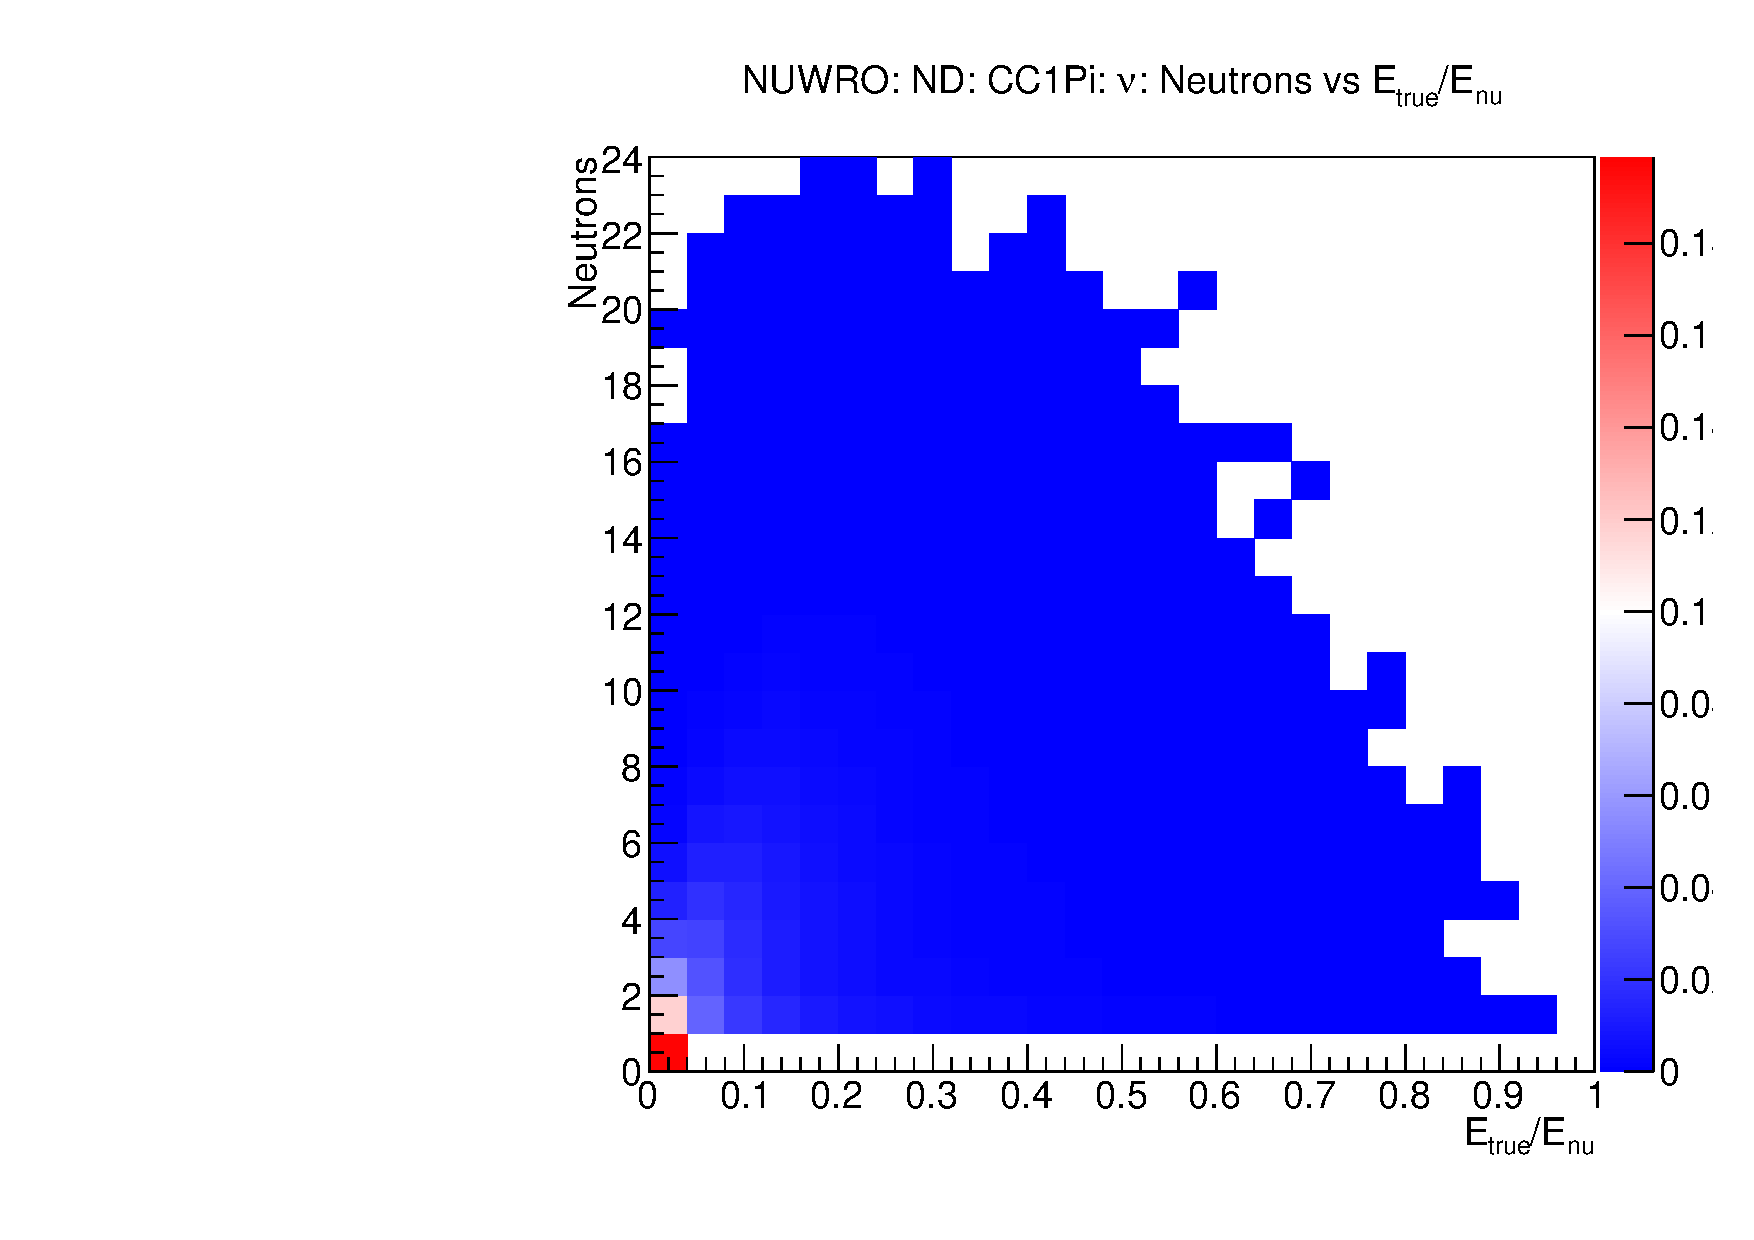
\includegraphics[width=\textwidth]{nneutrons_ene_enu/Nneutrons_Enu_true_res_NUWRO_ND_numu_norm.pdf}
\end{subfigure}
\end{figure}
\FloatBarrier

\subsubsection{CC-Other}

\begin{figure}[!htb]
\centering
\begin{subfigure}[b]{0.32\textwidth}
  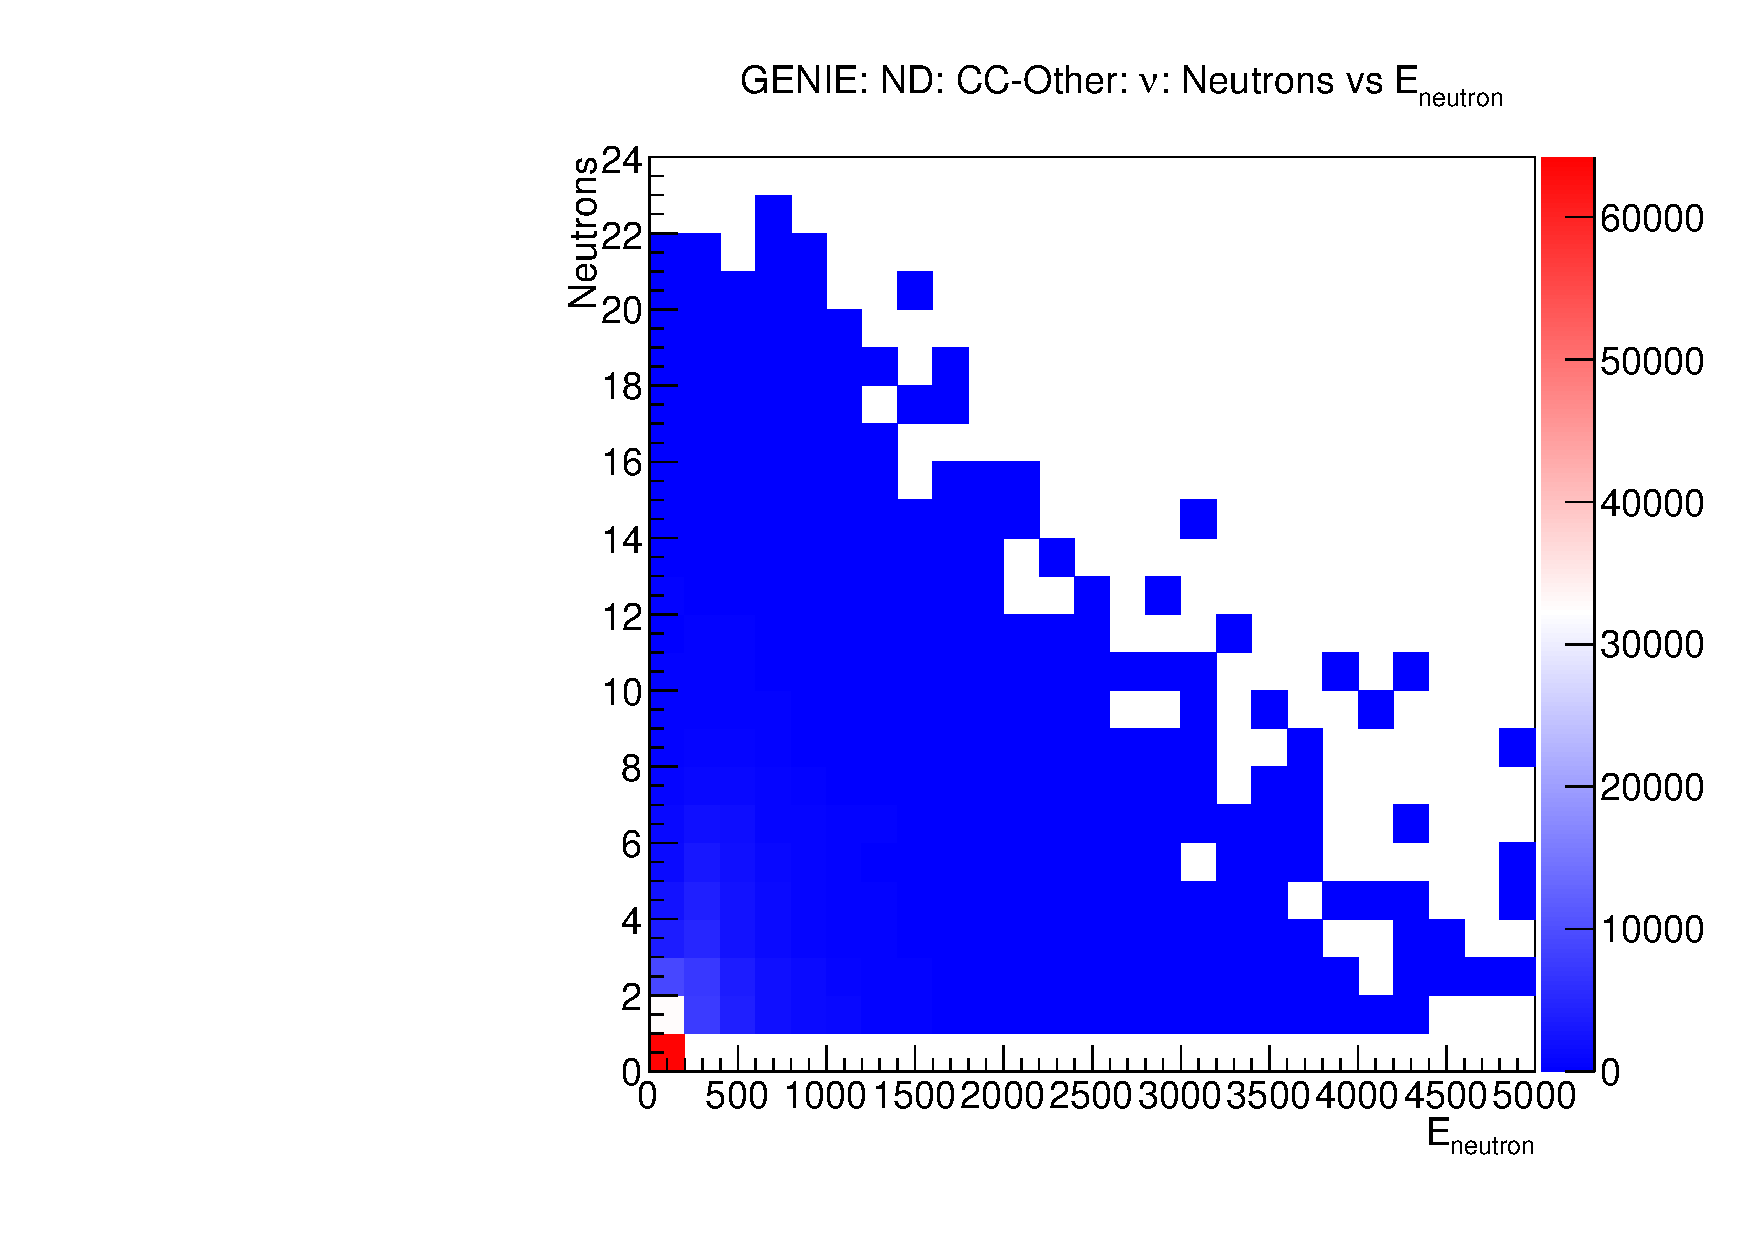
\includegraphics[width=\textwidth]{nneutrons_v_total_ene/Nneutrons_Total_ENe_dis_GENIE_ND_numu.pdf}
\end{subfigure}
\begin{subfigure}[b]{0.32\textwidth}
  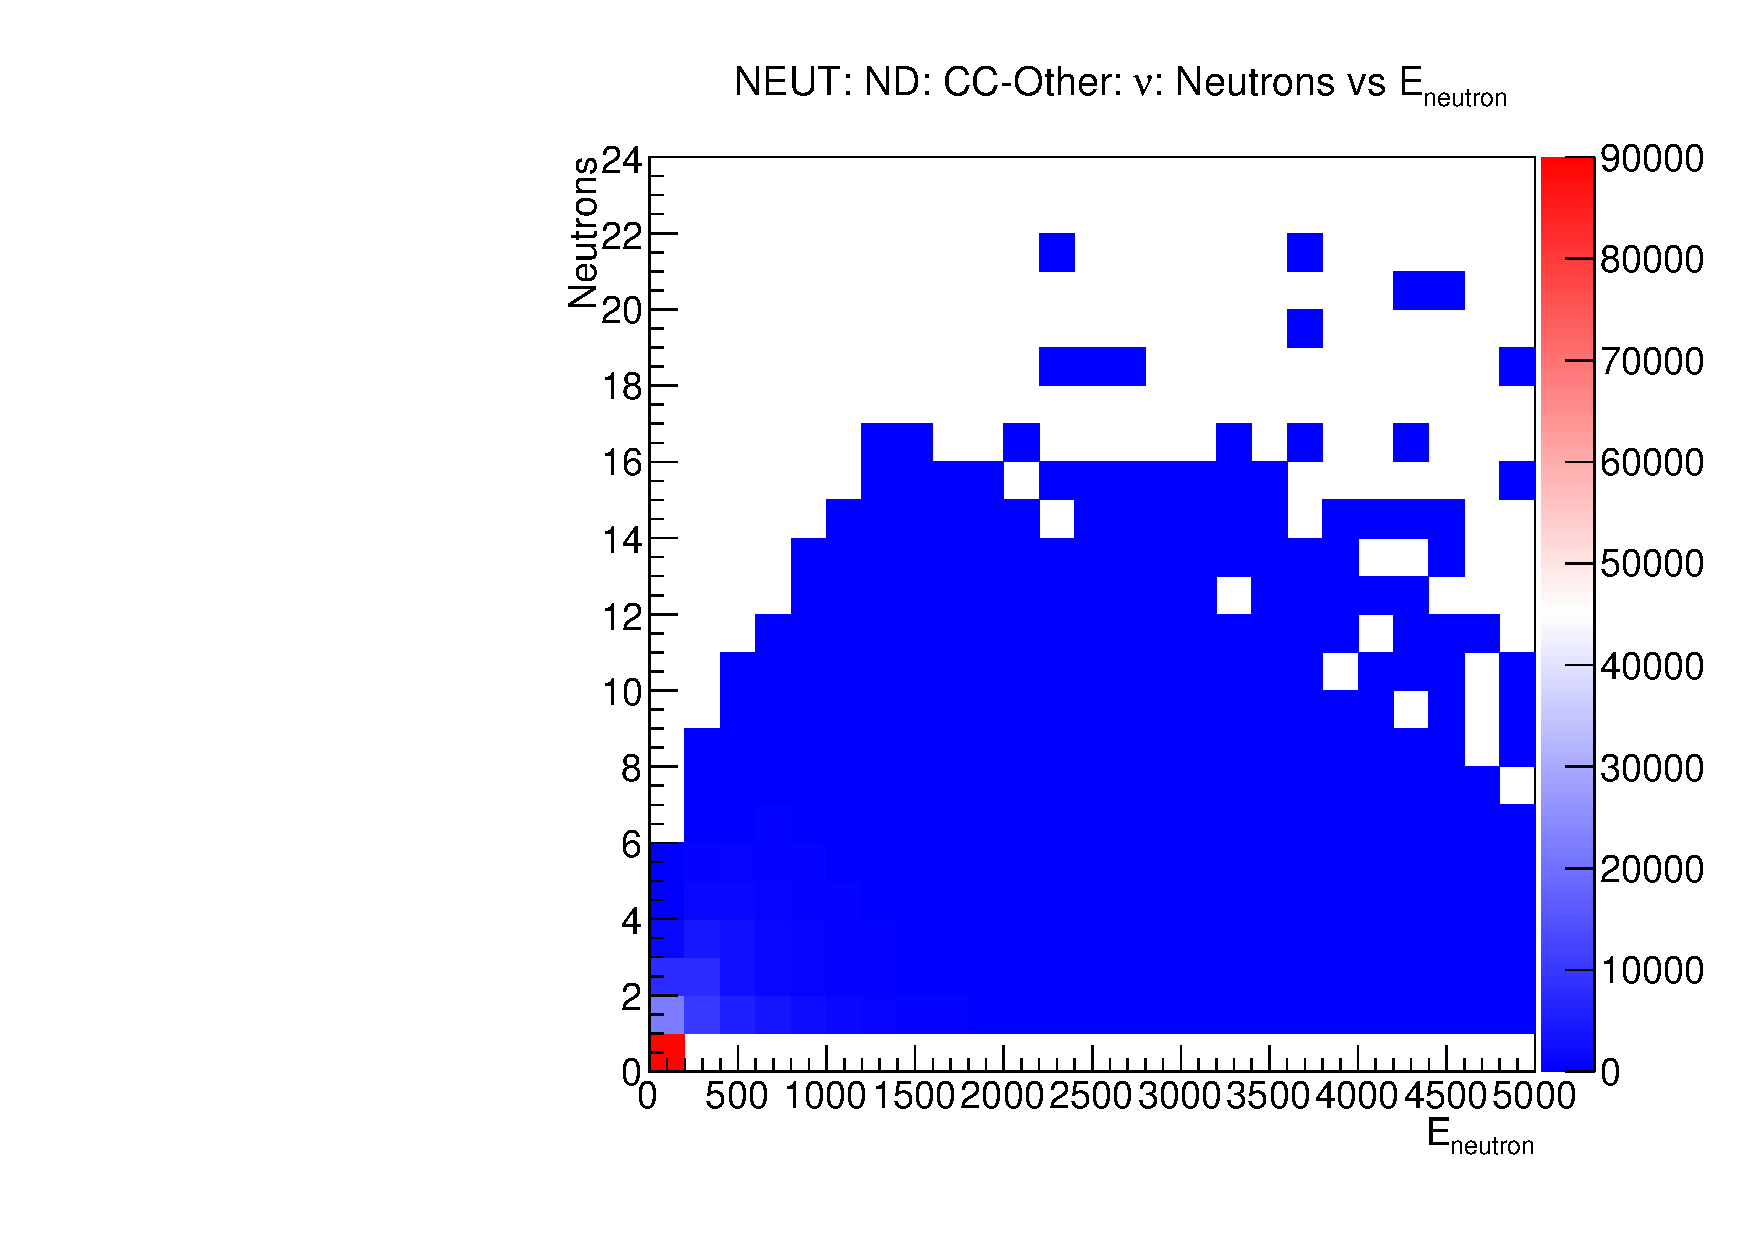
\includegraphics[width=\textwidth]{nneutrons_v_total_ene/Nneutrons_Total_ENe_dis_NEUT_ND_numu.pdf}
\end{subfigure}
\begin{subfigure}[b]{0.32\textwidth}
  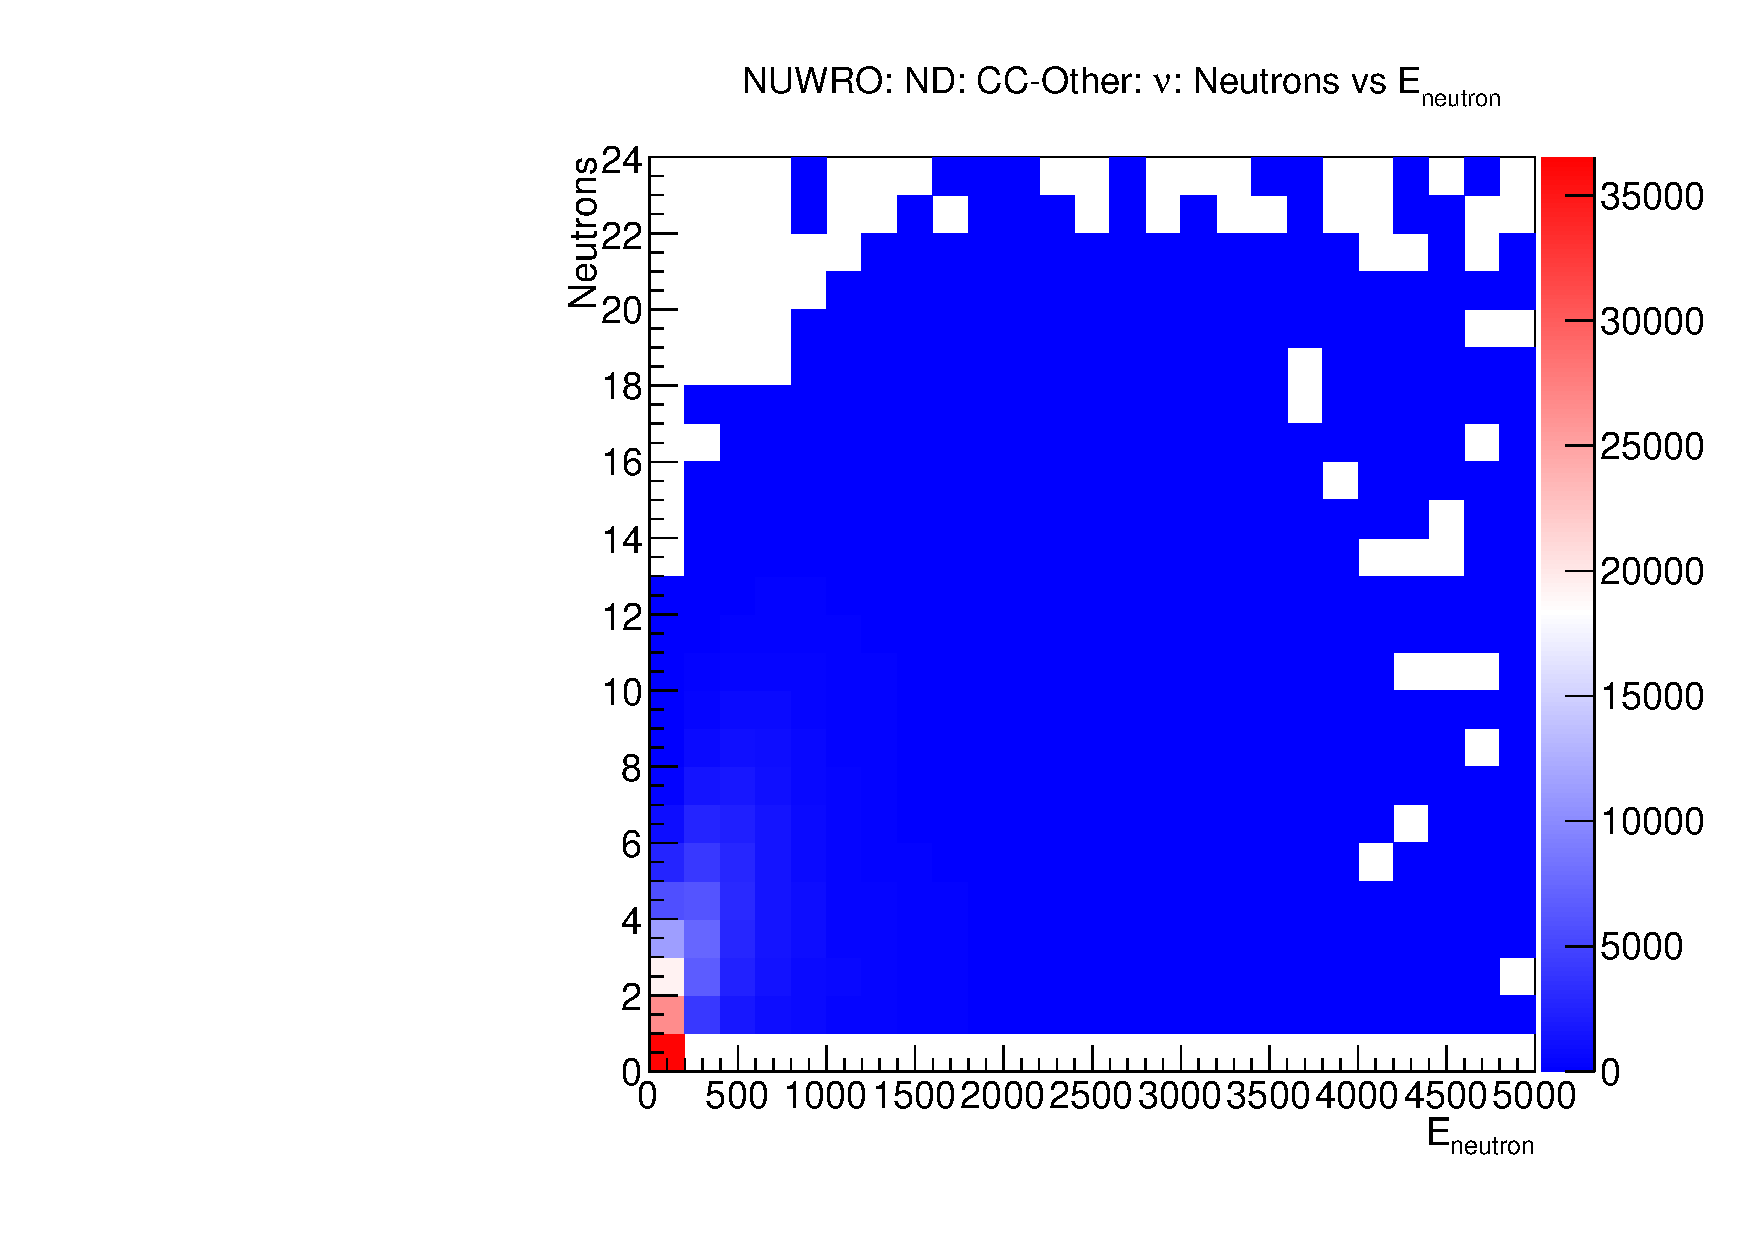
\includegraphics[width=\textwidth]{nneutrons_v_total_ene/Nneutrons_Total_ENe_dis_NUWRO_ND_numu.pdf}
\end{subfigure}
\end{figure}

\begin{figure}[!htb]
\centering
\begin{subfigure}[b]{0.32\textwidth}
  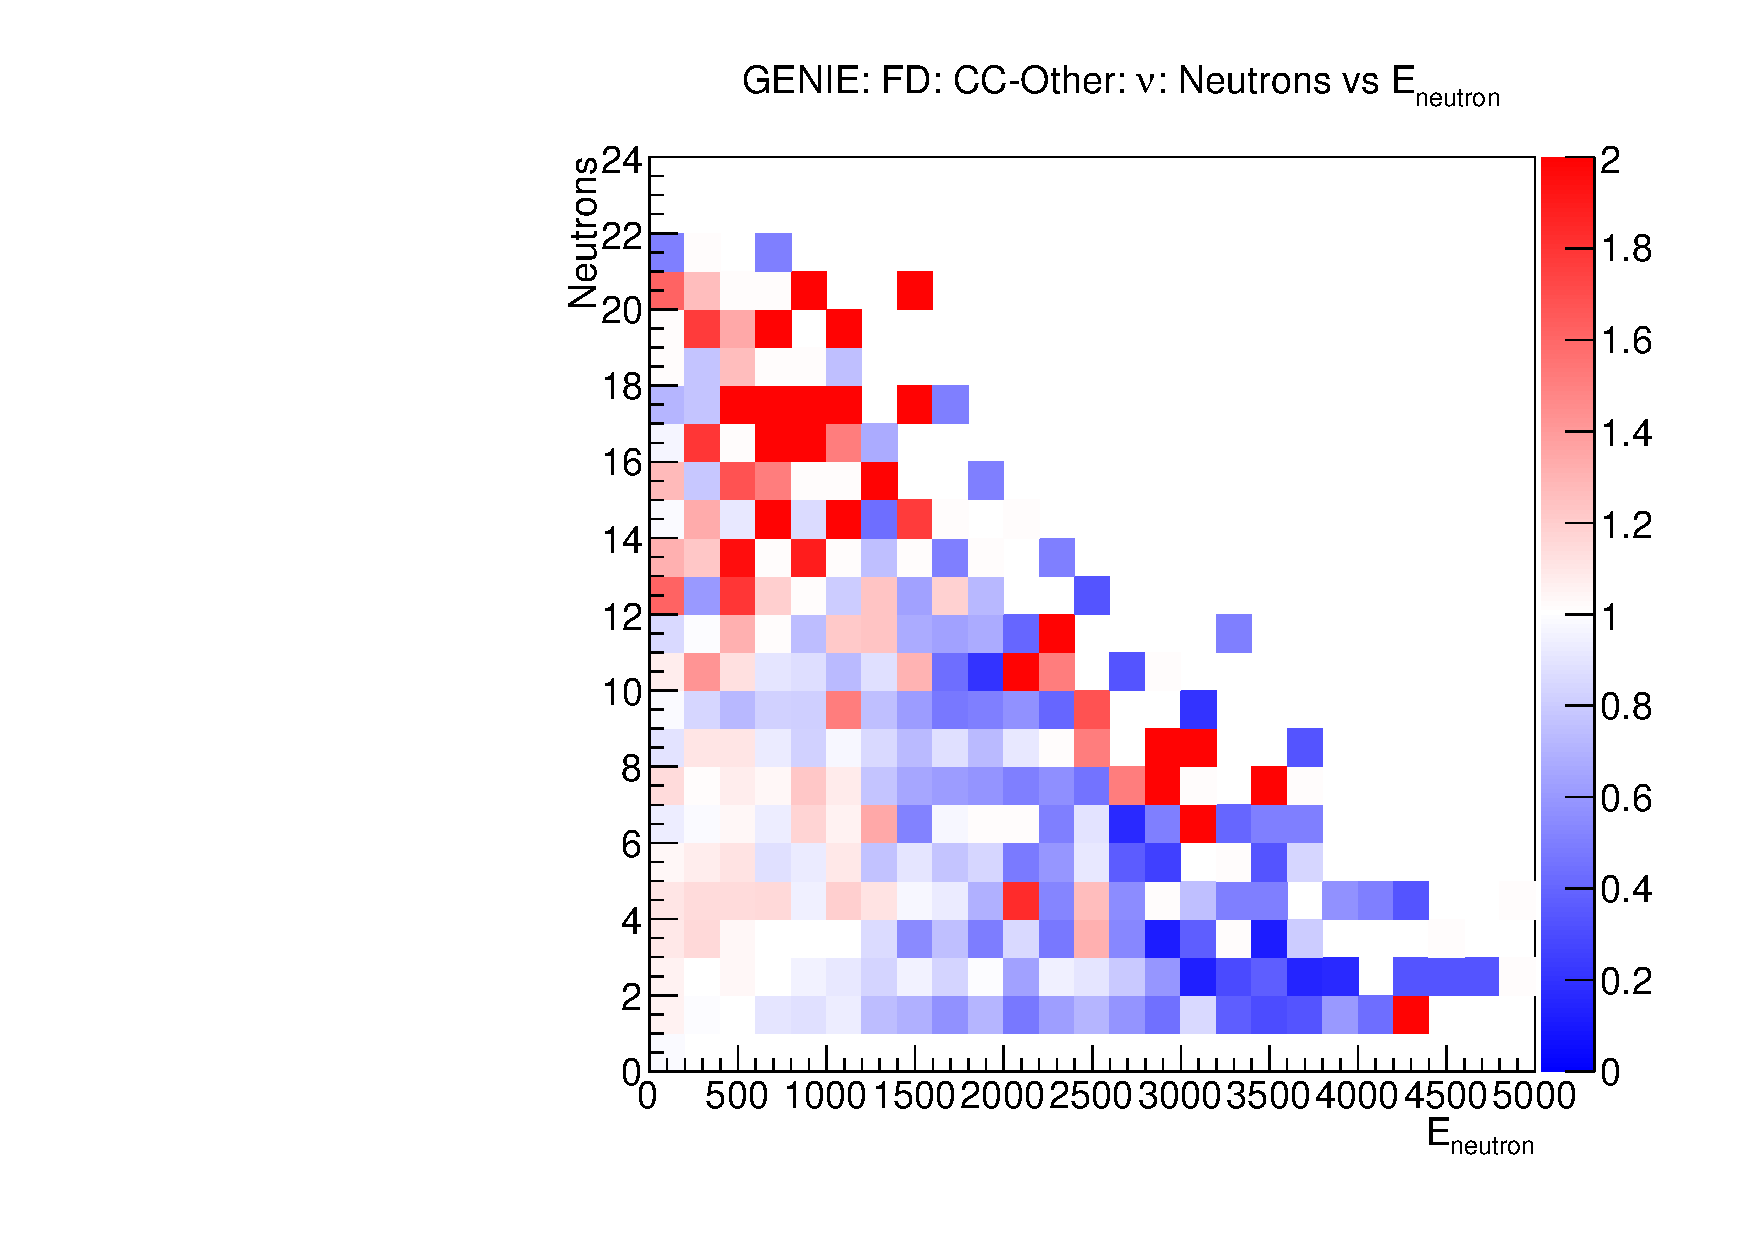
\includegraphics[width=\textwidth]{nneutrons_v_total_ene/Nneutrons_Total_ENe_dis_GENIE_ND_FD_numu_norm.pdf}
\end{subfigure}
\begin{subfigure}[b]{0.32\textwidth}
  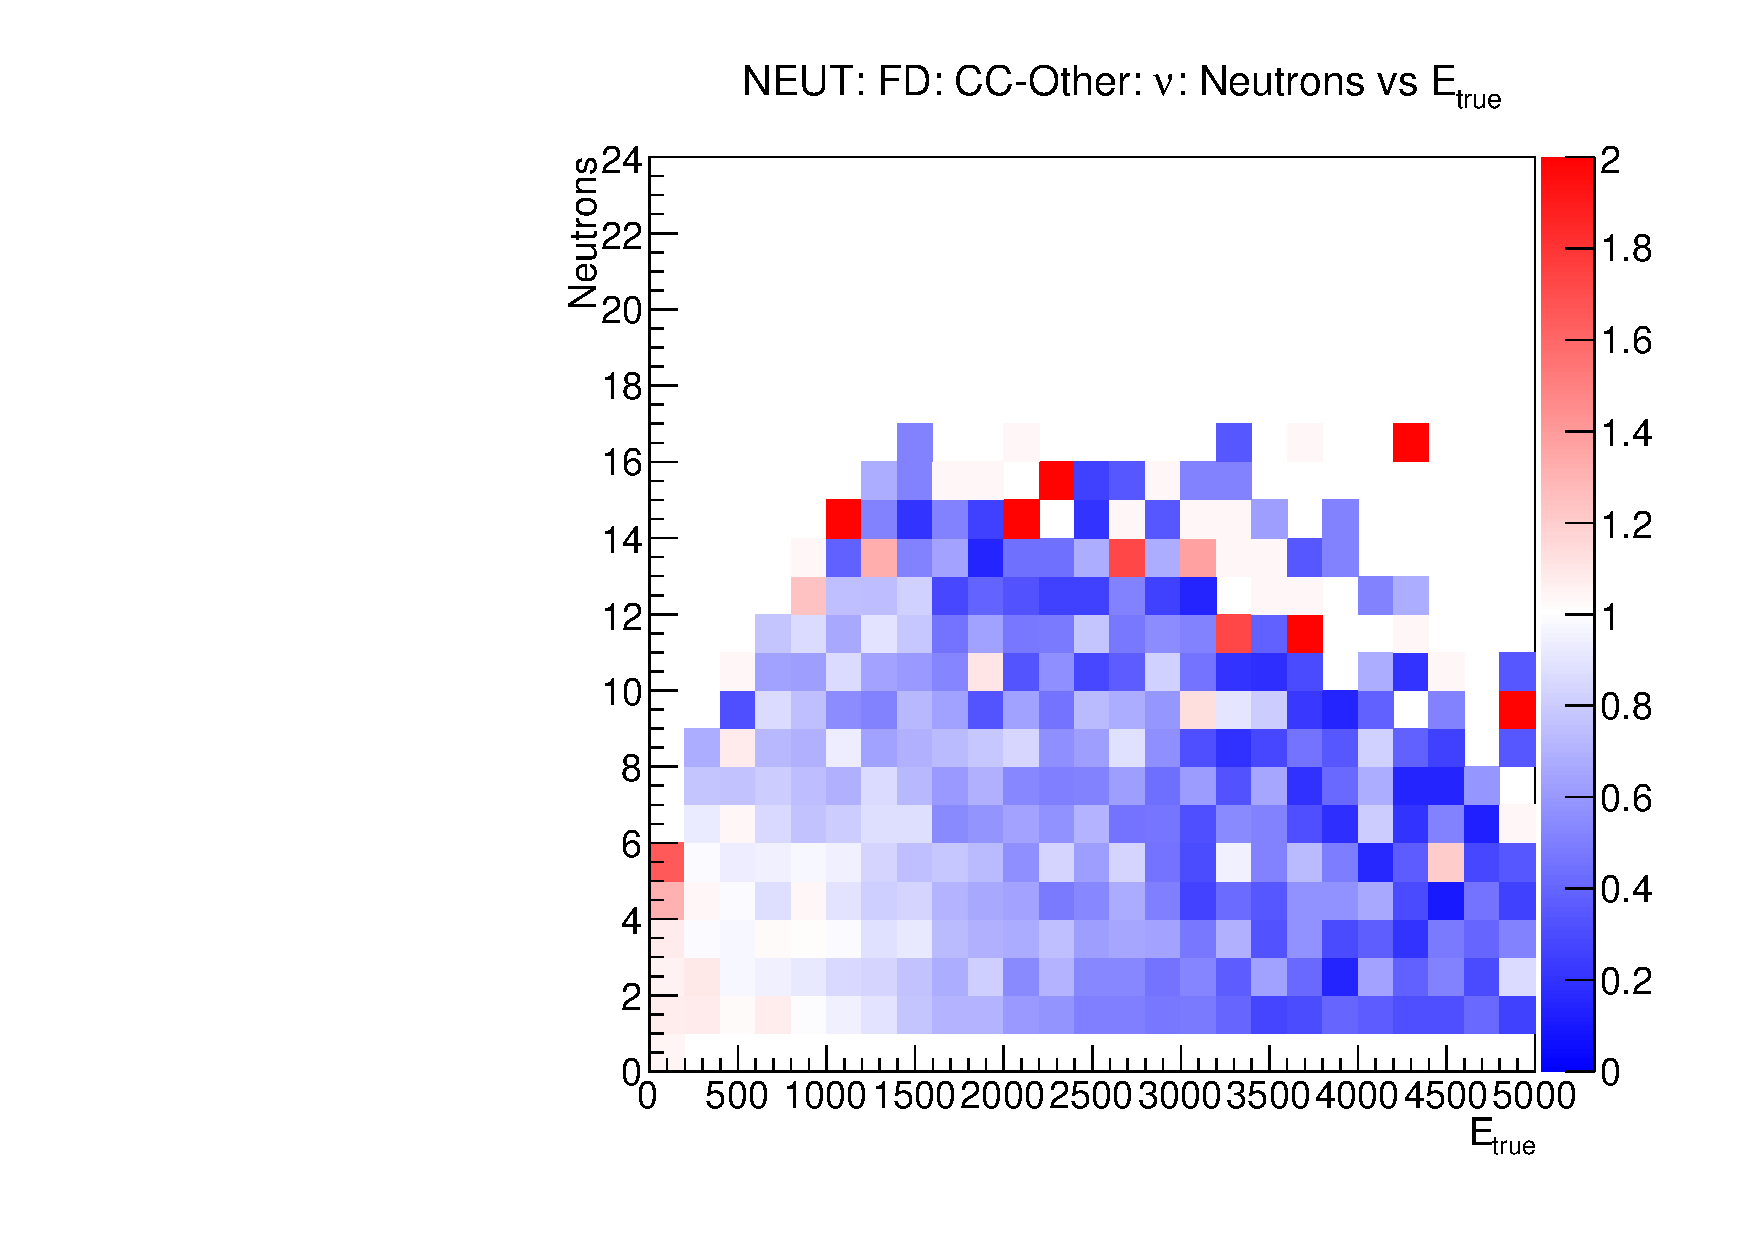
\includegraphics[width=\textwidth]{nneutrons_v_total_ene/Nneutrons_Total_ENe_dis_NEUT_ND_FD_numu_norm.pdf}
\end{subfigure}
\begin{subfigure}[b]{0.32\textwidth}
  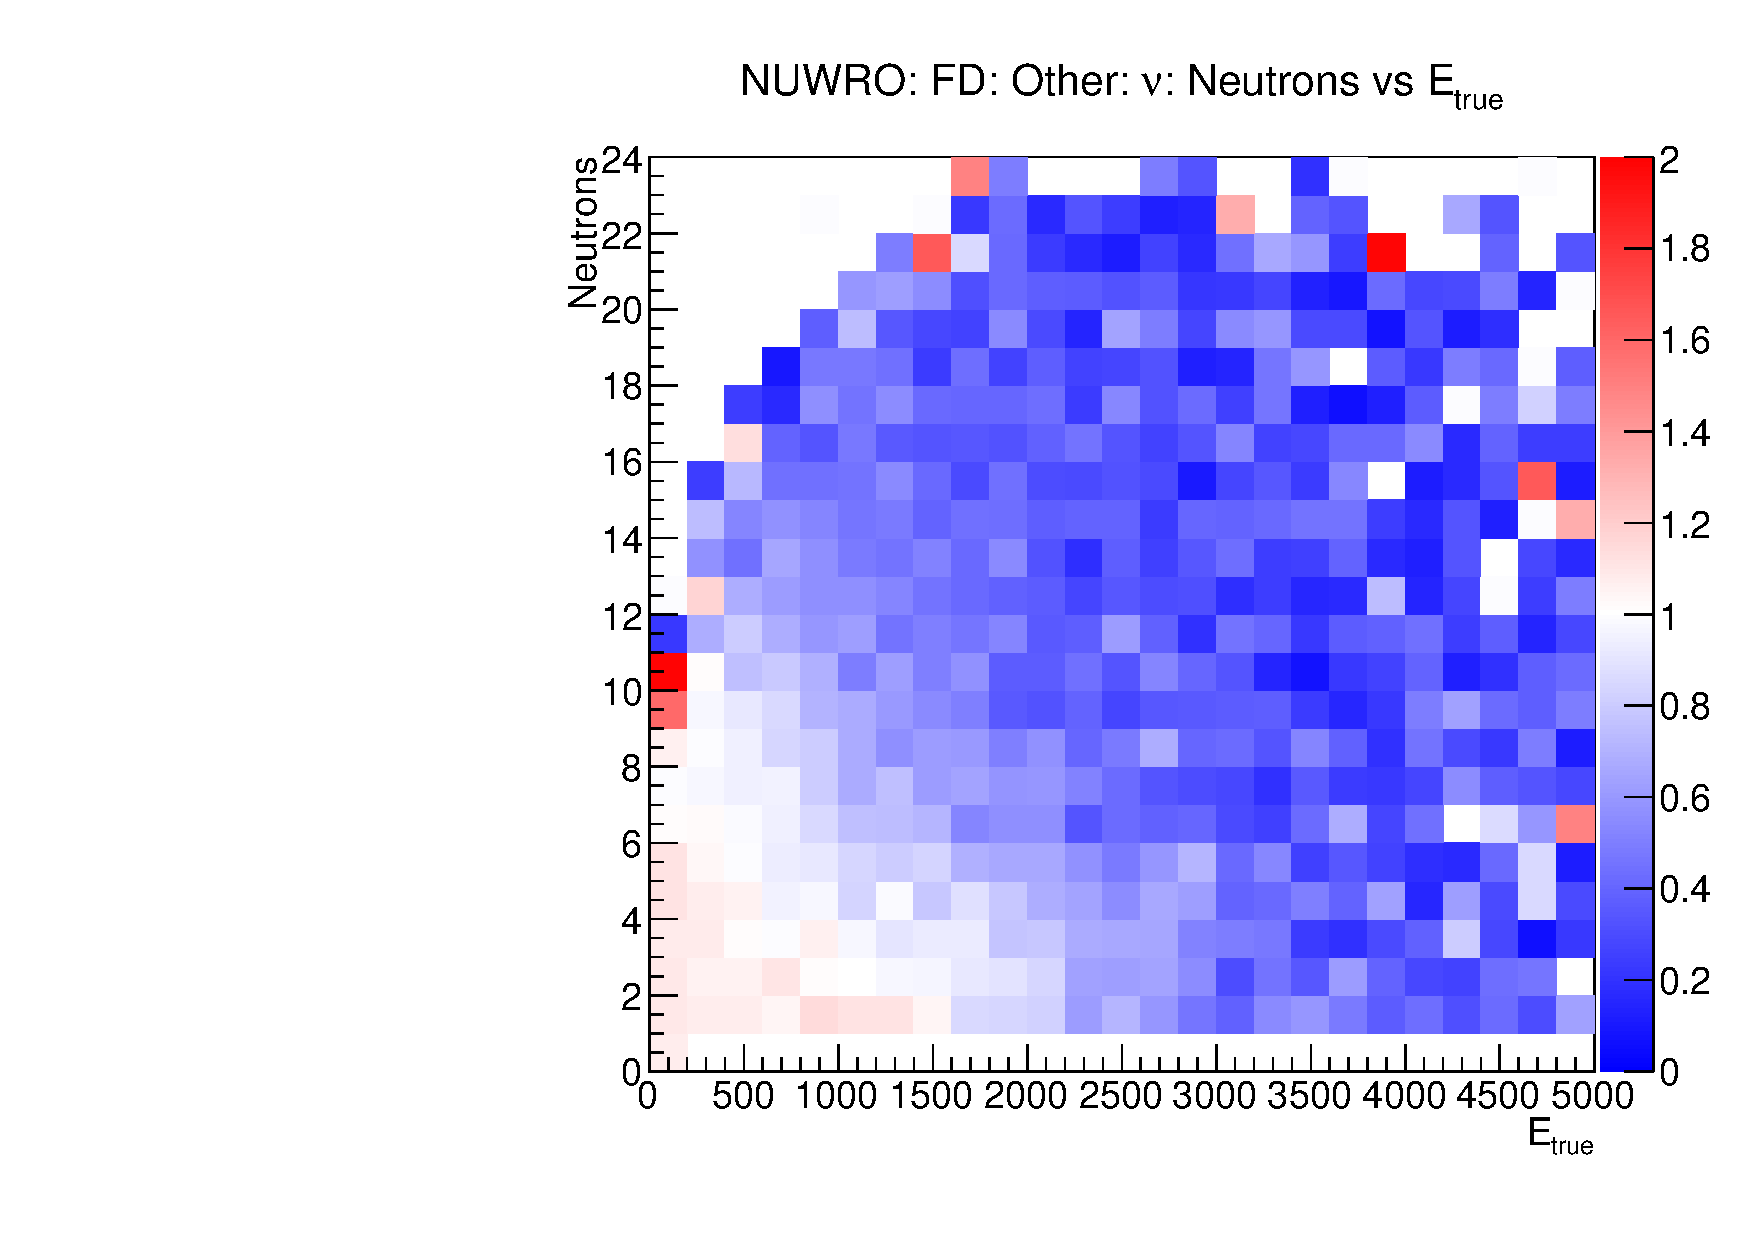
\includegraphics[width=\textwidth]{nneutrons_v_total_ene/Nneutrons_Total_ENe_dis_NUWRO_ND_FD_numu_norm.pdf}
\end{subfigure}
\end{figure}

\begin{figure}[!htb]
\centering
\begin{subfigure}[b]{0.32\textwidth}
  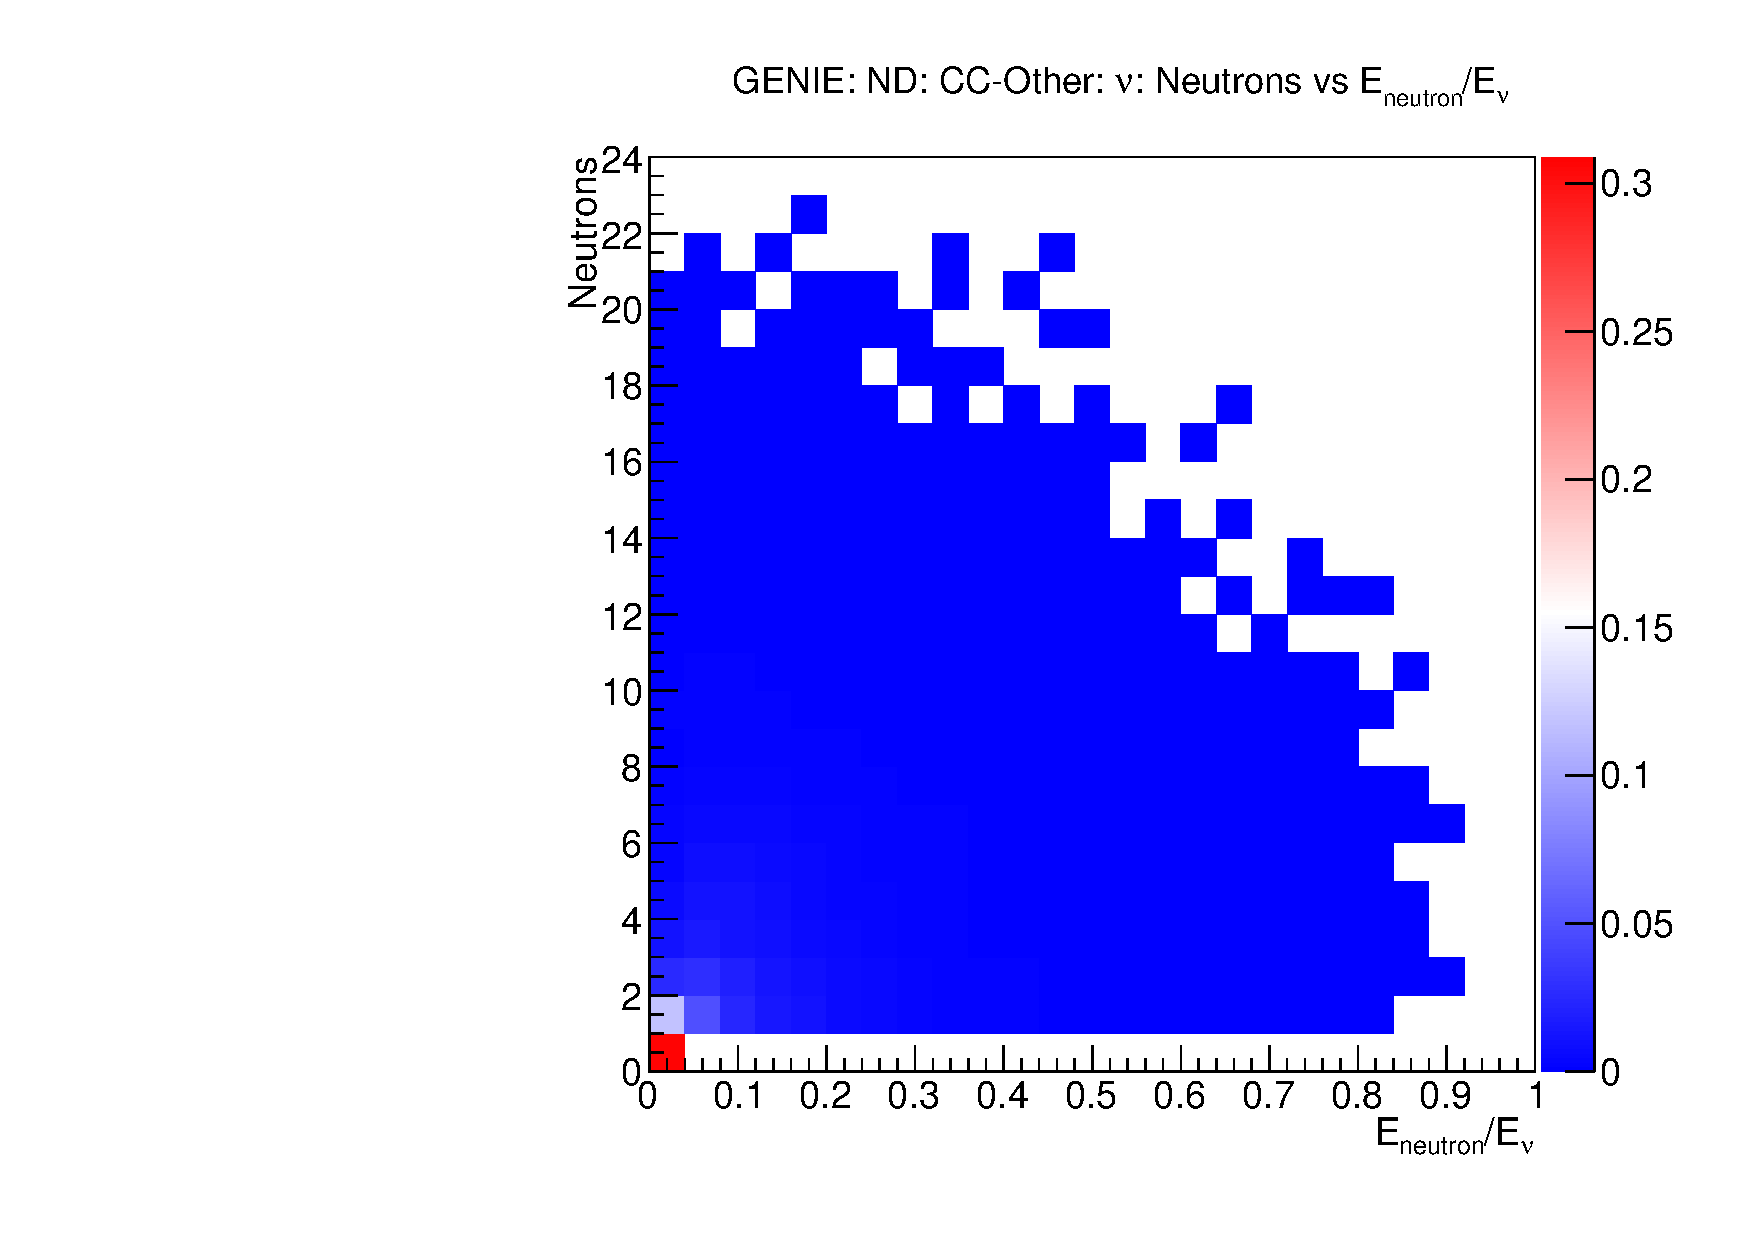
\includegraphics[width=\textwidth]{nneutrons_ene_enu/Nneutrons_Enu_true_dis_GENIE_ND_numu_norm.pdf}
\end{subfigure}
\begin{subfigure}[b]{0.32\textwidth}
  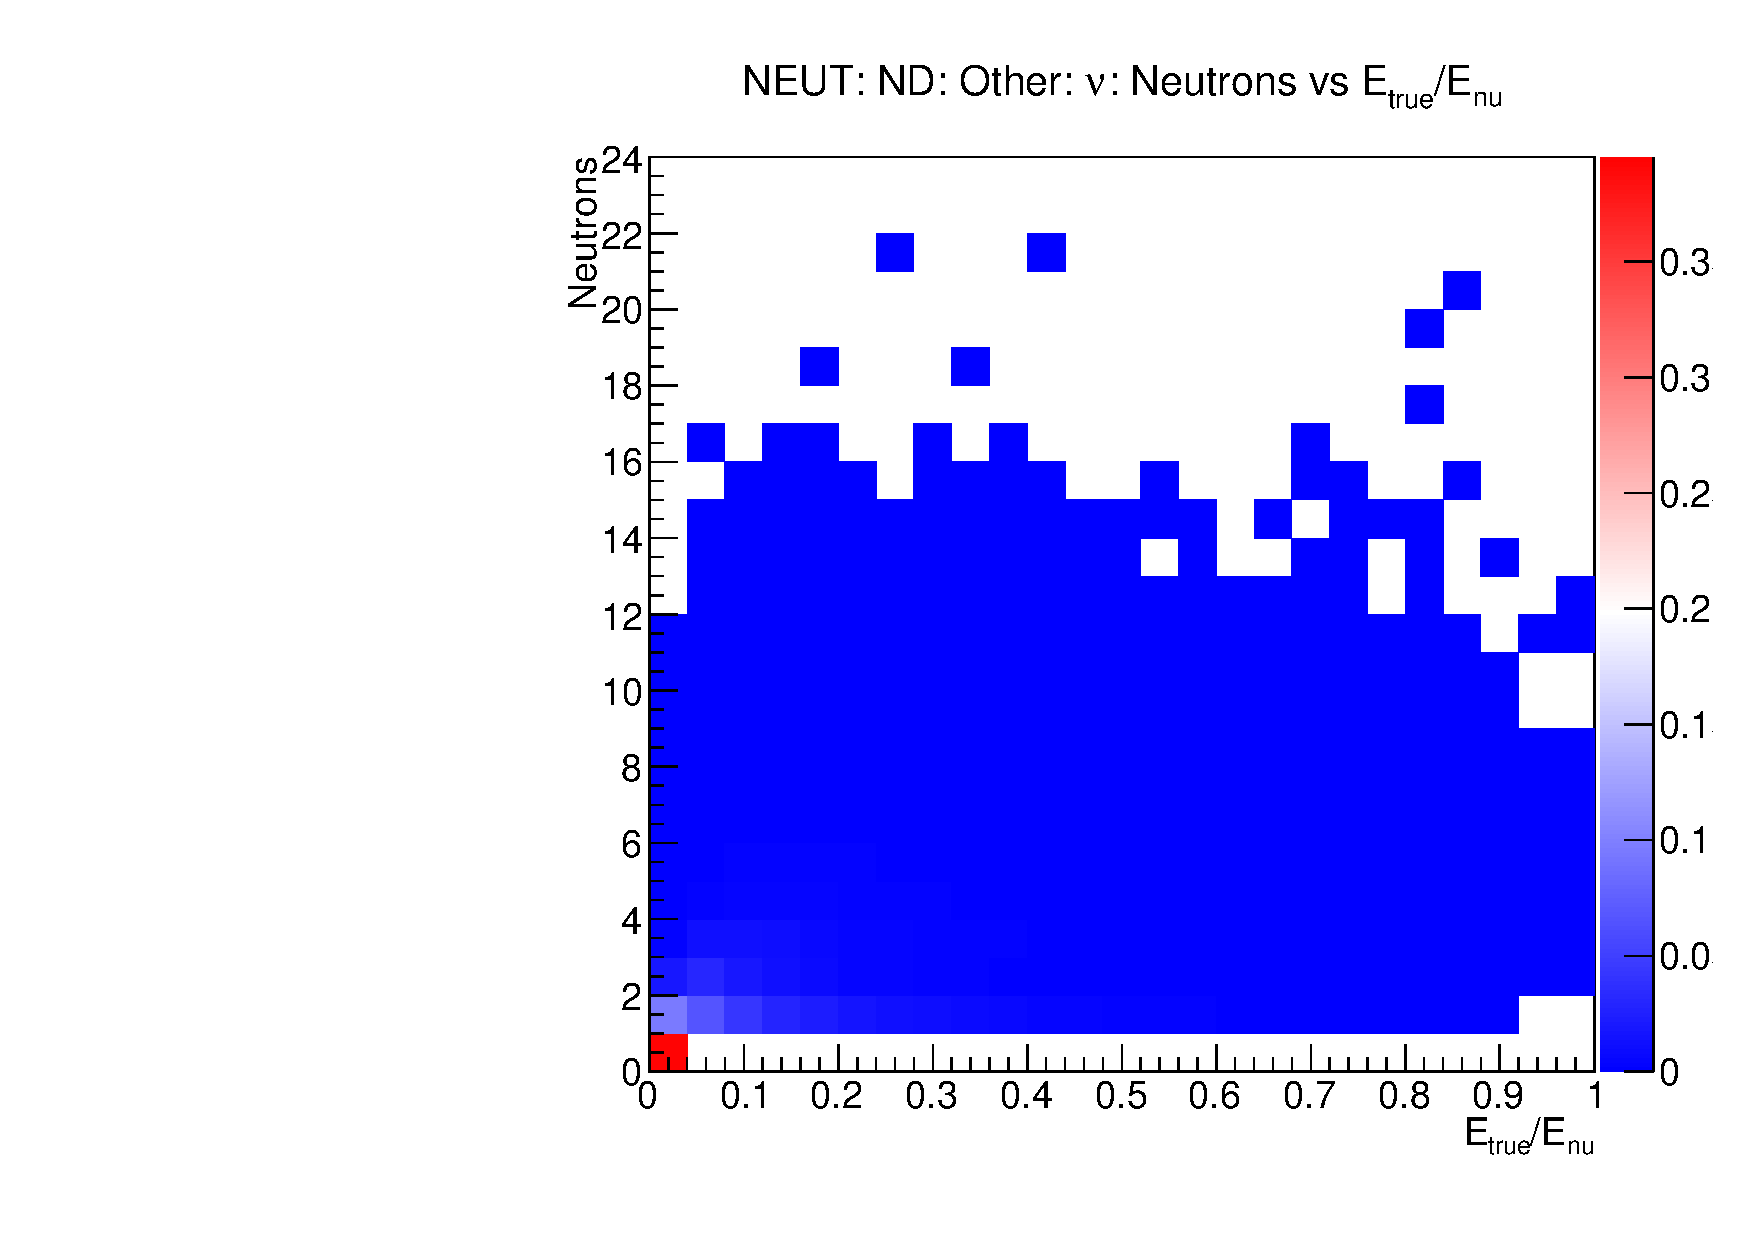
\includegraphics[width=\textwidth]{nneutrons_ene_enu/Nneutrons_Enu_true_dis_NEUT_ND_numu_norm.pdf}
\end{subfigure}
\begin{subfigure}[b]{0.32\textwidth}
  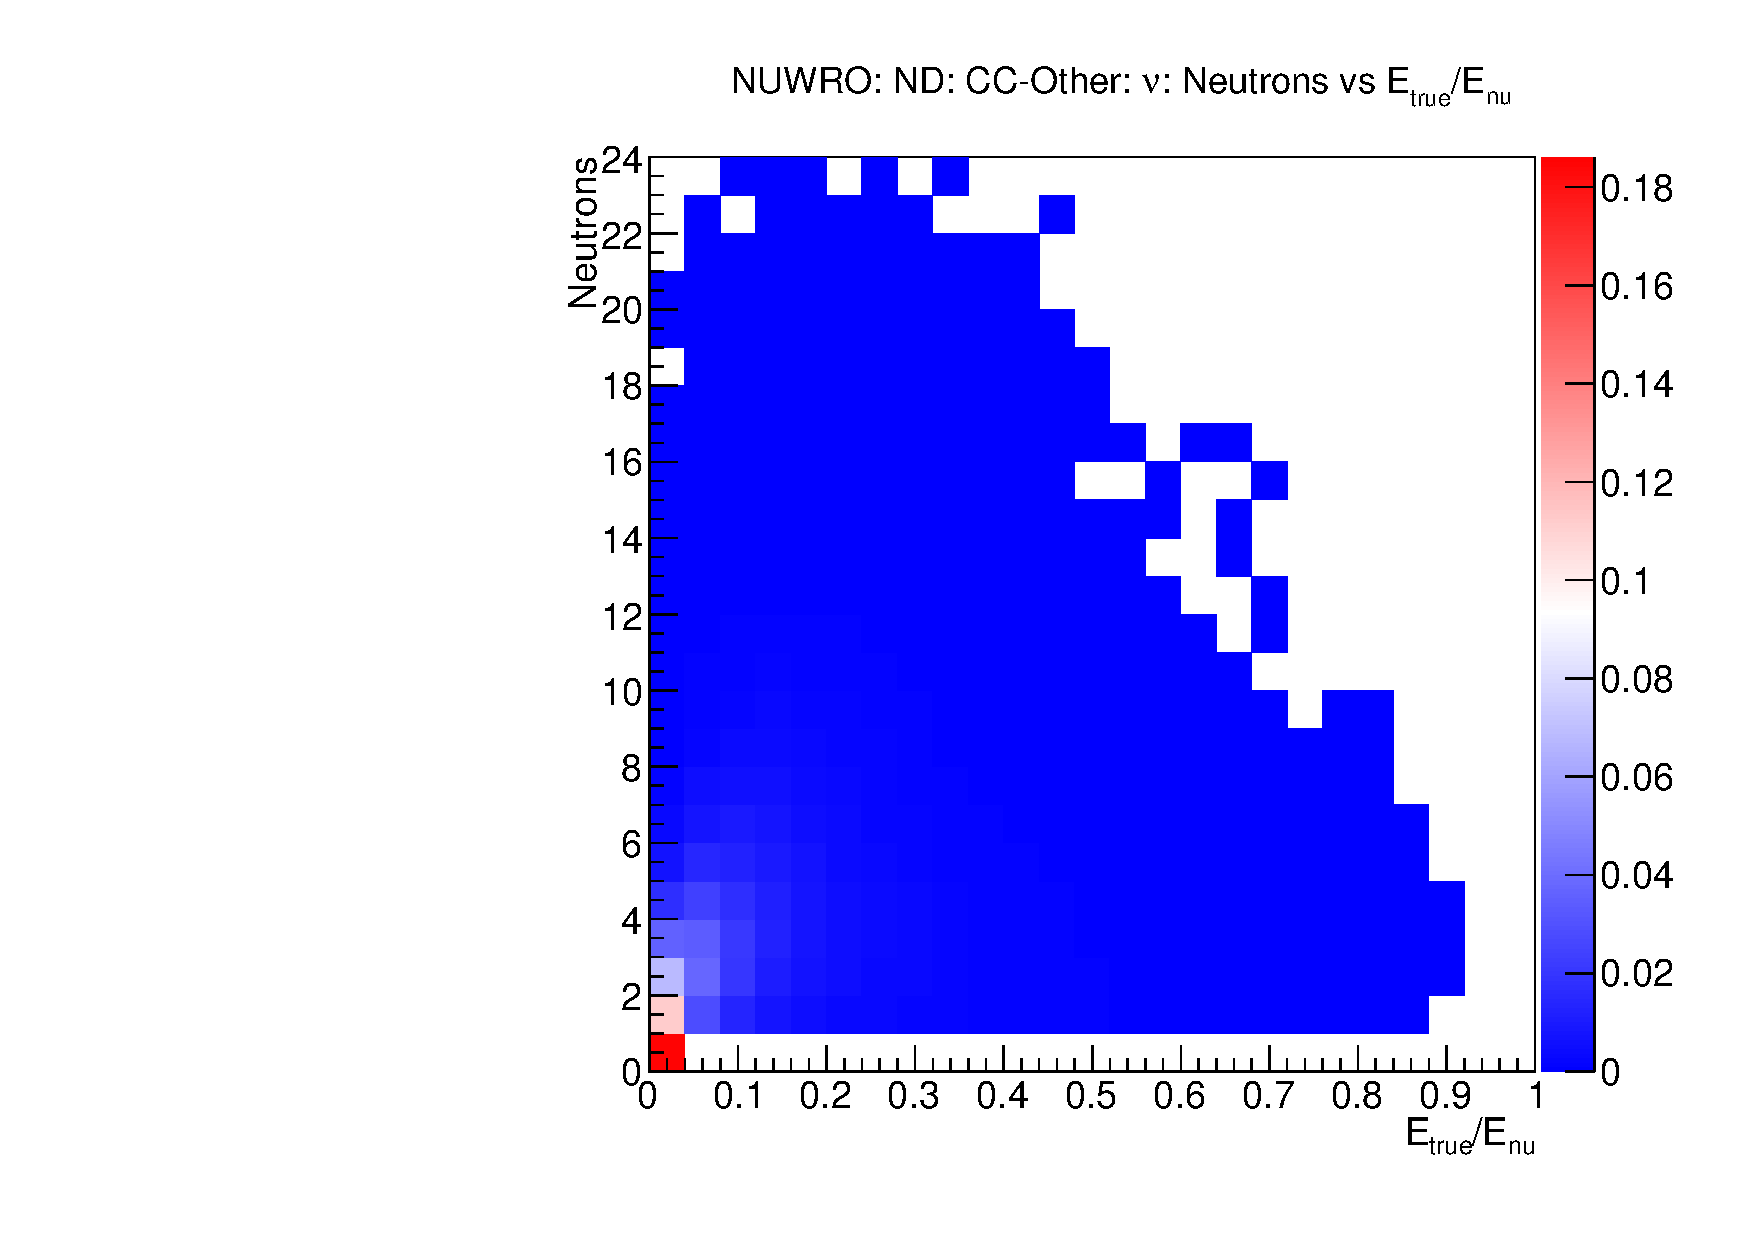
\includegraphics[width=\textwidth]{nneutrons_ene_enu/Nneutrons_Enu_true_dis_NUWRO_ND_numu_norm.pdf}
\end{subfigure}
\end{figure}
\FloatBarrier

\subsection{$\bar{\nu}$ Plots}


\subsubsection{CCQE}

\begin{figure}[!htb]
\centering
\begin{subfigure}[b]{0.32\textwidth}
  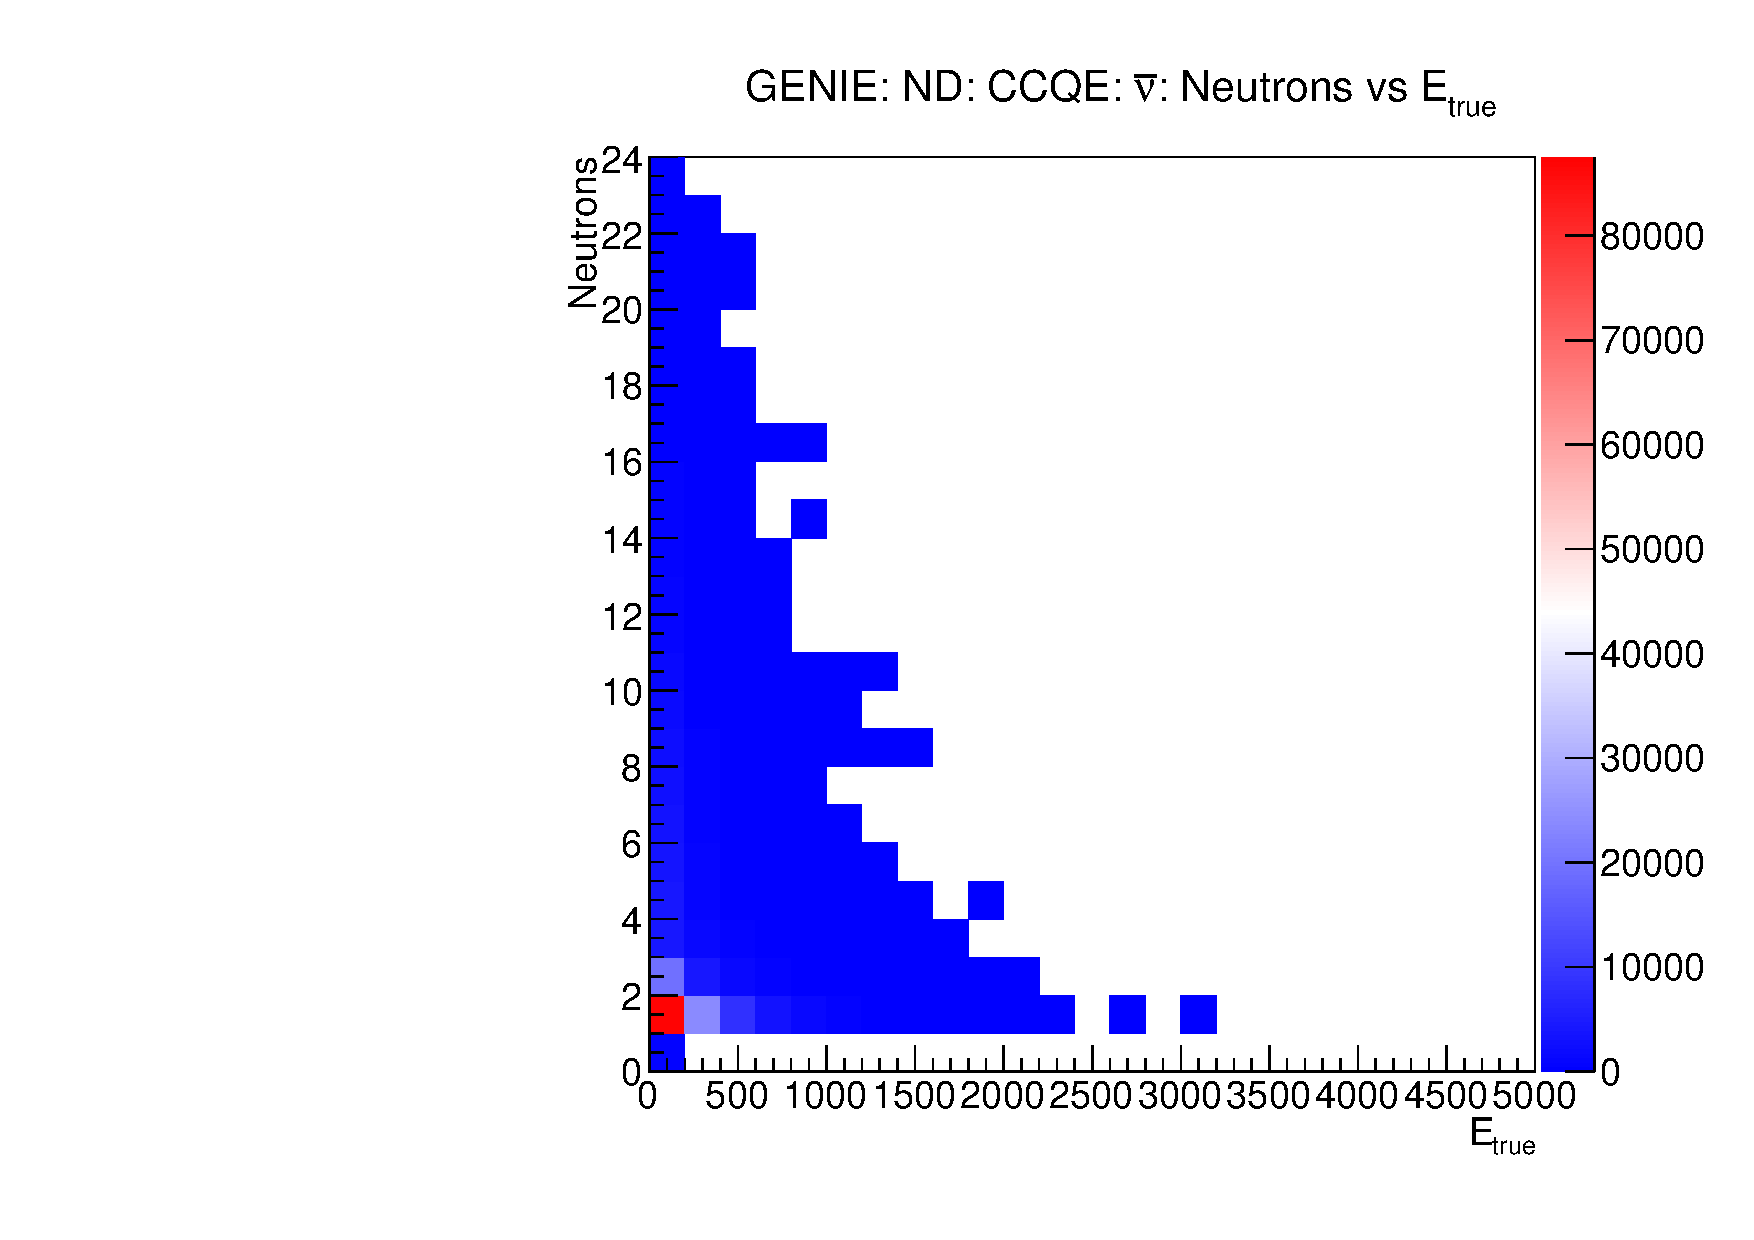
\includegraphics[width=\textwidth]{nneutrons_v_total_ene/Nneutrons_Total_ENe_ccqe_GENIE_ND_numub.pdf}
\end{subfigure}
\begin{subfigure}[b]{0.32\textwidth}
  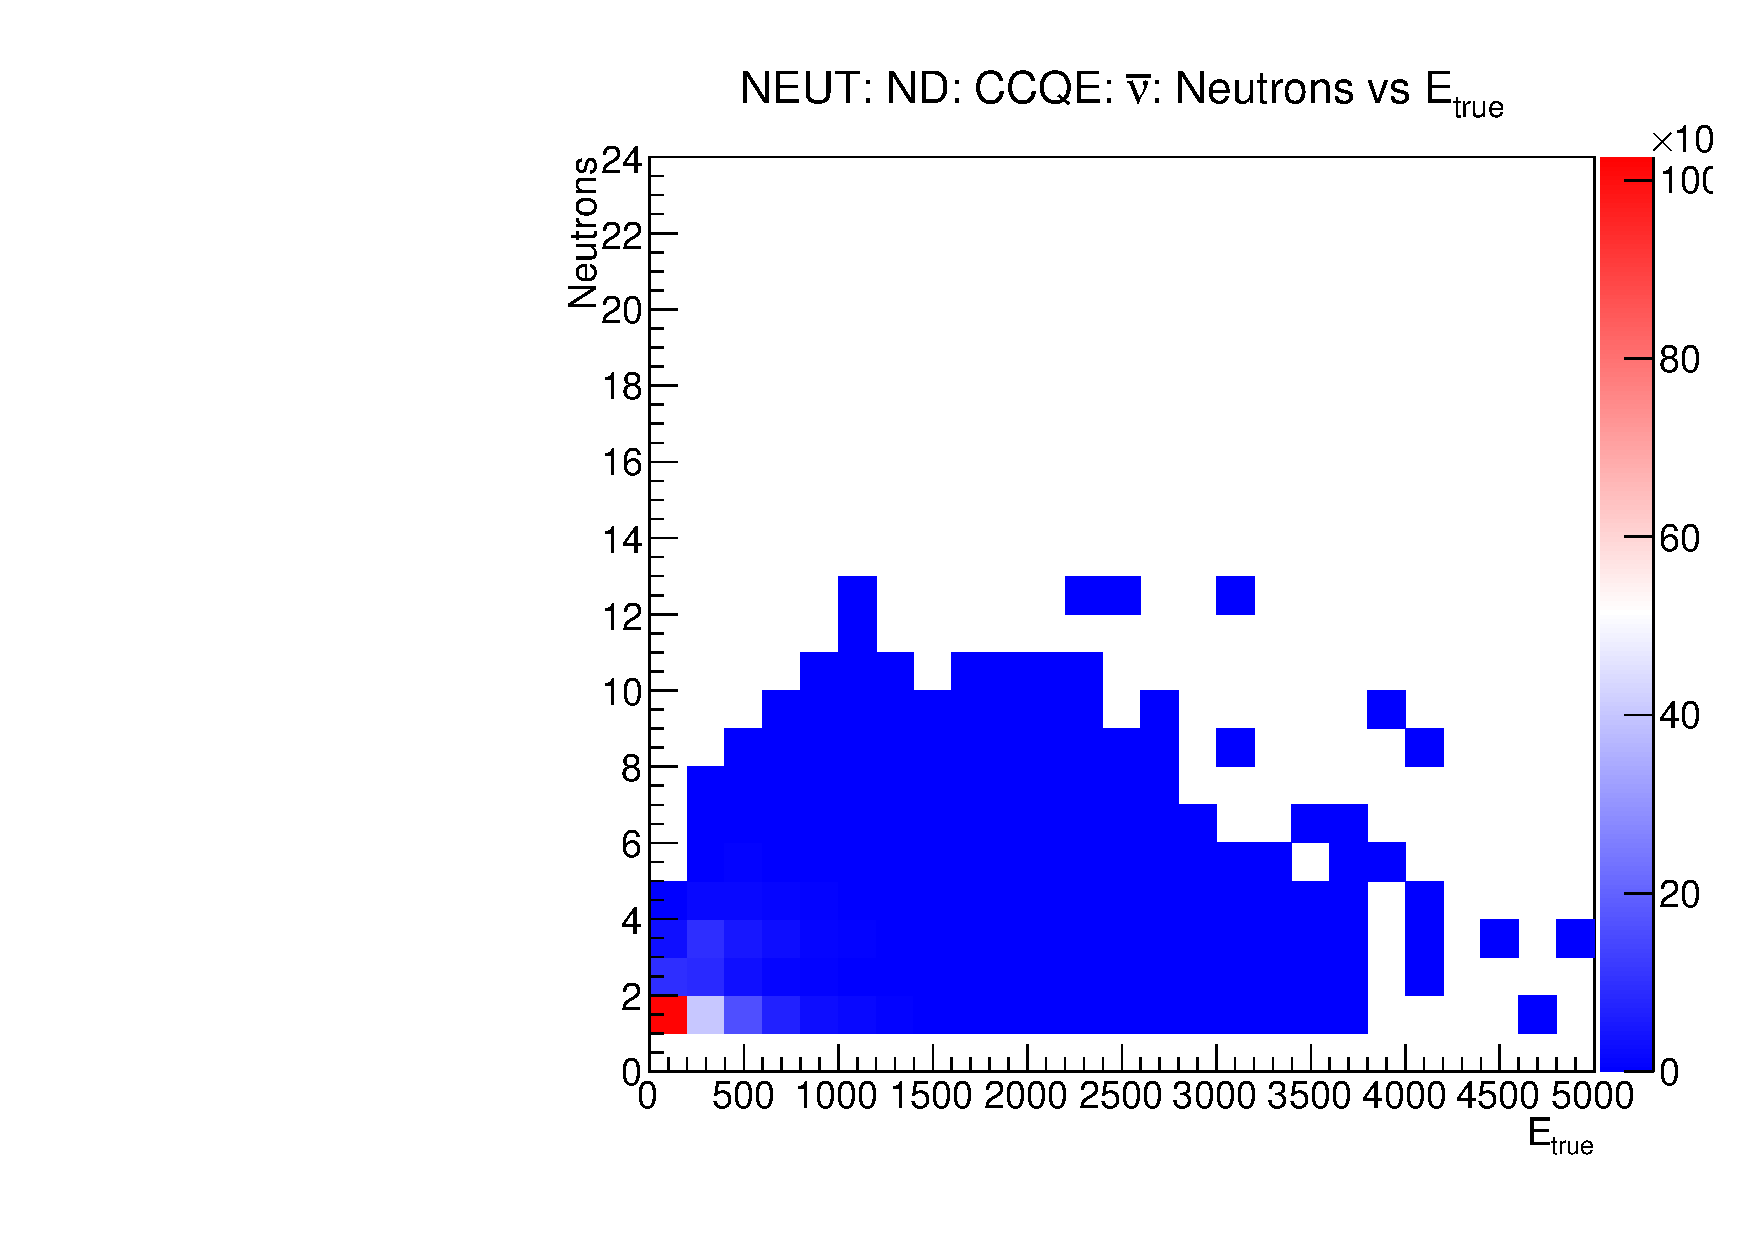
\includegraphics[width=\textwidth]{nneutrons_v_total_ene/Nneutrons_Total_ENe_ccqe_NEUT_ND_numub.pdf}
\end{subfigure}
\begin{subfigure}[b]{0.32\textwidth}
  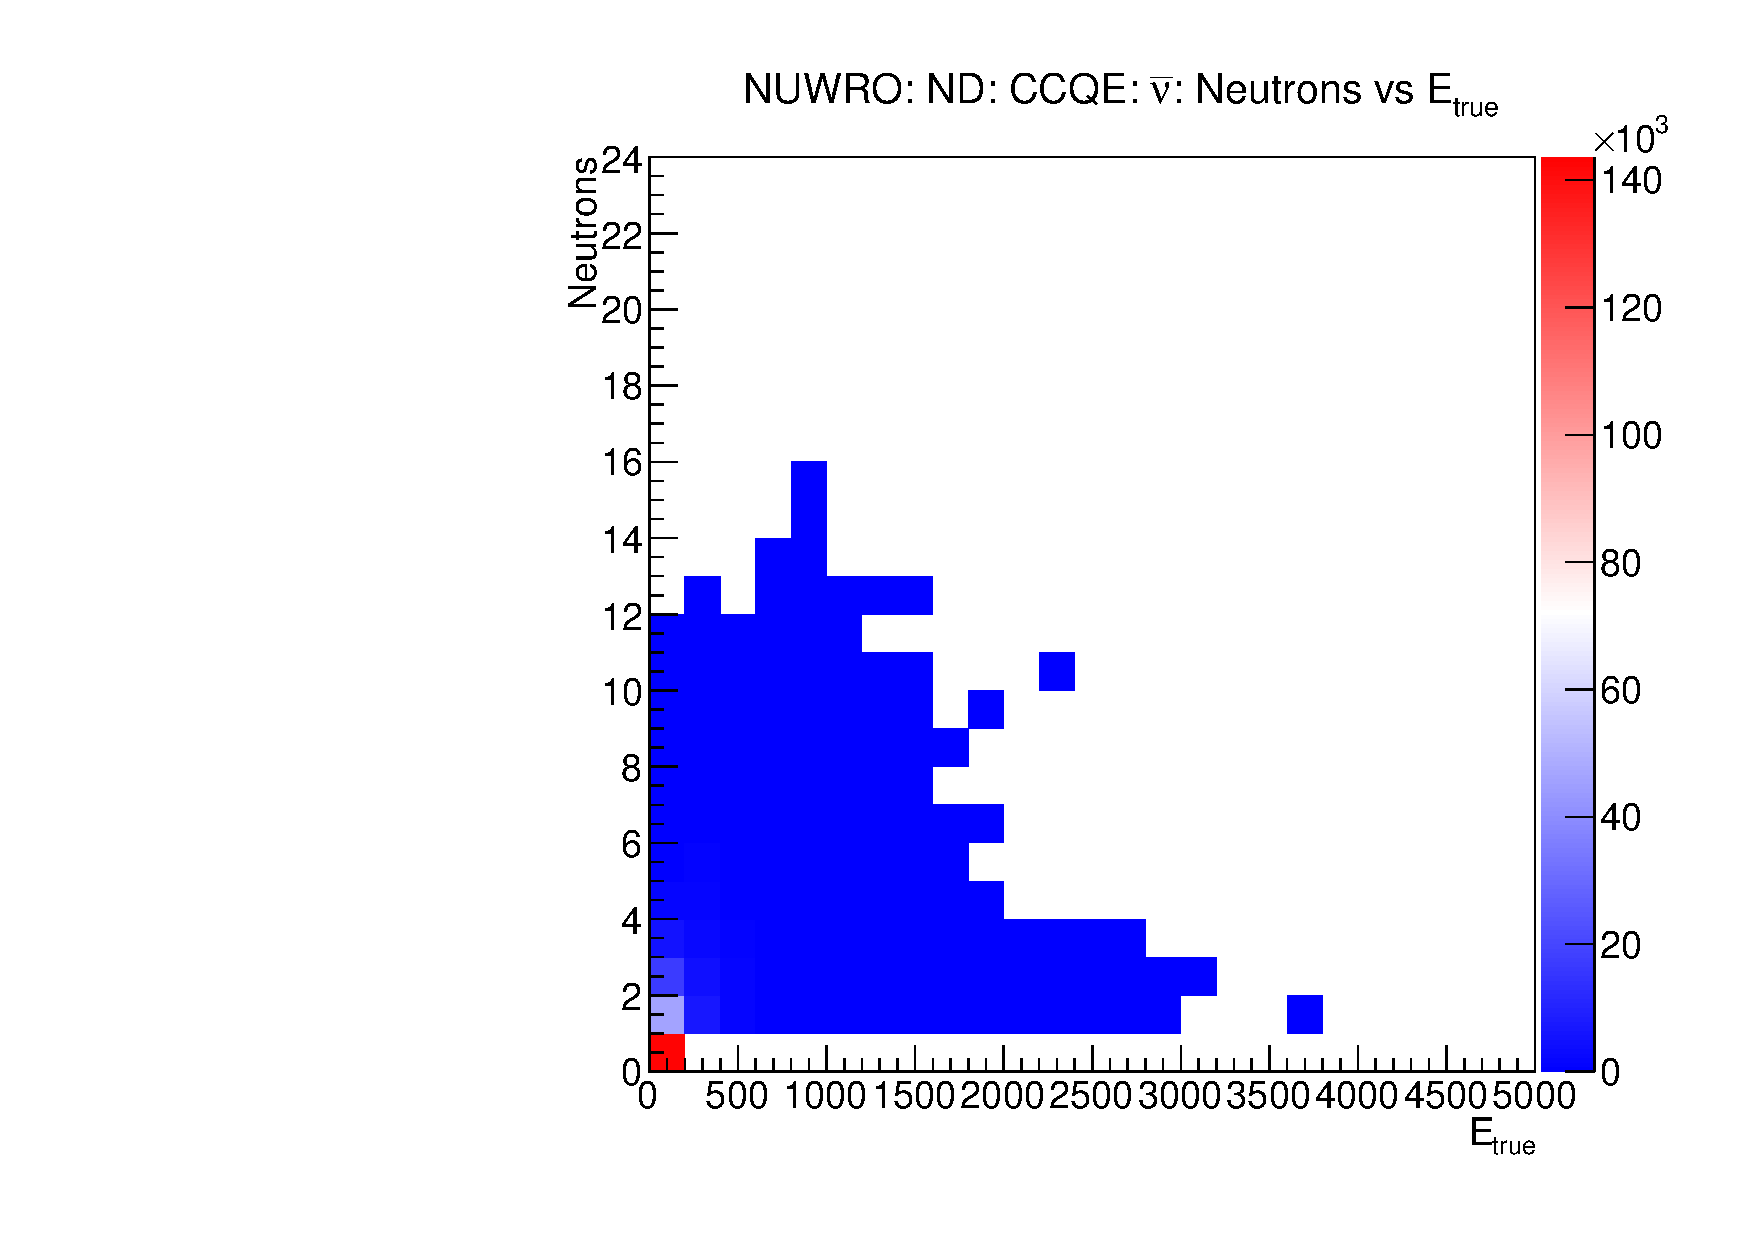
\includegraphics[width=\textwidth]{nneutrons_v_total_ene/Nneutrons_Total_ENe_ccqe_NUWRO_ND_numub.pdf}
\end{subfigure}
\end{figure}

\begin{figure}[!htb]
\centering
\begin{subfigure}[b]{0.32\textwidth}
  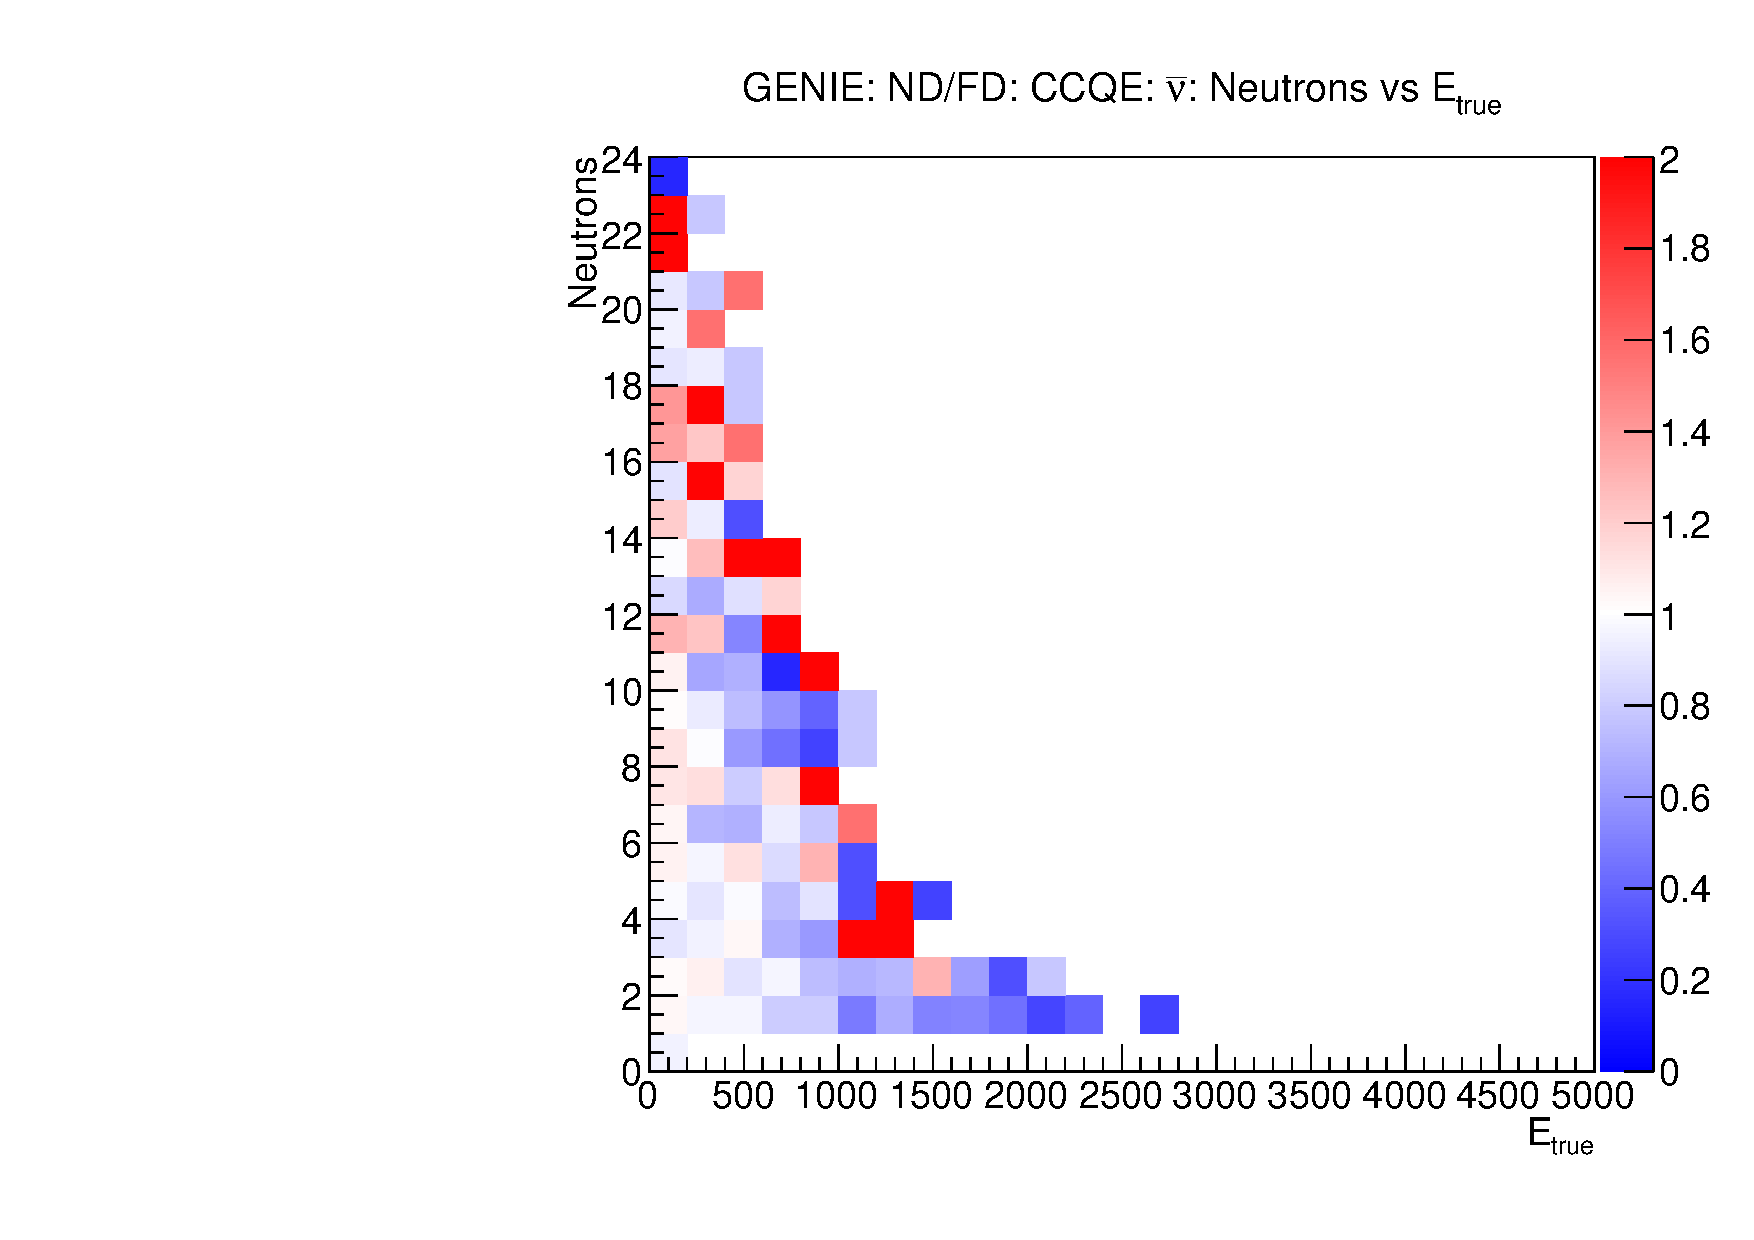
\includegraphics[width=\textwidth]{nneutrons_v_total_ene/Nneutrons_Total_ENe_ccqe_GENIE_ND_FD_numub_norm.pdf}
\end{subfigure}
\begin{subfigure}[b]{0.32\textwidth}
  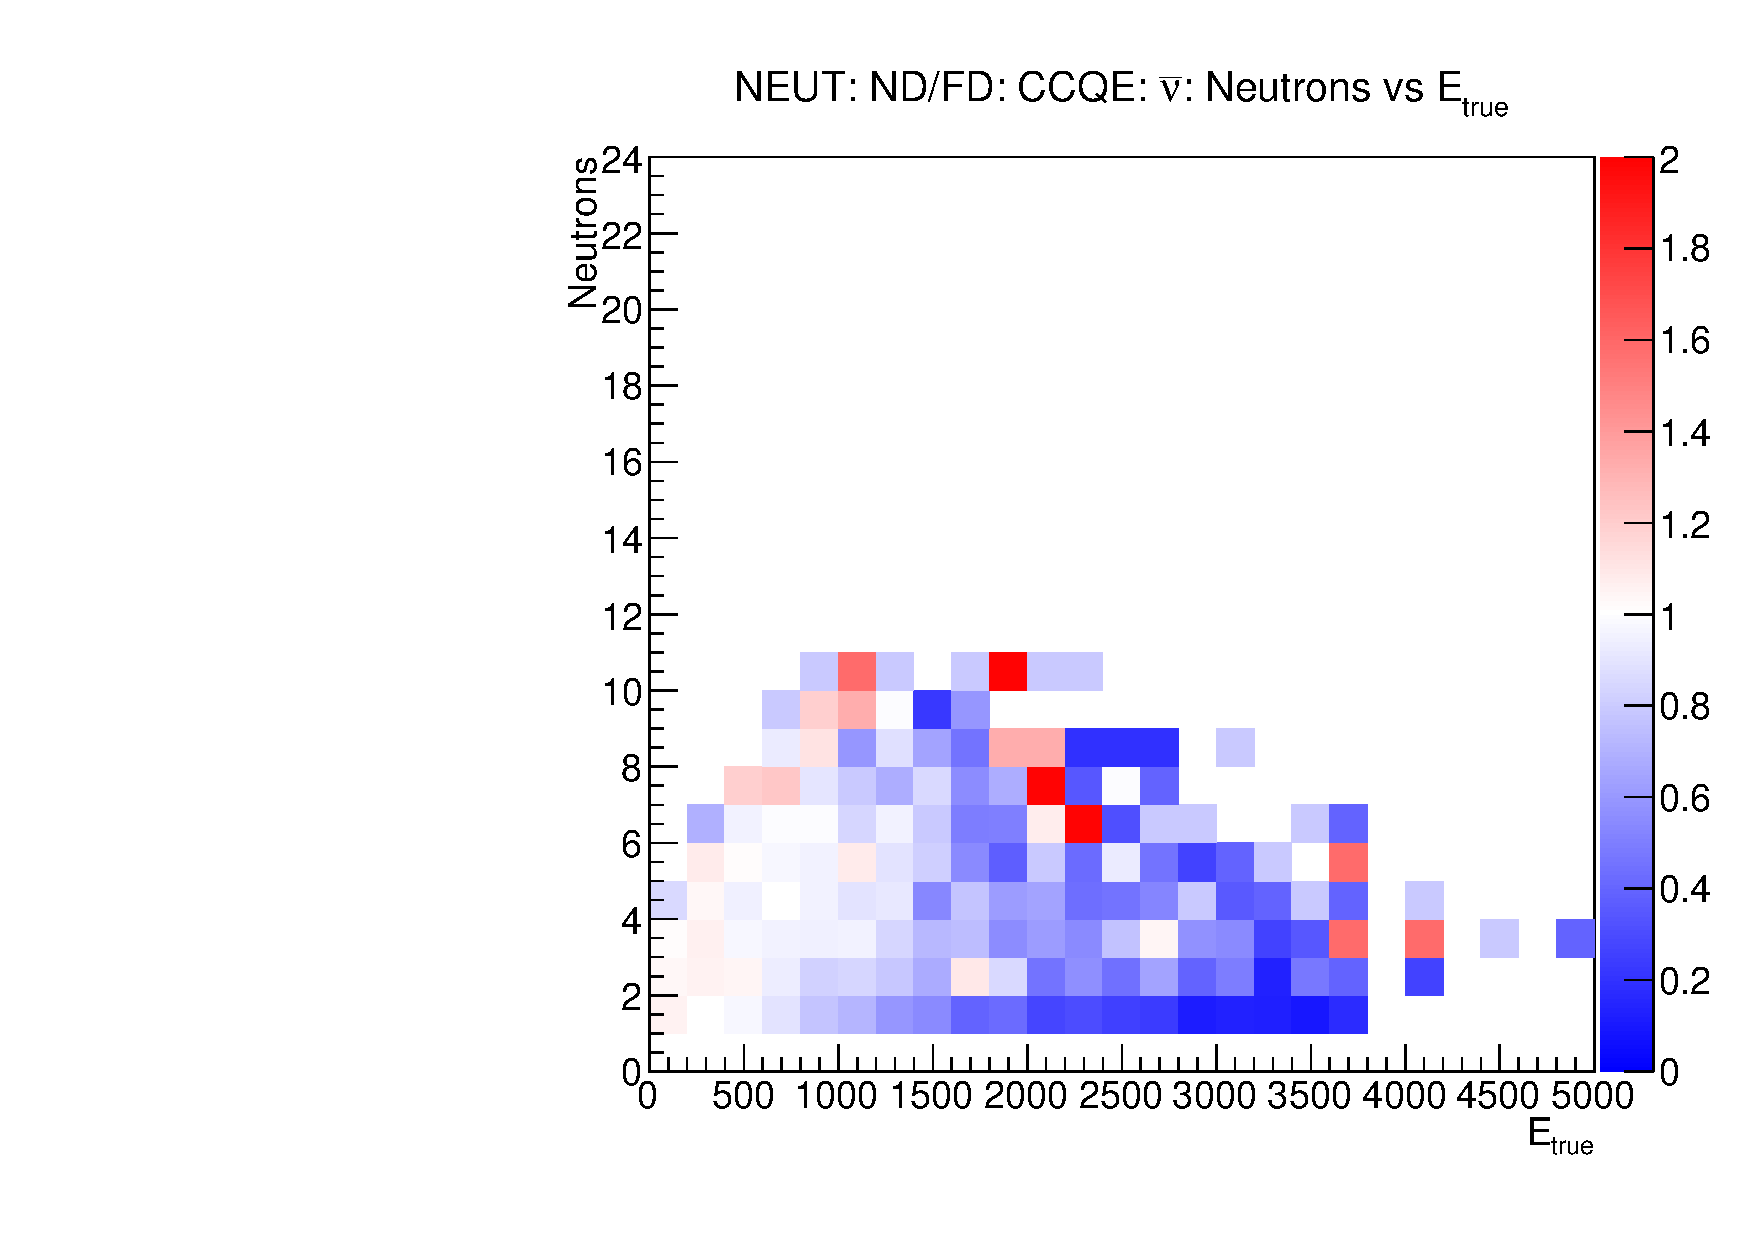
\includegraphics[width=\textwidth]{nneutrons_v_total_ene/Nneutrons_Total_ENe_ccqe_NEUT_ND_FD_numub_norm.pdf}
\end{subfigure}
\begin{subfigure}[b]{0.32\textwidth}
  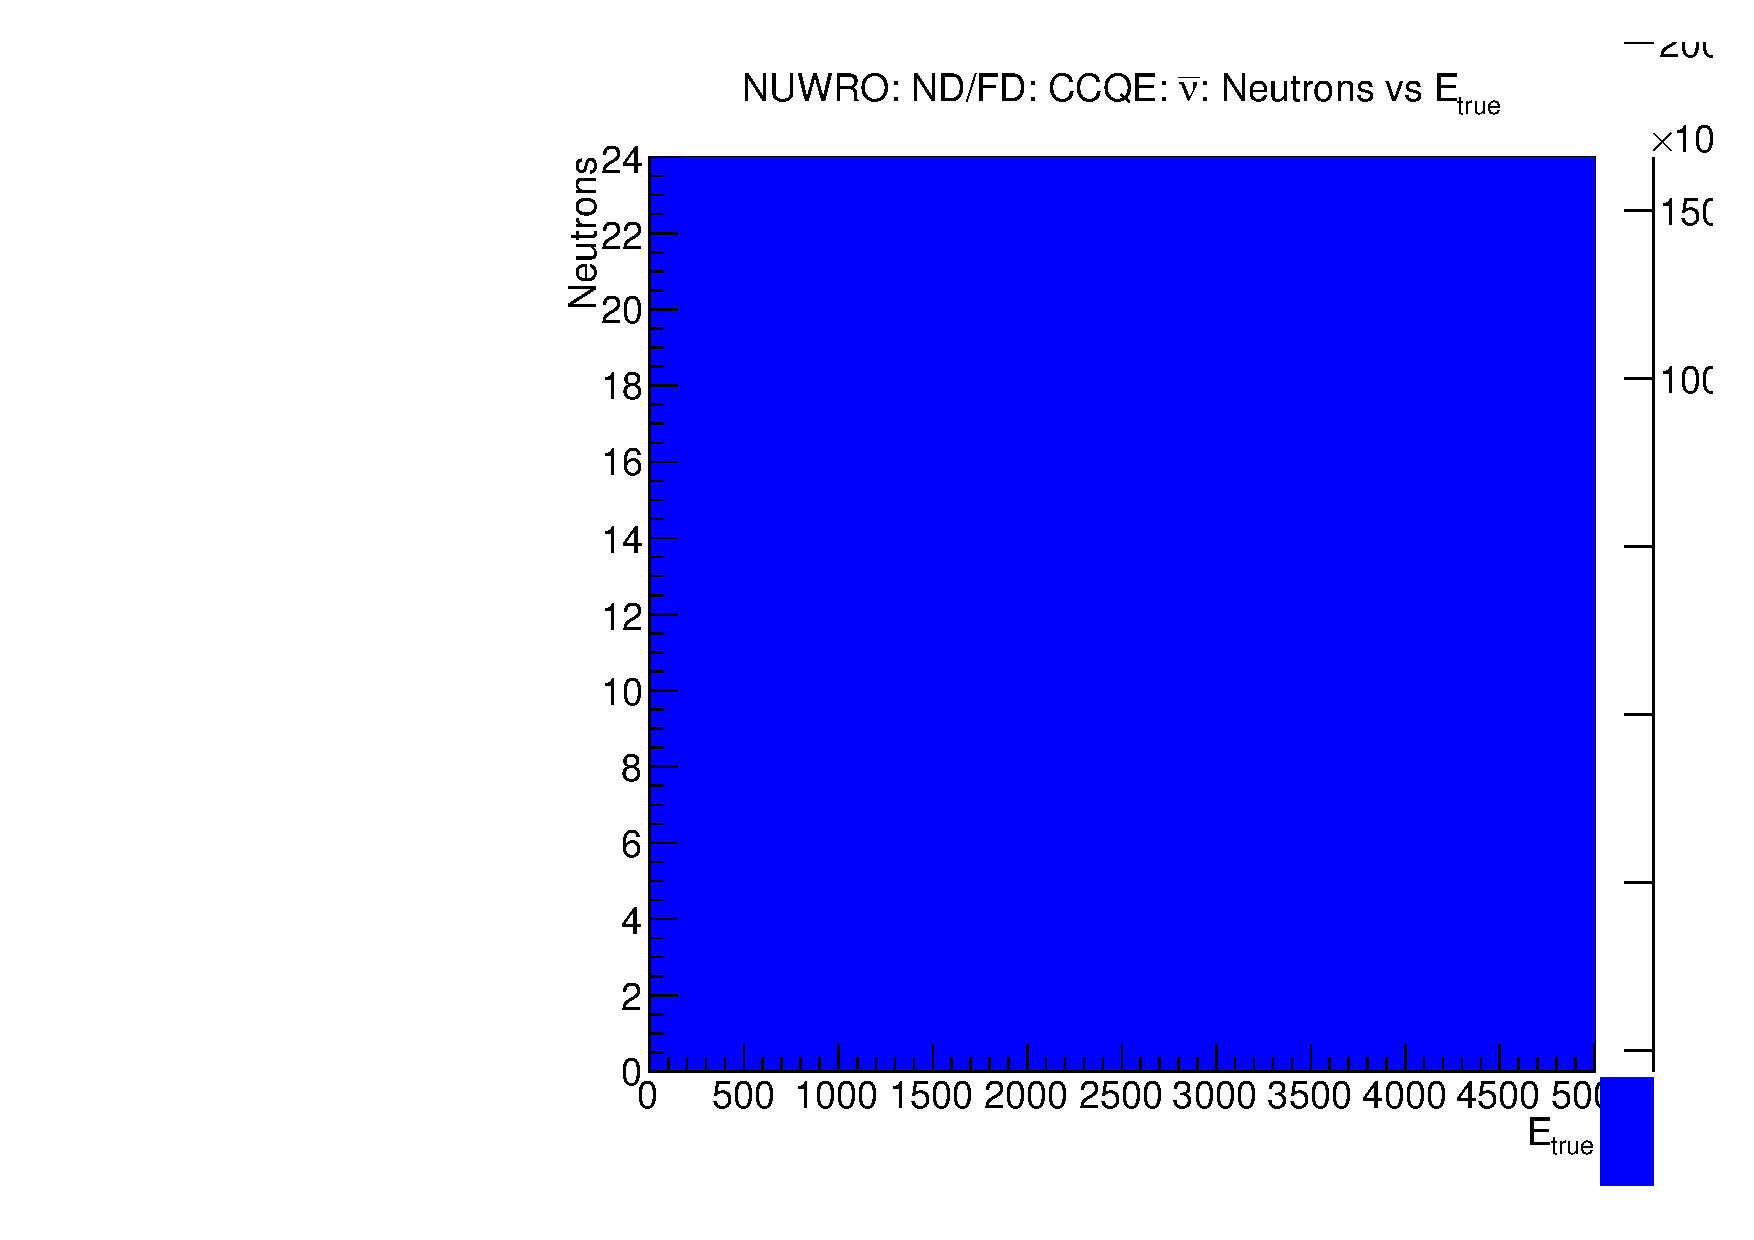
\includegraphics[width=\textwidth]{nneutrons_v_total_ene/Nneutrons_Total_ENe_ccqe_NUWRO_ND_FD_numub_norm.pdf}
\end{subfigure}
\end{figure}

\begin{figure}[!htb]
\centering
\begin{subfigure}[b]{0.32\textwidth}
  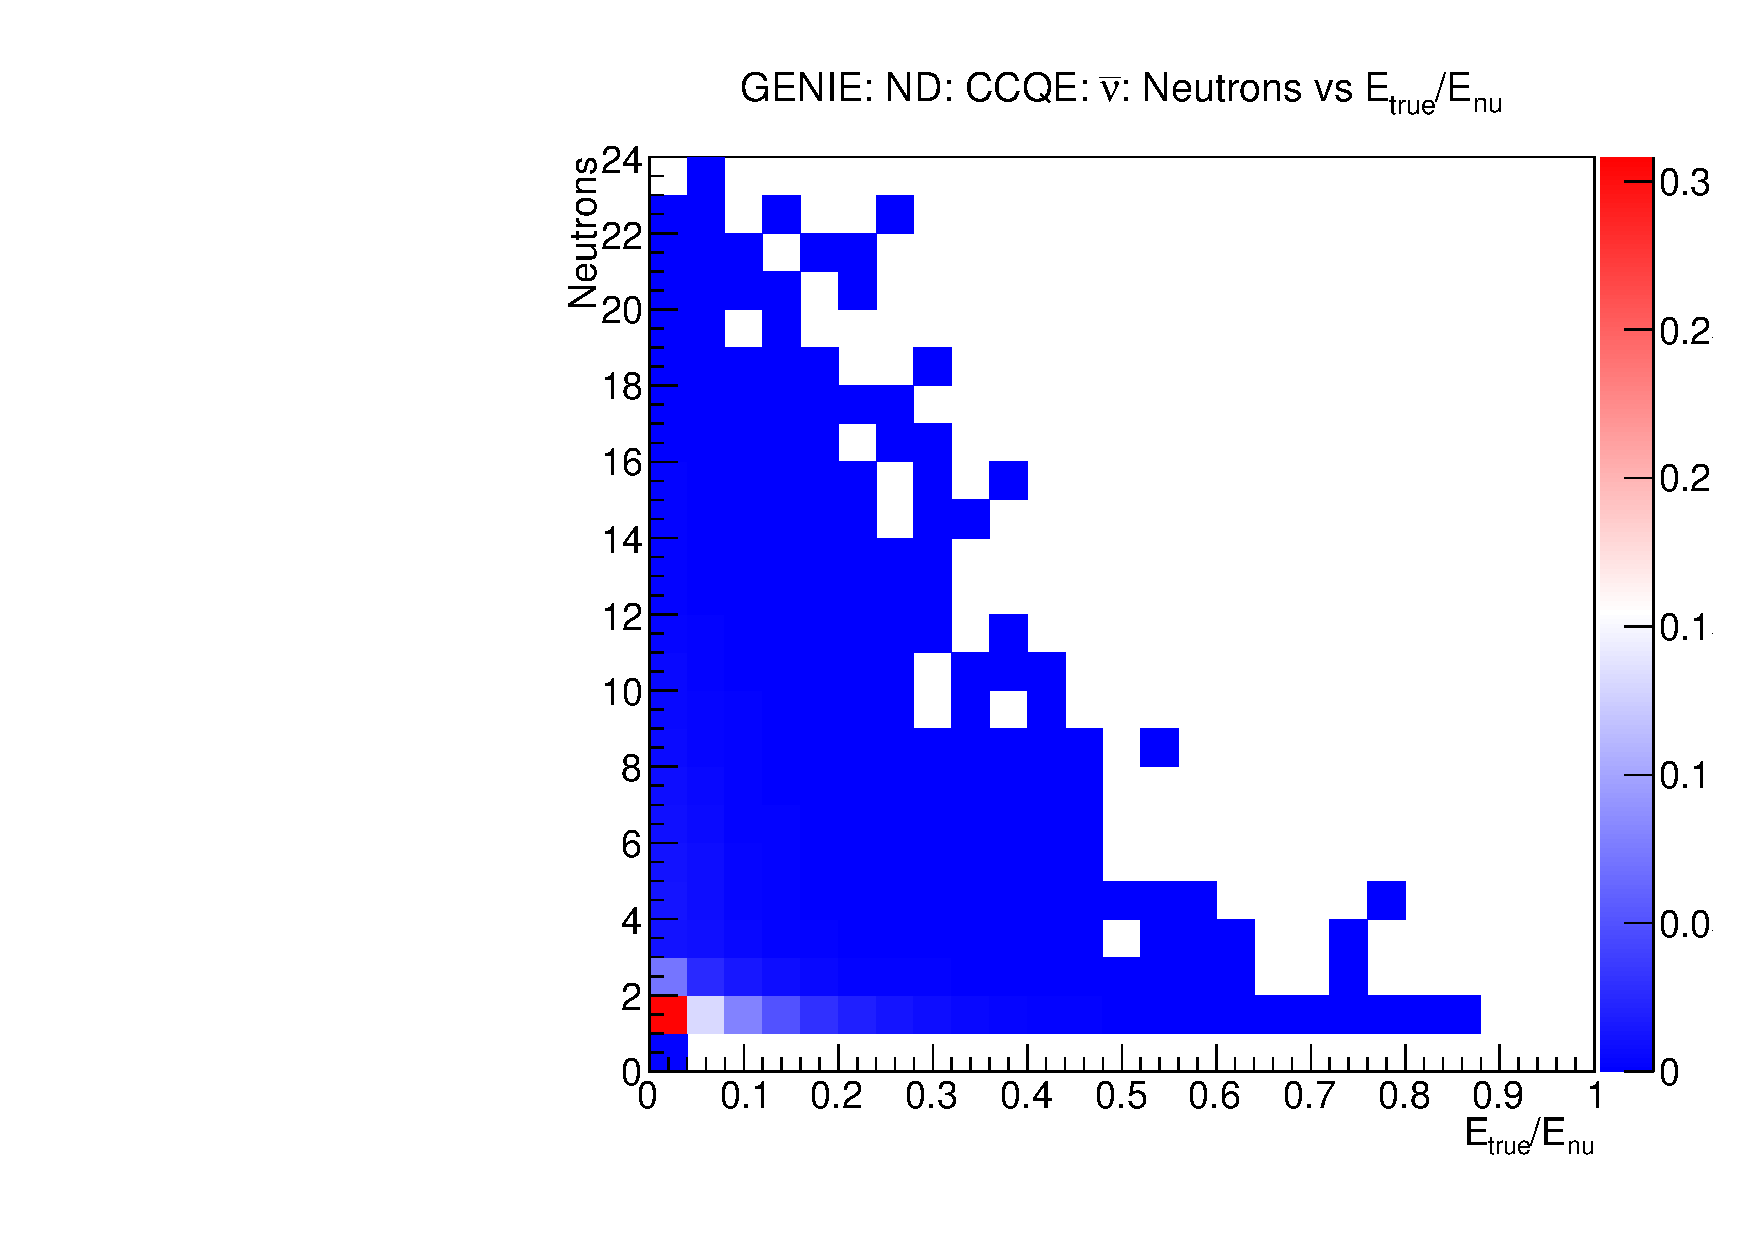
\includegraphics[width=\textwidth]{nneutrons_ene_enu/Nneutrons_Enu_true_ccqe_GENIE_ND_numub_norm.pdf}
\end{subfigure}
\begin{subfigure}[b]{0.32\textwidth}
  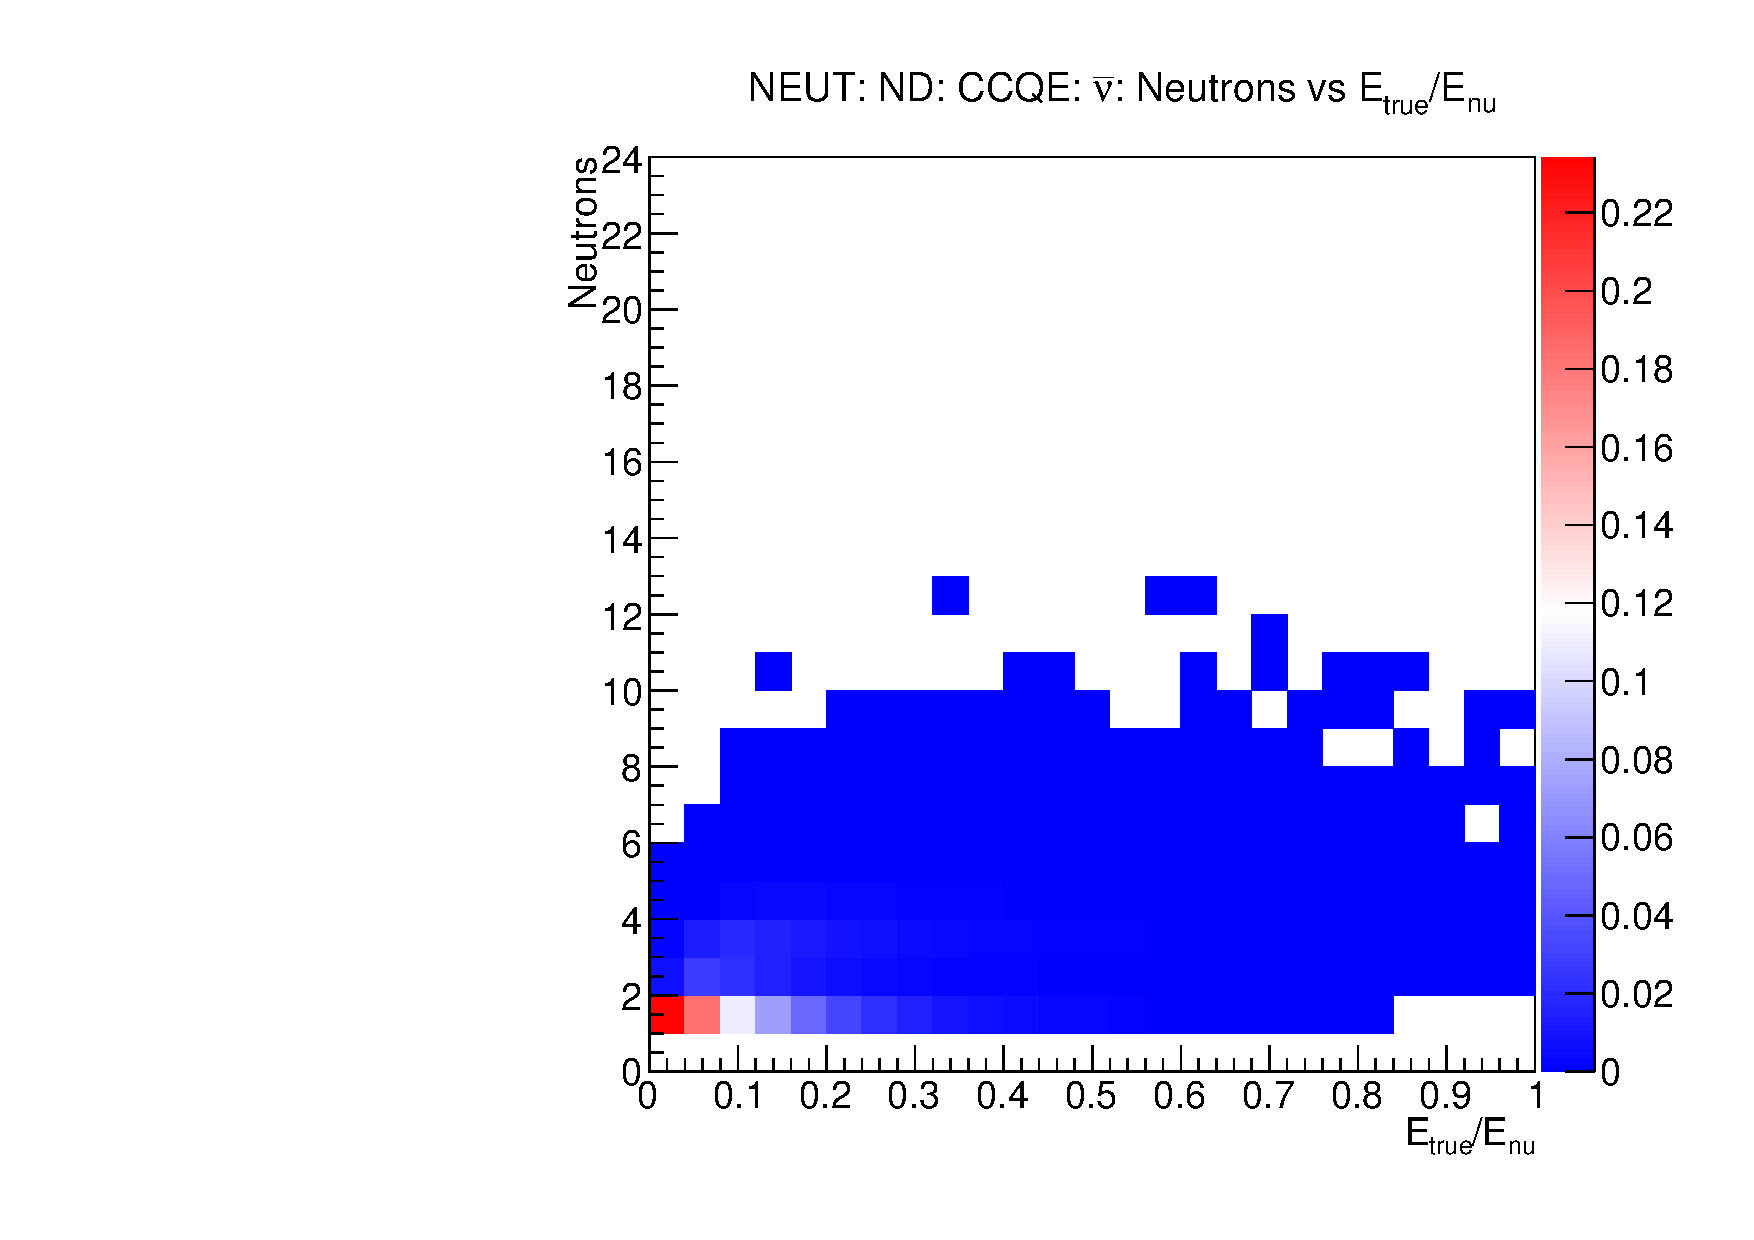
\includegraphics[width=\textwidth]{nneutrons_ene_enu/Nneutrons_Enu_true_ccqe_NEUT_ND_numub_norm.pdf}
\end{subfigure}
\begin{subfigure}[b]{0.32\textwidth}
  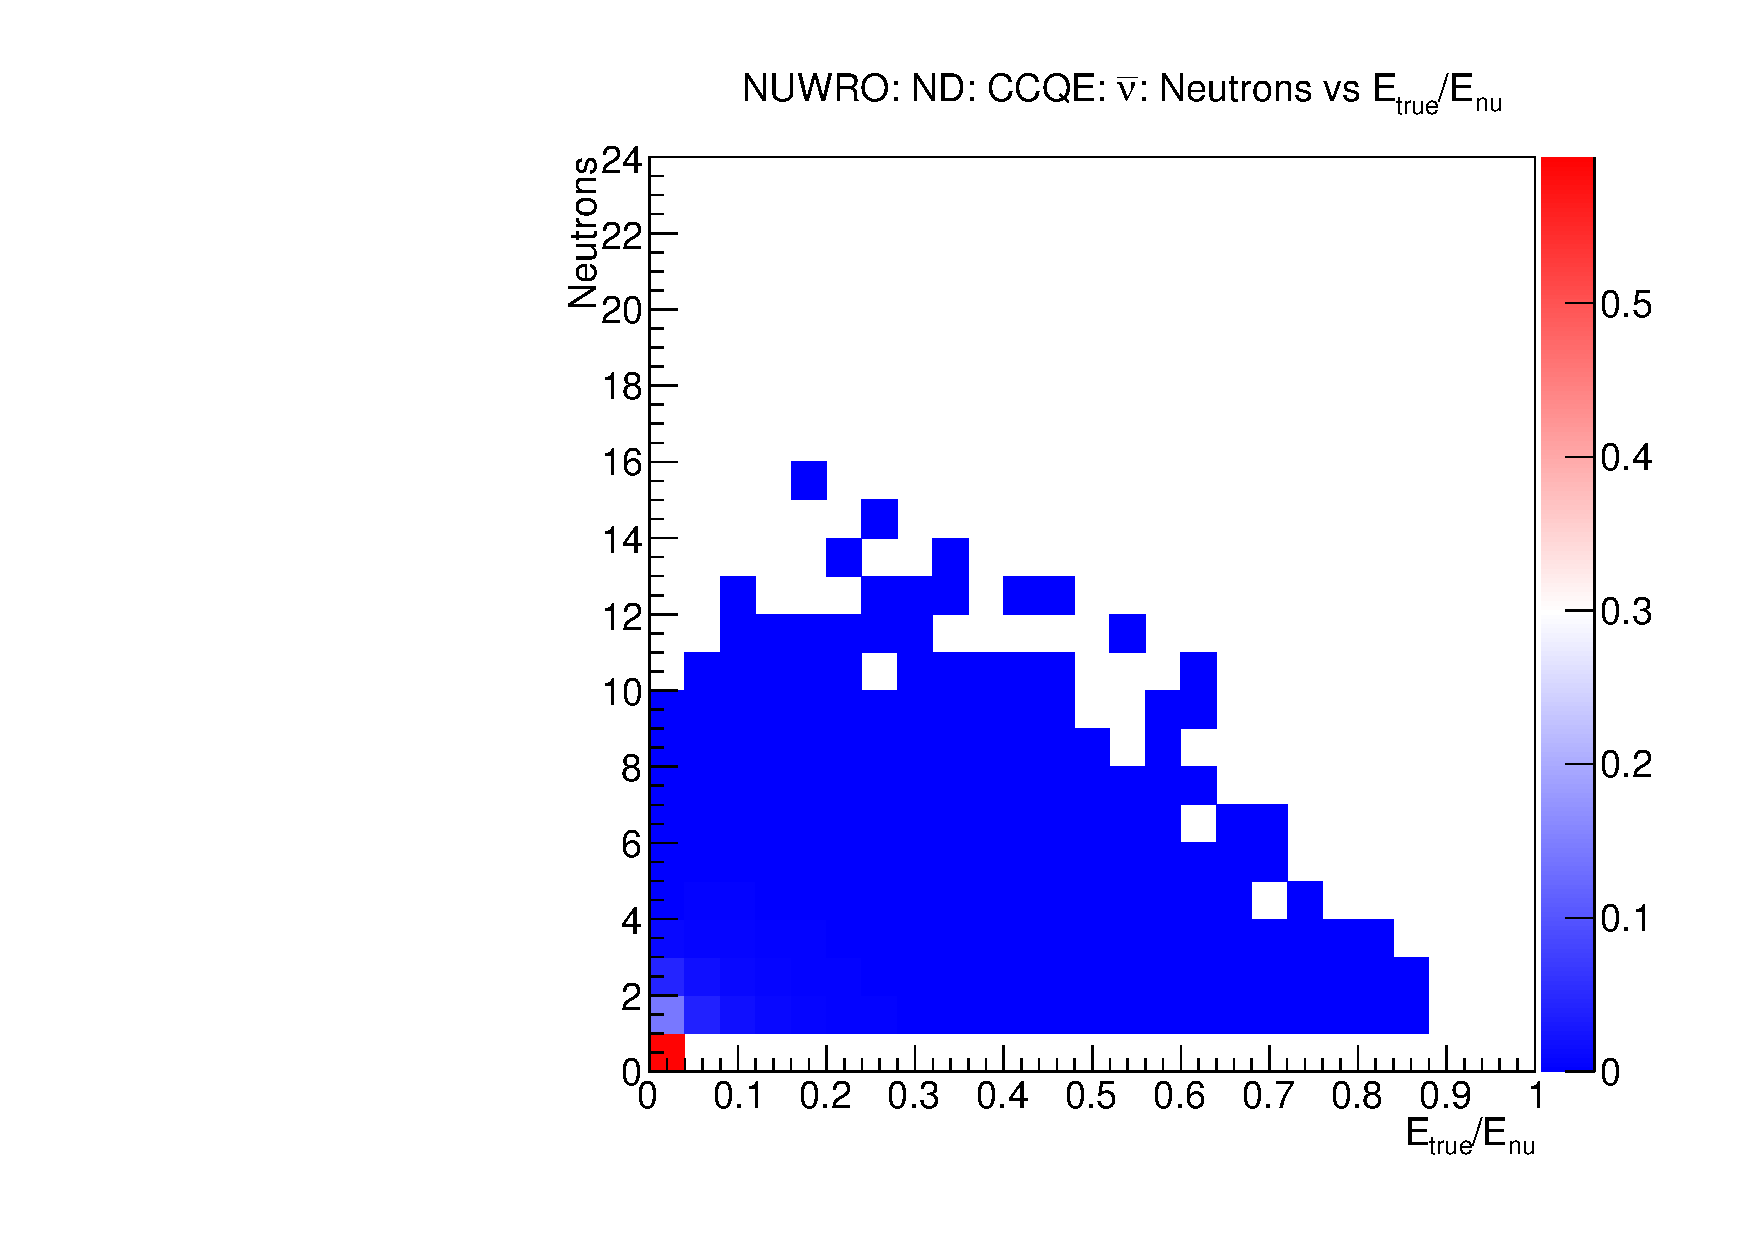
\includegraphics[width=\textwidth]{nneutrons_ene_enu/Nneutrons_Enu_true_ccqe_NUWRO_ND_numub_norm.pdf}
\end{subfigure}
\end{figure}
\FloatBarrier

\subsubsection{2P2H}

These are the same as shown in Section~\ref{subsec:N_multiplicities_Energy}. 

\begin{figure}[!htb]
\centering
\begin{subfigure}[b]{0.32\textwidth}
  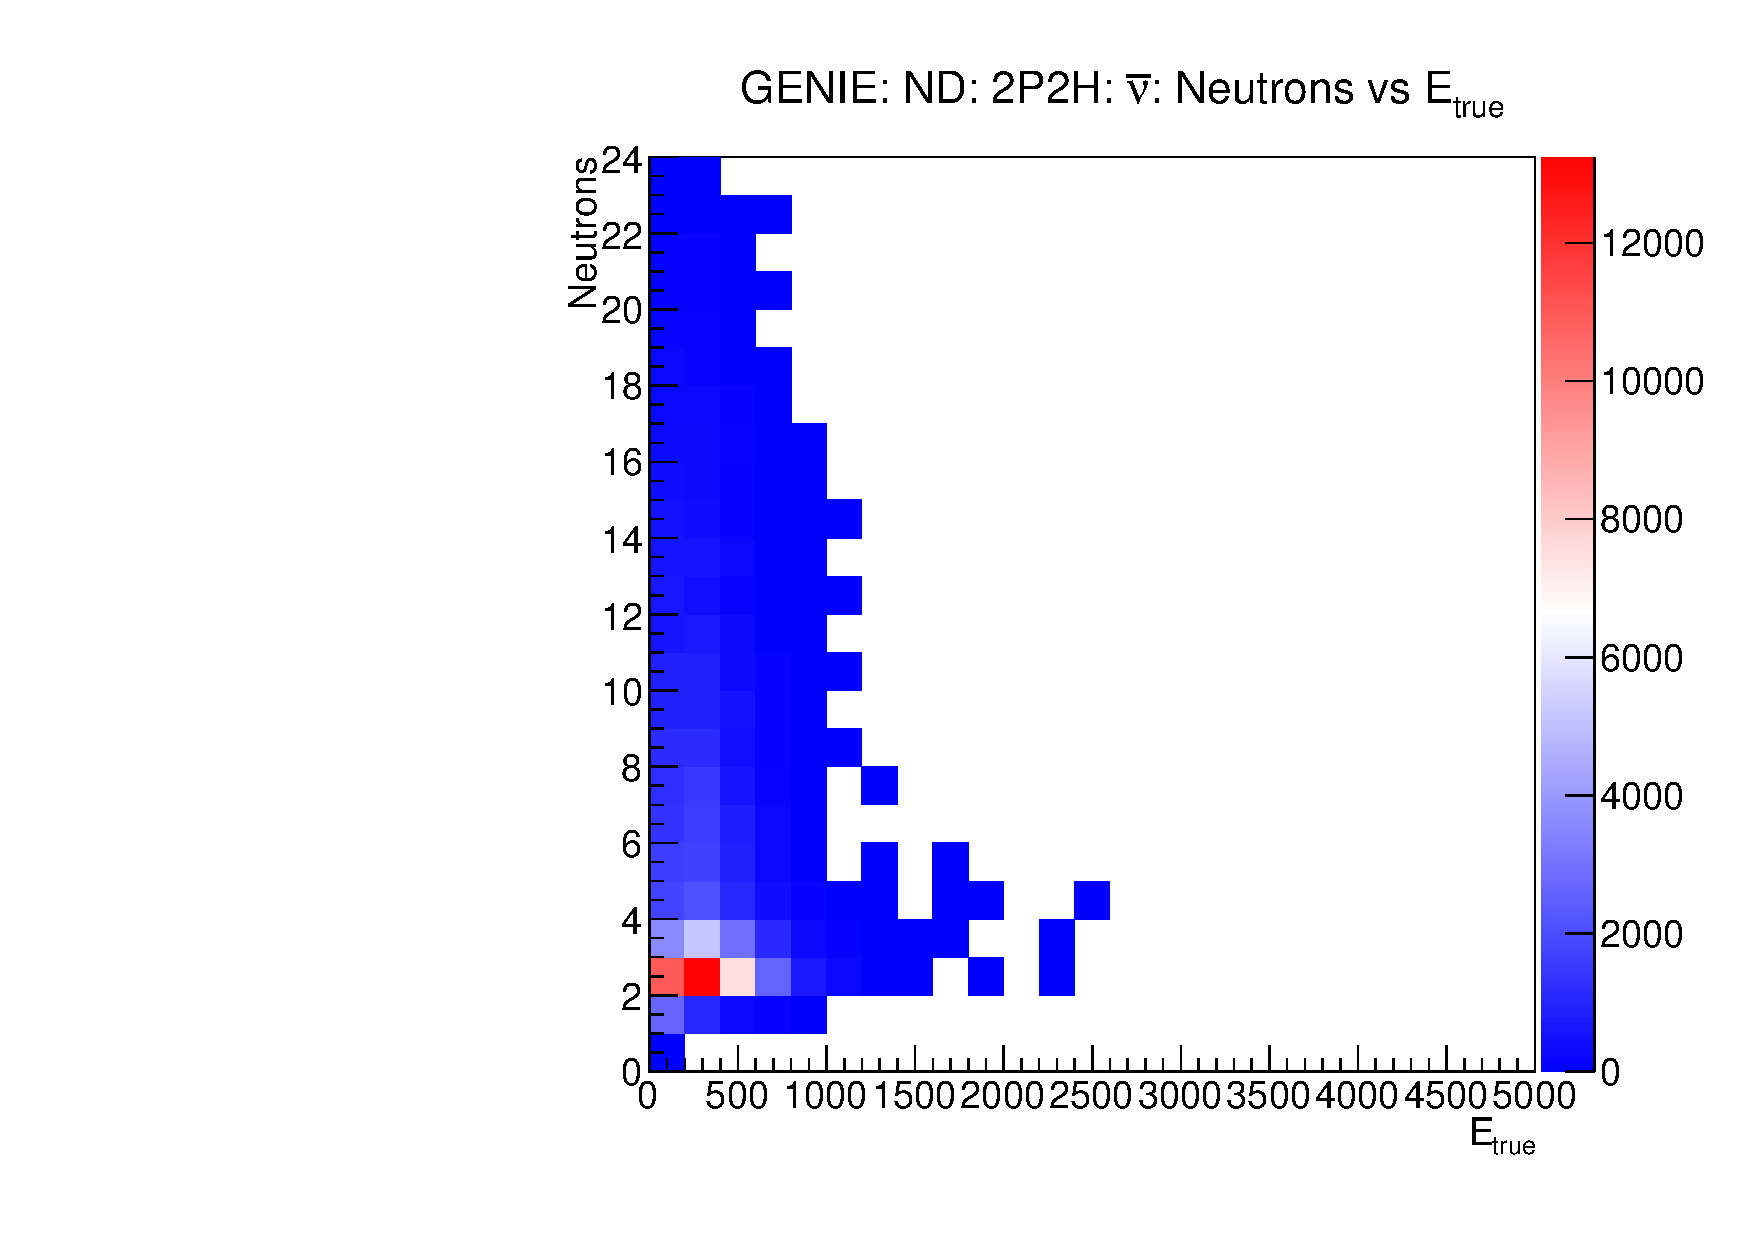
\includegraphics[width=\textwidth]{nneutrons_v_total_ene/Nneutrons_Total_ENe_2p2h_GENIE_ND_numub.pdf}
\end{subfigure}
\begin{subfigure}[b]{0.32\textwidth}
  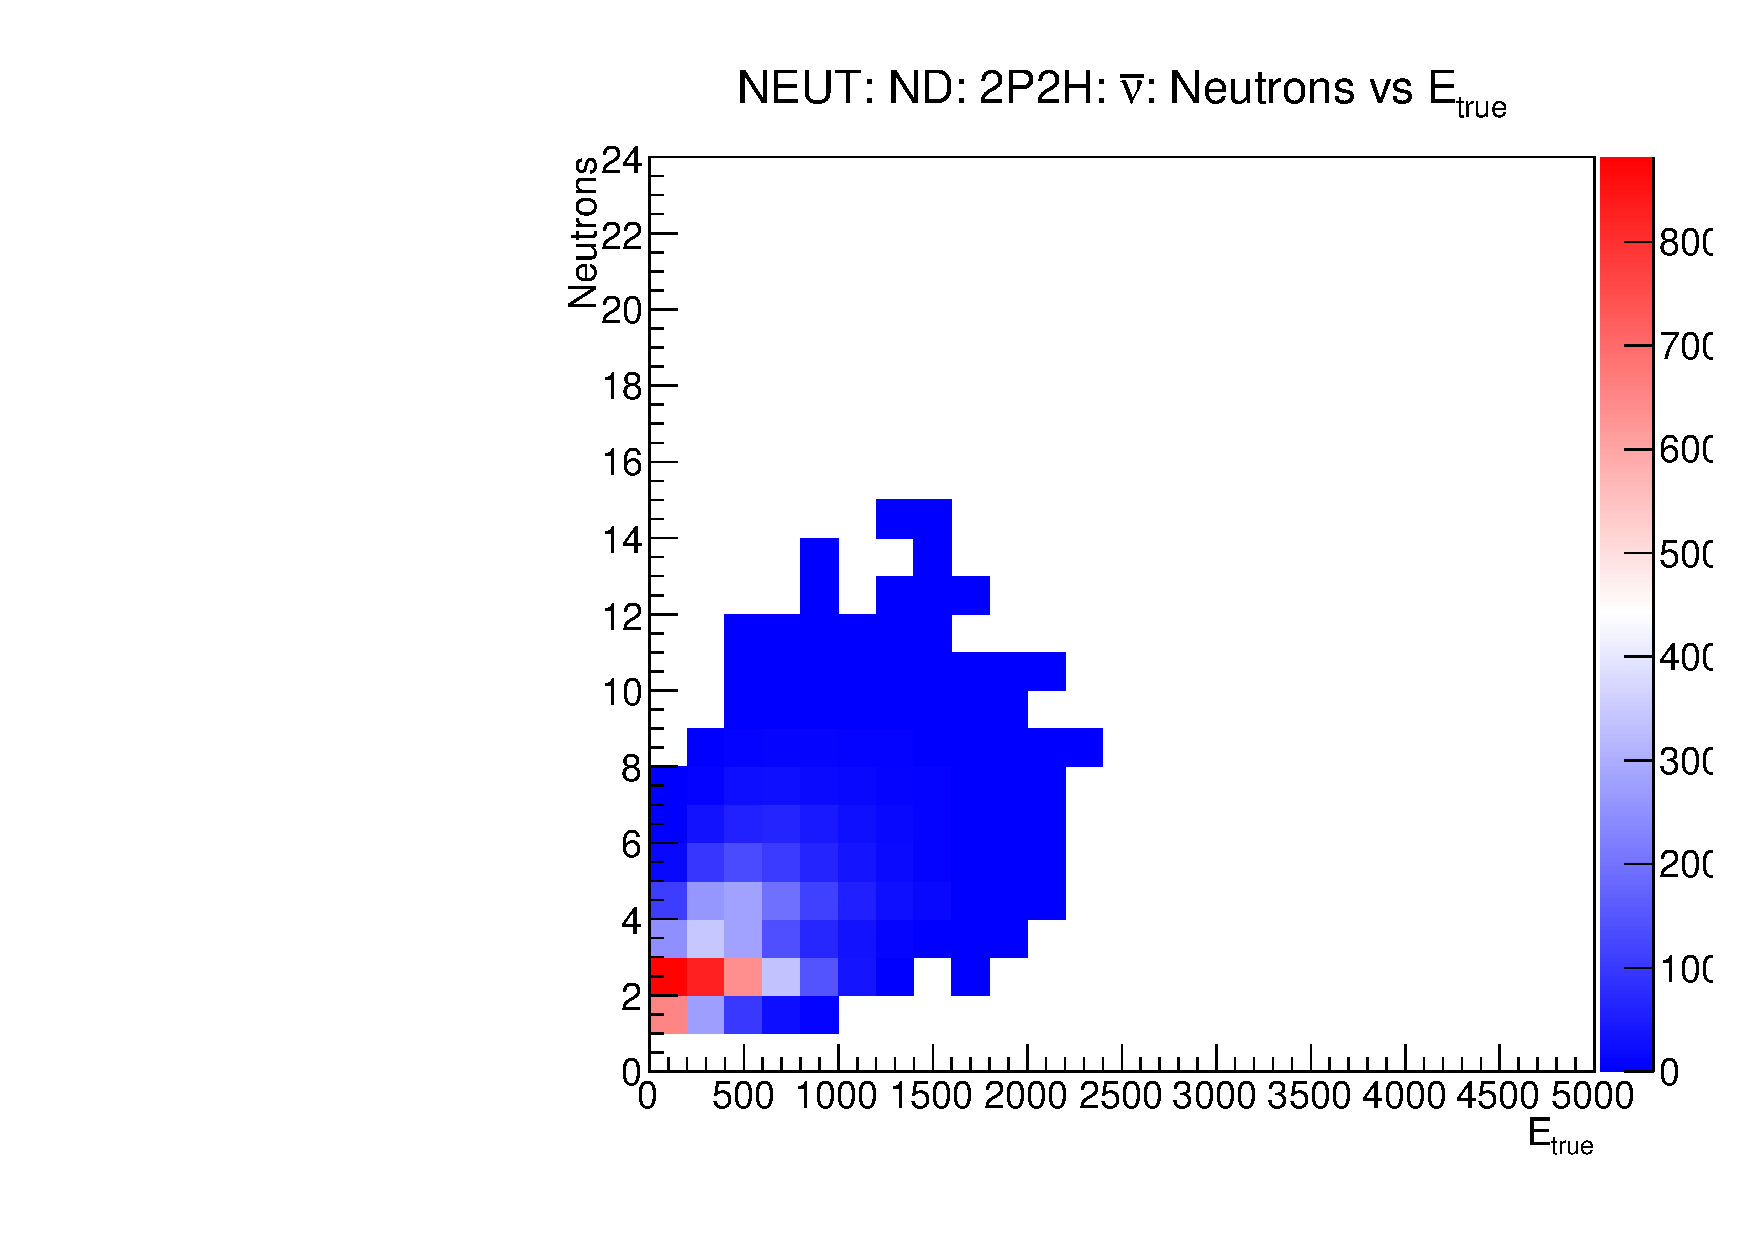
\includegraphics[width=\textwidth]{nneutrons_v_total_ene/Nneutrons_Total_ENe_2p2h_NEUT_ND_numub.pdf}
\end{subfigure}
\begin{subfigure}[b]{0.32\textwidth}
  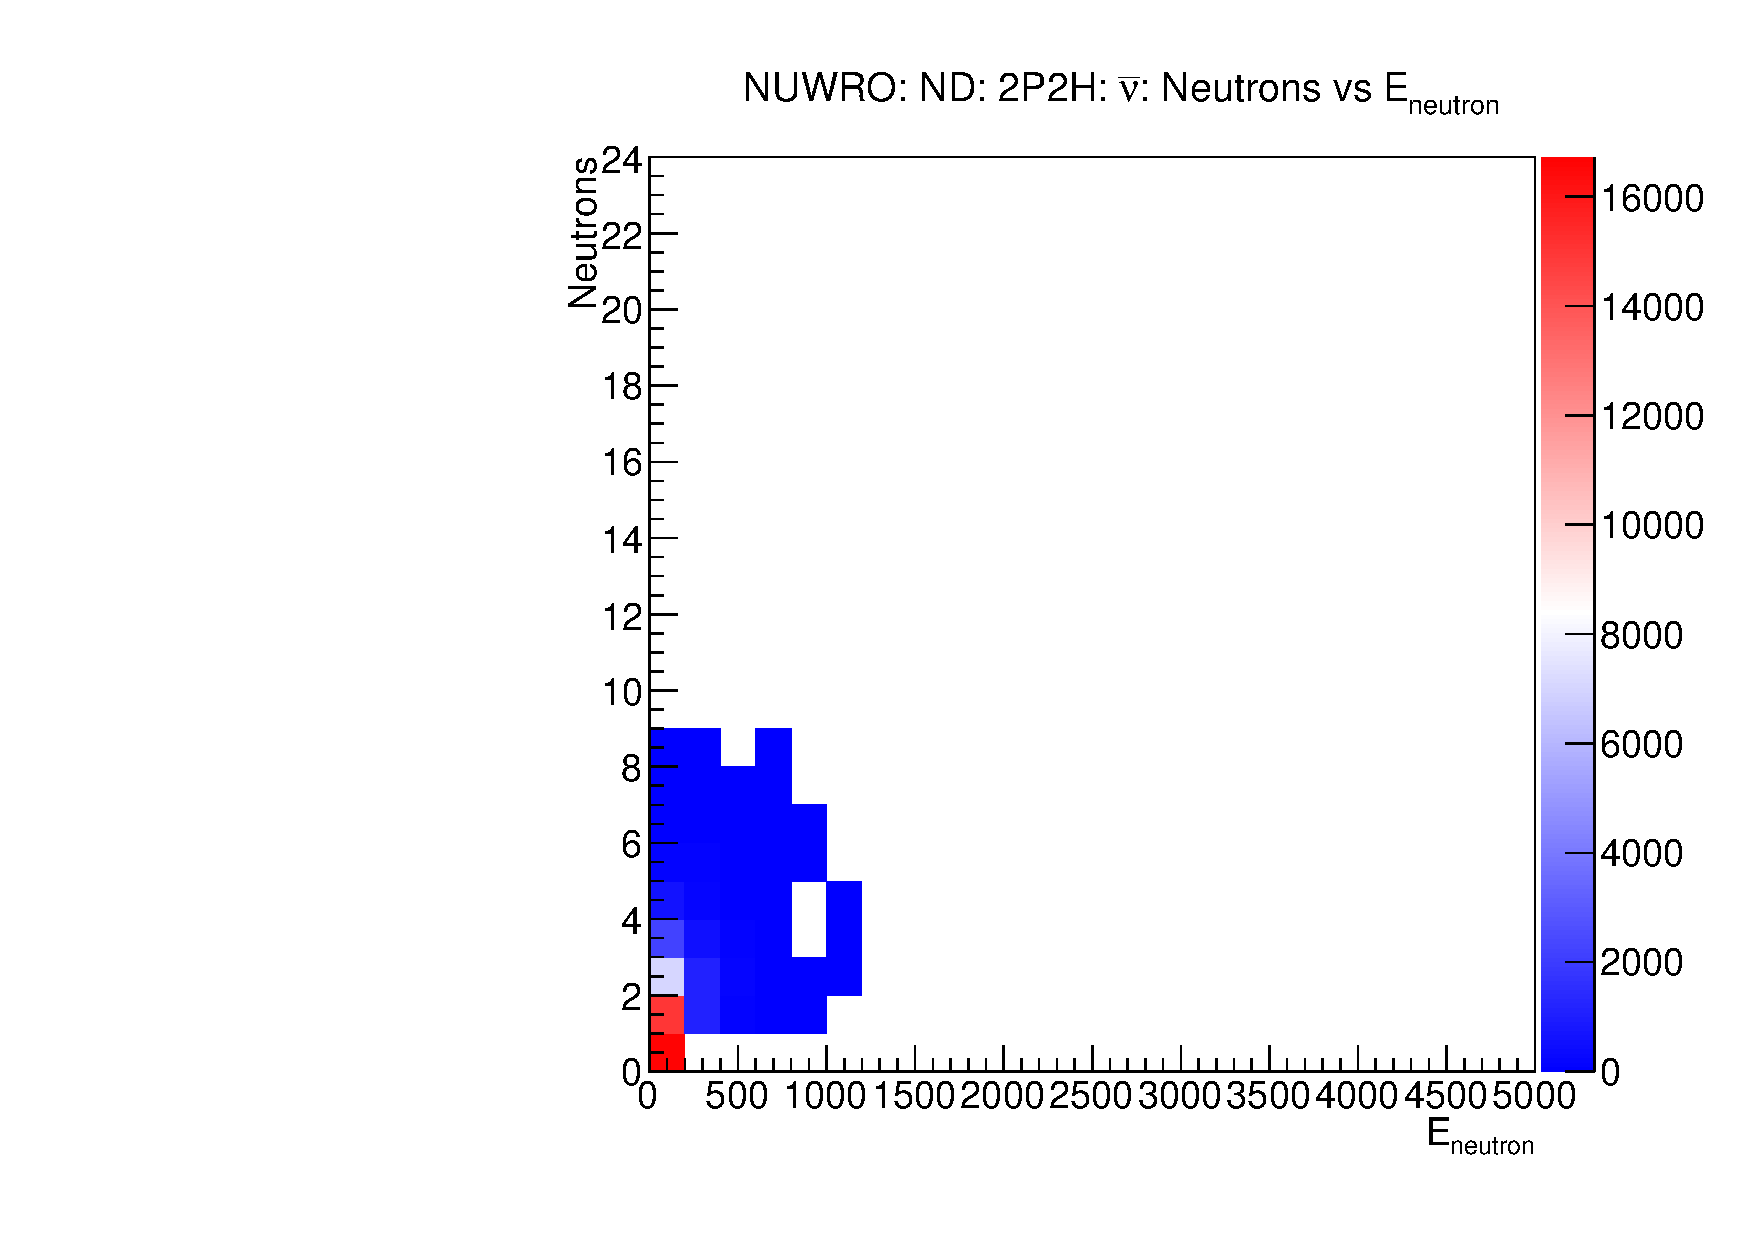
\includegraphics[width=\textwidth]{nneutrons_v_total_ene/Nneutrons_Total_ENe_2p2h_NUWRO_ND_numub.pdf}
\end{subfigure}
\end{figure}

\begin{figure}[!htb]
\centering
\begin{subfigure}[b]{0.32\textwidth}
  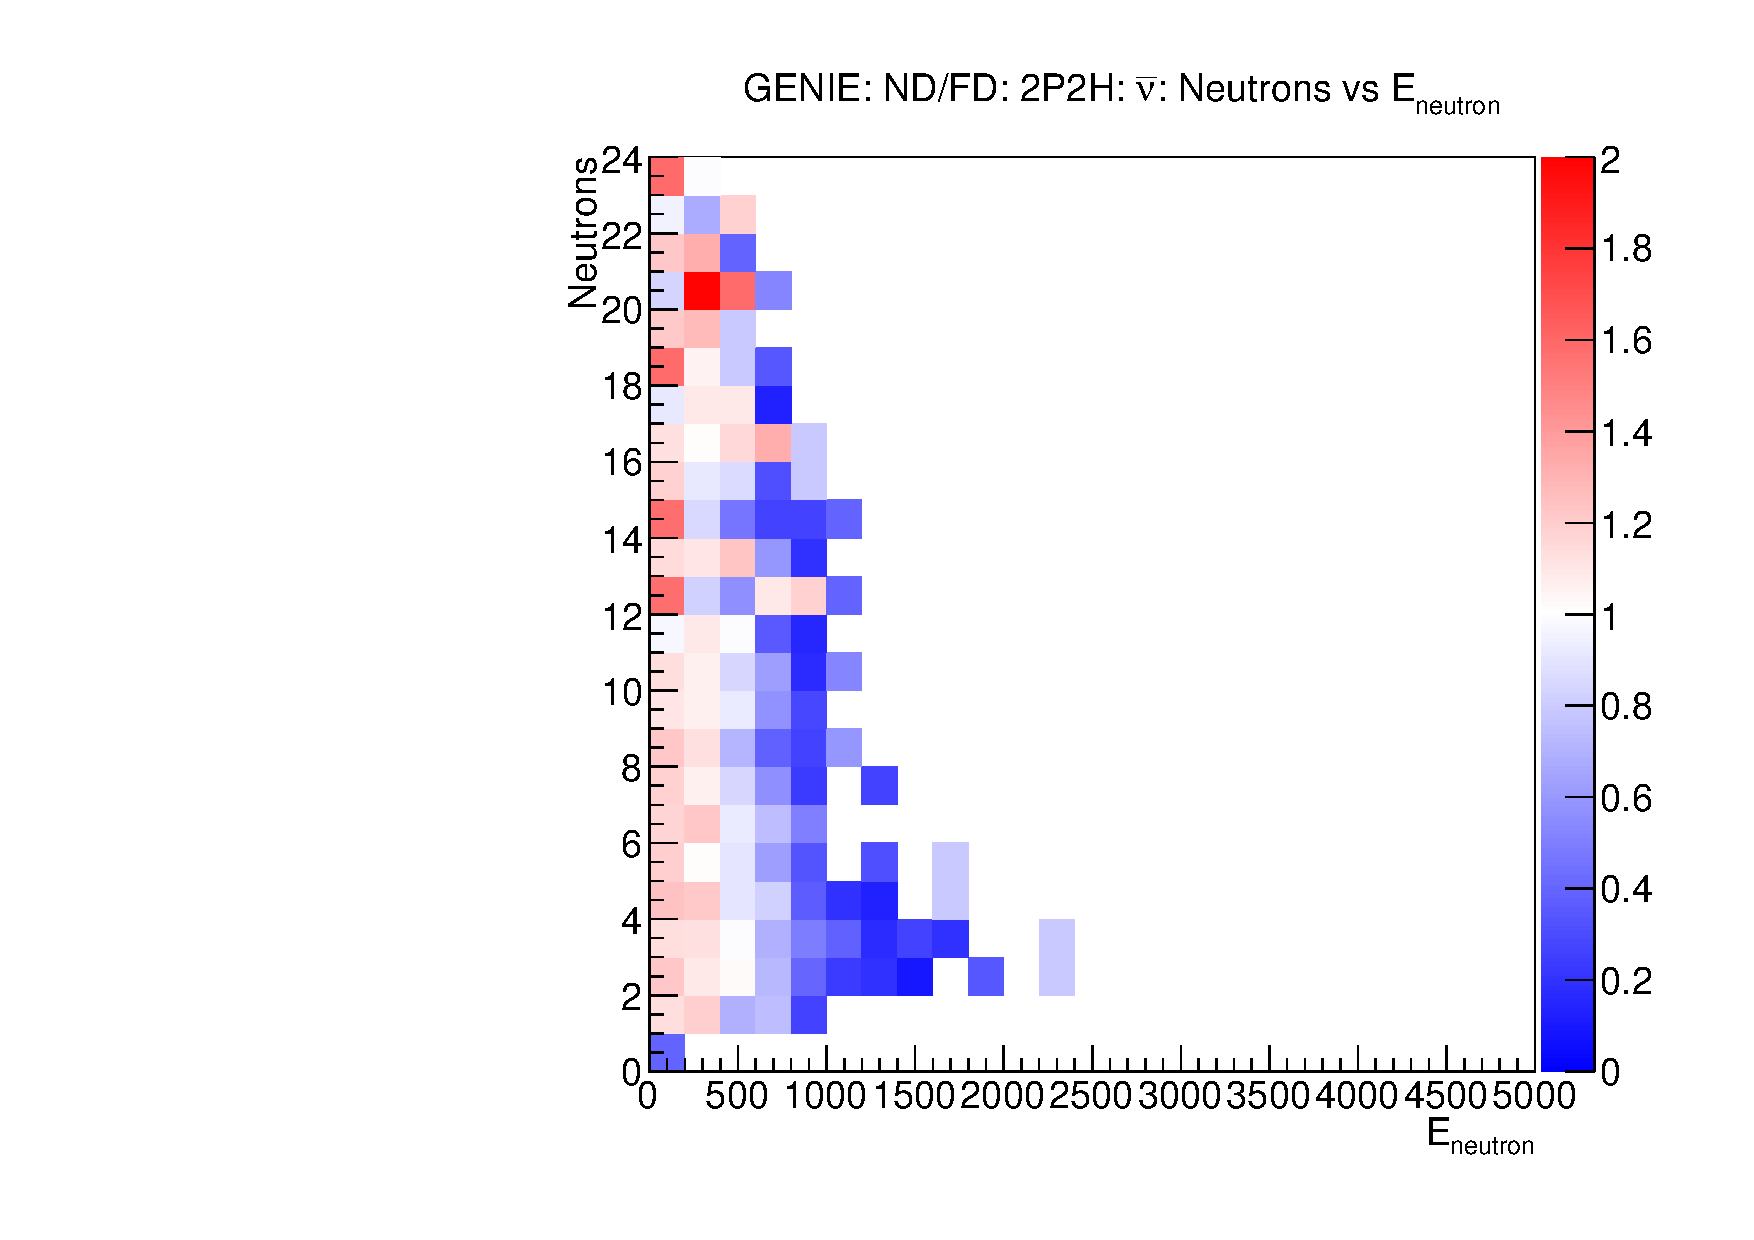
\includegraphics[width=\textwidth]{nneutrons_v_total_ene/Nneutrons_Total_ENe_2p2h_GENIE_ND_FD_numub_norm.pdf}
\end{subfigure}
\begin{subfigure}[b]{0.32\textwidth}
  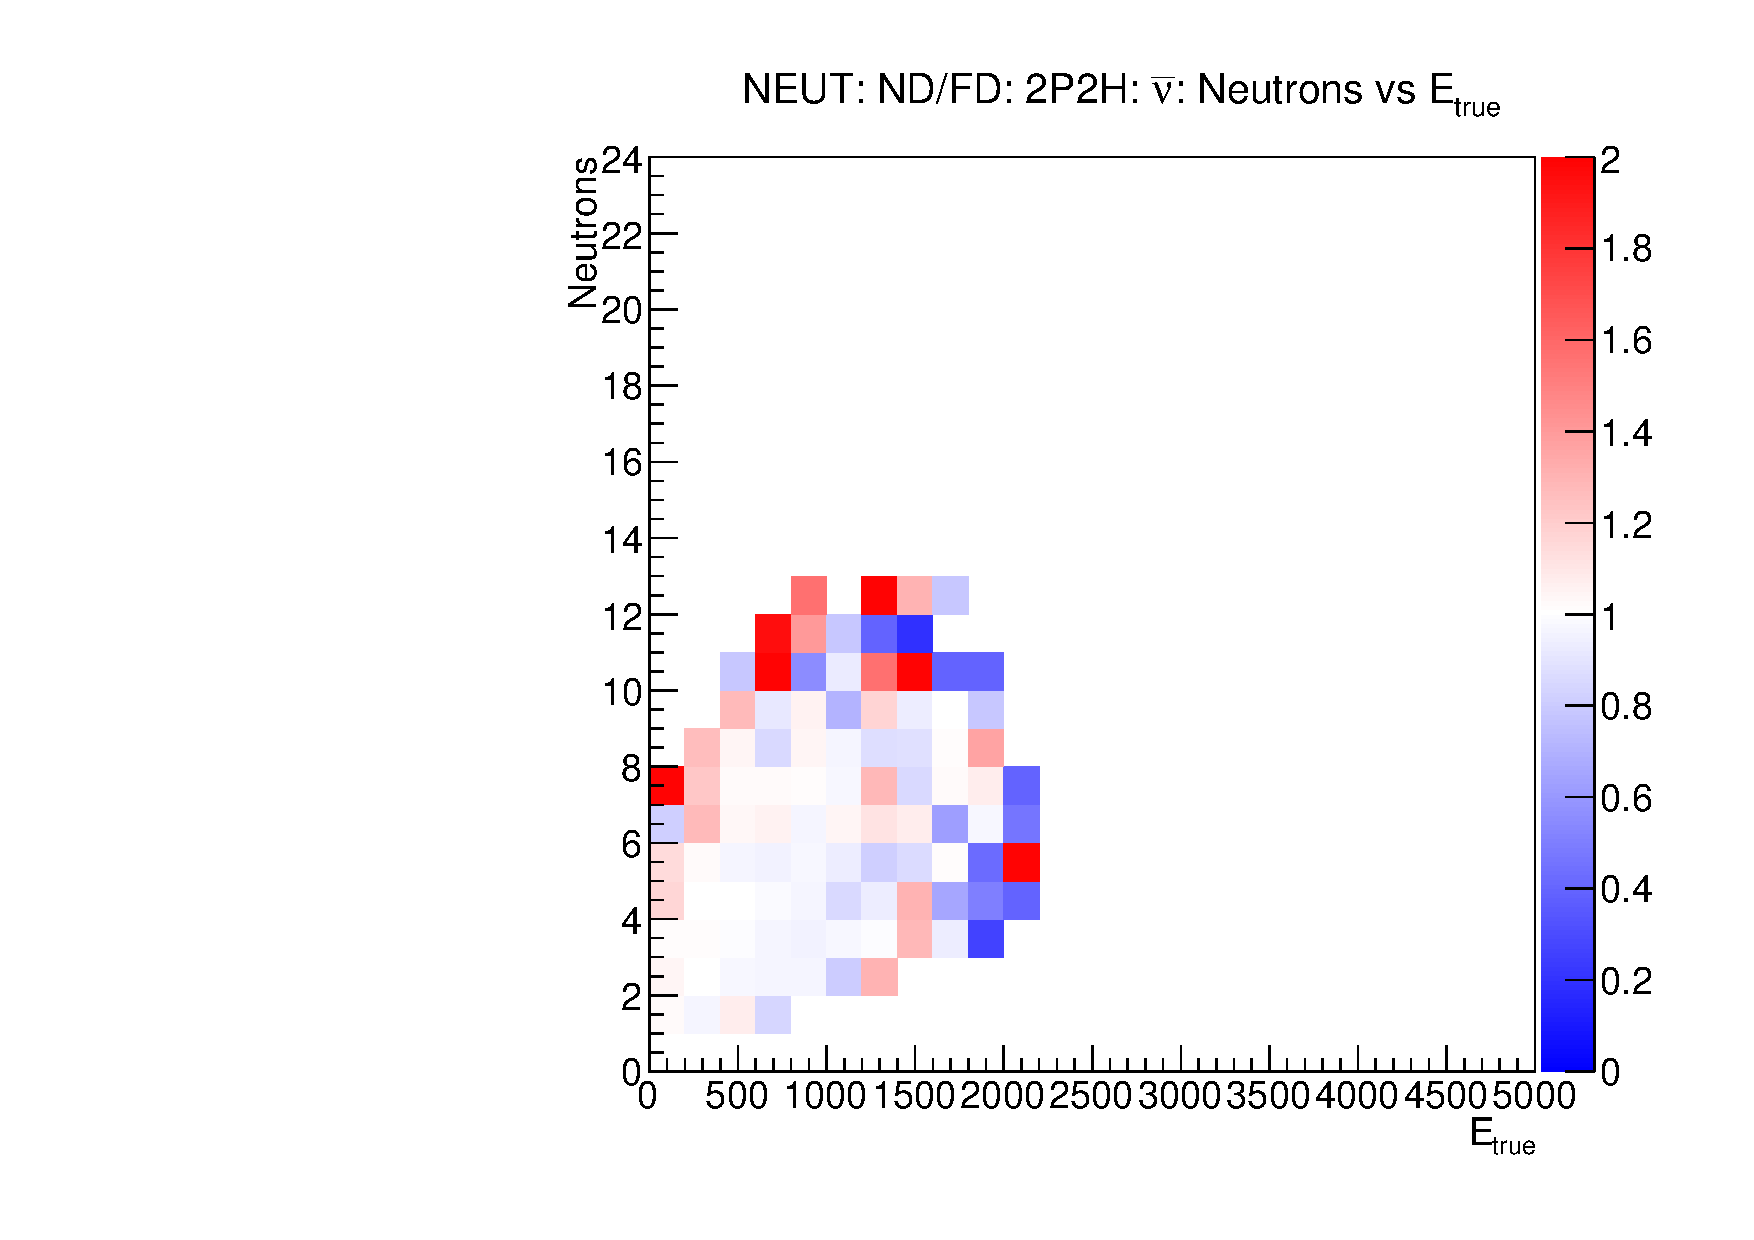
\includegraphics[width=\textwidth]{nneutrons_v_total_ene/Nneutrons_Total_ENe_2p2h_NEUT_ND_FD_numub_norm.pdf}
\end{subfigure}
\begin{subfigure}[b]{0.32\textwidth}
  \includegraphics[width=\textwidth]{nneutrons_v_total_ene/Nneutrons_Total_ENe_2p2h_NUWRO_ND_FD_numub_norm.pdf}
\end{subfigure}
\end{figure}

\begin{figure}[!htb]
\centering
\begin{subfigure}[b]{0.32\textwidth}
  \includegraphics[width=\textwidth]{nneutrons_ene_enu/Nneutrons_Enu_true_2p2h_GENIE_ND_numub_norm.pdf}
\end{subfigure}
\begin{subfigure}[b]{0.32\textwidth}
  \includegraphics[width=\textwidth]{nneutrons_ene_enu/Nneutrons_Enu_true_2p2h_NEUT_ND_numub_norm.pdf}
\end{subfigure}
\begin{subfigure}[b]{0.32\textwidth}
  \includegraphics[width=\textwidth]{nneutrons_ene_enu/Nneutrons_Enu_true_2p2h_NUWRO_ND_numub_norm.pdf}
\end{subfigure}
\end{figure}
\FloatBarrier

\subsubsection{CC1$\pi$}

\begin{figure}[!htb]
\centering
\begin{subfigure}[b]{0.32\textwidth}
  \includegraphics[width=\textwidth]{nneutrons_v_total_ene/Nneutrons_Total_ENe_res_GENIE_ND_numub.pdf}
\end{subfigure}
\begin{subfigure}[b]{0.32\textwidth}
  \includegraphics[width=\textwidth]{nneutrons_v_total_ene/Nneutrons_Total_ENe_res_NEUT_ND_numub.pdf}
\end{subfigure}
\begin{subfigure}[b]{0.32\textwidth}
  \includegraphics[width=\textwidth]{nneutrons_v_total_ene/Nneutrons_Total_ENe_res_NUWRO_ND_numub.pdf}
\end{subfigure}
\end{figure}

\begin{figure}[!htb]
\centering
\begin{subfigure}[b]{0.32\textwidth}
  \includegraphics[width=\textwidth]{nneutrons_v_total_ene/Nneutrons_Total_ENe_res_GENIE_ND_FD_numub_norm.pdf}
\end{subfigure}
\begin{subfigure}[b]{0.32\textwidth}
  \includegraphics[width=\textwidth]{nneutrons_v_total_ene/Nneutrons_Total_ENe_res_NEUT_ND_FD_numub_norm.pdf}
\end{subfigure}
\begin{subfigure}[b]{0.32\textwidth}
  \includegraphics[width=\textwidth]{nneutrons_v_total_ene/Nneutrons_Total_ENe_res_NUWRO_ND_FD_numub_norm.pdf}
\end{subfigure}
\end{figure}

\begin{figure}[!htb]
\centering
\begin{subfigure}[b]{0.32\textwidth}
  \includegraphics[width=\textwidth]{nneutrons_ene_enu/Nneutrons_Enu_true_res_GENIE_ND_numub_norm.pdf}
\end{subfigure}
\begin{subfigure}[b]{0.32\textwidth}
  \includegraphics[width=\textwidth]{nneutrons_ene_enu/Nneutrons_Enu_true_res_NEUT_ND_numub_norm.pdf}
\end{subfigure}
\begin{subfigure}[b]{0.32\textwidth}
  \includegraphics[width=\textwidth]{nneutrons_ene_enu/Nneutrons_Enu_true_res_NUWRO_ND_numub_norm.pdf}
\end{subfigure}
\end{figure}
\FloatBarrier

\subsubsection{CC-Other}

\begin{figure}[!htb]
\centering
\begin{subfigure}[b]{0.32\textwidth}
  \includegraphics[width=\textwidth]{nneutrons_v_total_ene/Nneutrons_Total_ENe_dis_GENIE_ND_numub.pdf}
\end{subfigure}
\begin{subfigure}[b]{0.32\textwidth}
  \includegraphics[width=\textwidth]{nneutrons_v_total_ene/Nneutrons_Total_ENe_dis_NEUT_ND_numub.pdf}
\end{subfigure}
\begin{subfigure}[b]{0.32\textwidth}
  \includegraphics[width=\textwidth]{nneutrons_v_total_ene/Nneutrons_Total_ENe_dis_NUWRO_ND_numub.pdf}
\end{subfigure}
\end{figure}

\begin{figure}[!htb]
\centering
\begin{subfigure}[b]{0.32\textwidth}
  \includegraphics[width=\textwidth]{nneutrons_v_total_ene/Nneutrons_Total_ENe_dis_GENIE_ND_FD_numub_norm.pdf}
\end{subfigure}
\begin{subfigure}[b]{0.32\textwidth}
  \includegraphics[width=\textwidth]{nneutrons_v_total_ene/Nneutrons_Total_ENe_dis_NEUT_ND_FD_numub_norm.pdf}
\end{subfigure}
\begin{subfigure}[b]{0.32\textwidth}
  \includegraphics[width=\textwidth]{nneutrons_v_total_ene/Nneutrons_Total_ENe_dis_NUWRO_ND_FD_numub_norm.pdf}
\end{subfigure}
\end{figure}

\begin{figure}[!htb]
\centering
\begin{subfigure}[b]{0.32\textwidth}
  \includegraphics[width=\textwidth]{nneutrons_ene_enu/Nneutrons_Enu_true_dis_GENIE_ND_numub_norm.pdf}
\end{subfigure}
\begin{subfigure}[b]{0.32\textwidth}
  \includegraphics[width=\textwidth]{nneutrons_ene_enu/Nneutrons_Enu_true_dis_NEUT_ND_numub_norm.pdf}
\end{subfigure}
\begin{subfigure}[b]{0.32\textwidth}
  \includegraphics[width=\textwidth]{nneutrons_ene_enu/Nneutrons_Enu_true_dis_NUWRO_ND_numub_norm.pdf}
\end{subfigure}
\end{figure}
\FloatBarrier


